%%%%%%%%%%%%%%%%%%%%  bare_jrnl.tex V1.2 2002/11/18  %%%%%%%%%%%%%%%%%%%%%%%

%% This is a skeleton file demonstrating the use of IEEEtran.cls
%% (requires IEEEtran.cls version 1.6b or later) with an IEEE journal paper.

%\documentclass[10pt]{IEEEtran}
\documentclass[11pt,draftcls,onecolumn]{IEEEtran}

%%%%%%%%%%%%%%%%%%%  PACKAGES AND DEFINITIONS%%%%%%%%%%%%%%%%%

\usepackage{epsfig}
\usepackage{amsmath}
\usepackage{multirow}
\usepackage{amsmath,graphicx}
\usepackage{pgf}
\usepackage{tikz}
\usepackage{subfig}
\usetikzlibrary{backgrounds,shapes,snakes}
\usetikzlibrary{calc,chains,positioning}
\usepackage{phaistos}
\usepackage{cases}
\usepackage{pgfplots}
\usepackage{empheq}
\DeclareMathOperator{\diag}{diag}
%%%%%%%%%%%%%%%%%%%%%%%%%%%%%%%%%%%%%%%%%%%%%%%%%%%%%%%%%%%%%%

% correct bad hyphenation here
%\hyphenation{}

\begin{document}
\newlength\figureheight
\newlength\figurewidth
\setlength\figureheight{3.6cm}
\setlength\figurewidth{6.5cm}
\title{On Least Squares Equalization and Channel Shortening for Speech Dereverberation}

\date{June 24, 2013}

\author{Ina Kodrasi*,~\IEEEmembership{Student Member,~IEEE,} Simon Doclo,~\IEEEmembership{Senior Member,~IEEE}% <-this % stops a space
\thanks{The authors are with the Signal Processing Group, Department of Medical Physics and Acoustics, and Cluster of Excellence Hearing4All, University of Oldenburg, Oldenburg, Germany (e-mail: \mbox{ina.kodrasi@uni-oldenburg.de}; simon.doclo@uni-oldenburg.de).}
\thanks{
This work was supported in part by a Grant from the GIF, the German-Israeli Foundation for Scientific Research and Development, the Cluster of Excellence 1077 ``Hearing4All'' funded by the German Research Foundation (DFG), and the Marie Curie Initial Training Network DREAMS (Grant no. 316969).}
}

\markboth{IEEE Signal Processing Letters}{Kodrasi and Doclo: On Least Squares Equalization and Channel Shortening for Speech Dereverberation}


\maketitle

\begin{abstract}

In this letter, a generalized framework for least squares acoustic multichannel equalization techniques is established, which enables to analyze the properties~(i.e., existence and uniqueness) of the resulting reshaping filters.
It is shown that least squares equalization techniques yield reshaping filters that lie in the subspace spanned by the multiple solutions maximizing the so-called channel shortening~(CS) cost function.
Since least squares reshaping filters have been experimentally validated to yield a trade-off between reverberant tail suppression and perceptual speech quality preservation and they lie in the subspace of CS solutions, it can be said that the multiple CS solutions offer the potential to achieve a high performance both in terms of reverberant tail suppression and perceptual speech quality preservation.
Hence, a novel subspace-based equalization~(SuB) technique is proposed, which constrains the reshaping filter to be a linear combination of the multiple CS solutions. 
Simulation results illustrate the high dereverberation performance of the proposed technique.
\end{abstract}

\begin{keywords}
least squares equalization, channel shortening, subspace-based equalization
\end{keywords}

%==============================================================================================================
\section{Introduction}
Acoustic multichannel equalization comprises an attractive approach to speech dereverberation due to its potential to theoretically achieve perfect dereverberation~\cite{Miyoshi_ITASS_1988,Kodrasi_ITASLP_2013}.
However, in practice such an approach remains challenging given its sensitivity to estimation errors in the room impulse responses~(RIRs) between the source and the microphone array~\cite{Kodrasi_ITASLP_2013,Zhang_IWAENC_2010}.
Over the past decades, several acoustic multichannel equalization techniques have been proposed~\cite{Miyoshi_ITASS_1988,Kodrasi_ITASLP_2013,Zhang_IWAENC_2010,Lim_IWAENC_2012,Kallinger_ICASSP_2006,Lim_ICASSP_2013,Lim_WASPAA_2013,Mertins_ITASLP_2010,Jungmann_ICASSP_2014}.
On the one hand, least squares equalization techniques such as the multiple-input/output inverse theorem~(MINT)-based technique~\cite{Miyoshi_ITASS_1988}, the partial multichannel equalization technique based on MINT~(P-MINT)~\cite{Kodrasi_ITASLP_2013}, the relaxed multichannel least squares technique~(RMCLS)~\cite{Zhang_IWAENC_2010}, and the relaxed multichannel least squares technique with constrained initial taps~(RMCLS-CIT)~\cite{Lim_IWAENC_2012}, design reshaping filters such that the (weighted) system response equals a given (weighted) target response. 
On the other hand, channel shortening aims at an overall system response with maximum energy in the direct path and early reflections and minimum energy in the reverberant tail.
In~\cite{Zhang_IWAENC_2010} it has been shown that multiple solutions exist which maximize the CS cost function.
Furthermore, in~\cite{Kodrasi_ITASLP_2013} and~\cite{Zhang_IWAENC_2010} it has been proven that the reshaping filters designed using the MINT and P-MINT techniques can be expressed as linear combinations of these multiple CS solutions.

The aim of this letter is twofold.
Firstly, a generalized framework for state-of-the-art least squares equalization techniques is established. 
A theoretical analysis based on the Rouch\'{e}-Capelli theorem~\cite{shafarevic_algebra_book} is provided to determine the properties~(i.e., existence and uniqueness) of the solution(s) for each technique.
Using this analysis, it can be shown that state-of-the-art least squares equalization techniques yield reshaping filters which lie in the subspace spanned by the multiple CS solutions.
Although this result may appear trivial, to the best of our knowledge it was not yet available in the literature.
Secondly, the subspace of CS solutions is exploited to derive a novel subspace-based equalization~(SuB) technique aiming at achieving a high reverberant tail suppression and perceptual speech quality preservation. 
Experimental results demonstrate the advantage of the proposed technique as compared to the least squares equalization techniques in the presence of RIR estimation errors.
%==============================================================================================================

\section{Acoustic Multichannel Equalization}
\subsection{Problem Formulation}
Consider an acoustic system with a single speech source and $M$ microphones as depicted in Fig.~\ref{fig: acsys}.
The $m$-th microphone signal $x_m(n)$ at time index $n$ is given by 
\begin{equation}
x_m(n) = s(n) \ast h_m(n), \; \; \; \; \; m = 1, \; \ldots, \; M,
\end{equation}
with $s(n)$ the clean speech signal, $h_m(n)$ the $L_h$ taps long RIR between the source and the $m$-th microphone, i.e., $\mathbf{h}_m = \left[h_m(0) \; h_m(1) \; \ldots \; h_m(L_h-1) \right]^T$, and $\ast$ denoting convolution.
Equalization techniques apply filters $\mathbf{g}_m$ of length $L_g$, i.e., $\mathbf{g}_m = \left[g_m(0) \; g_m(1) \; \ldots \; g_m(L_g-1) \right]^T$, such that the output of the system $\hat{s}(n)$ is given by
\begin{equation}
  \hat{s}(n) = \sum_{m=1}^{M} x_m(n) \ast g_m(n) = s(n) \ast \underbrace{\sum_{m=1}^{M} h_m(n) \ast g_m(n)}_{c(n)},
\end{equation}
\begin{figure}[t!]
  \centering
  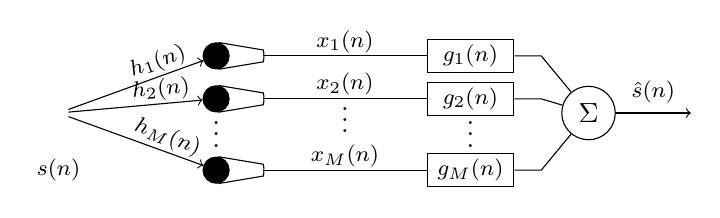
\begin{tikzpicture}
    % Adjustments
    \def\micd{.1cm}                % mic diameter
    \def\micl{.6cm}                % mic length
    \def\micw{.15cm}               % mic width
    \def\micbend{10}               % mic bottom bend
    \def\micdistance{.2cm}         % distance between microphones
    \def\filterdistance{2.5cm}     % distance between microphone and filter
    \def\filteroutline{.9cm}       % length of line which gets out of filter
    \def\sumdistance{1.5cm}        % distance of sum node to the filter
    \def\sumoutline{1cm}           % length of line which gets out of sum
    \def\headdistance{2cm}         % distance between microphone and head

    % Styles
    \tikzset{%
      mic head/.style={fill=black,draw=black,circle,minimum size=\micd},
      filter/.style={draw,minimum width=1.1cm,inner sep=2pt},
      sum/.style={draw,circle},
      xlabel/.style={inner sep=1pt,above,midway},
      sumlabel/.style={xlabel},
      hlabel/.style={xlabel,sloped,pos=.7},
      head/.style={font=\Large}
    }

    % Draw Microphones
    \begin{scope}[start chain=going below,every node/.style={on chain},node distance=\micdistance]
      \node[mic head] (mic1) {};
      \node[mic head] (mic2) {};
      \node[mic head,yshift=-1.8*\micdistance] (mic3) {};
    \end{scope}
    \node[yshift=3pt] at ($(mic2)!.5!(mic3)$) {$\vdots$};

    \foreach \m in {1,2,3} {%
      \coordinate (m1) at ($(mic\m)+(\micl,\micw/2)$);
      \coordinate (m2) at ($(mic\m)+(\micl,-\micw/2)$);
      \draw (tangent cs:node=mic\m,point={(m1)},solution=1) -- (m1) to[bend left=\micbend] (m2) -- (tangent cs:node=mic\m,point={(m2)},solution=2);
    }

    % Draw Filter
    \foreach \m/\i in {1/1,2/2,3/M} {%
      \node[filter,right=\filterdistance of mic\m] (filter\m) {\footnotesize $g_{\i}(n)$};
      \draw ($(mic\m)+(\micl,0)$) to node[xlabel] (x\m) {\footnotesize $x_{\i}(n)$} (filter\m);
    }
    \node[yshift=3pt] at ($(filter2)!.5!(filter3)$) {$\vdots$};
    \node[yshift=3pt] at ($(x2)!.5!(x3)$) {$\vdots$};
    % Sum Node
    \node[sum] (sum) at ($(filter1)!.5!(filter3)+(\sumdistance,0)$) {$\Sigma$};
    \draw[->] (sum) -- node[above] {\footnotesize $\hat{s}(n)$} ++(1.3,0);
    % Connect filter with sum
    \foreach \m in {1,2,3} {%
      \draw (filter\m) -- ++(\filteroutline,0) -- (sum);
    }

    % Head
    \node[head] (head) at ($(mic1)!.5!(mic3)-(\headdistance,0)$) {\PHtattooedHead};
    \node[fill=white,minimum width=4.8pt,minimum height=5.7pt,inner sep=0pt] at ($(head.center)+(2.3pt,-2.5pt)$) {};
    \node at ($(head.center)+(0.0pt,-20.5pt)$) {\footnotesize $s(n)$};
    % Connect head with mics
    \foreach \m/\i in {1/1,2/2,3/M} {%
      \draw[->] (head) -- node[hlabel] {\footnotesize $h_{\i}(n)$} (mic\m);
    }
  \end{tikzpicture}
  \caption{Multichannel equalization system.}
  \label{fig: acsys}
\end{figure}
with $c(n)$ denoting the overall response between the source and the output, referred to as the equalized impulse response~(EIR).
The EIR of length $L_c = L_h+L_g-1$ can be described in vector notation as $\mathbf{c} = \left[c(0) \; c(1) \; \ldots \; c(L_c-1) \right]^{T}$.
Using the $ML_g$--dimensional reshaping filter 
\begin{equation}
\mathbf{g}  =  \left[\mathbf{g}_1^T \; \mathbf{g}_2^T \; \ldots \; \mathbf{g}_M^T \right]^T
\end{equation}
and the $L_c \times ML_g$--dimensional multichannel convolution matrix $\mathbf{H}$, i.e.,
\begin{equation}
\mathbf{H} = \left[\mathbf{H}_1 \; \mathbf{H}_2 \; \ldots \; \mathbf{H}_M \right],
\end{equation}
with $\mathbf{H}_m$ the convolution matrix of $h_m(n)$, the EIR can be expressed as $\mathbf{c} = \mathbf{H}\mathbf{g}$.
The reshaping filter can then be constructed based on different design objectives for the EIR $\mathbf{c}$.
Since the true RIRs are typically not available in practice~\cite{Radlovic_ITSA_2000,Hasan_EUSIPCO_2006,Lin_ITASLP_2012}, equalization techniques design $\mathbf{g}$ using the estimated multichannel convolution matrix $\hat{\mathbf{H}}$~(constructed from the estimated RIRs $\hat{h}_m(n)$), hence optimizing the estimated EIR
\begin{equation}
\boxed{\hat{\mathbf{c}} = \hat{\mathbf{H}}\mathbf{g}}
\end{equation}
Under the assumptions typically made in acoustic multichannel equalization~\cite{Miyoshi_ITASS_1988}, i.e., 
\begin{itemize}
  \item the estimated RIRs do not share any common zeros, and
  \item $L_g \geq \lceil{\frac{L_h-1}{M-1}\rceil}$,
\end{itemize}
the estimated multichannel convolution matrix $\hat{\mathbf{H}}$ is assumed to be a full row-rank matrix~\cite{Harikumar_ITSP_1998}.

In the following, the optimization criteria of state-of-the-art equalization techniques are reviewed.
\subsection{Least Squares Equalization Techniques}
The aim of least squares equalization is to design a reshaping filter $\mathbf{g}$ such that the~(weighted)~EIR equals a~(weighted)~target EIR $\mathbf{c}_t$. 
Formally, these techniques seek to compute a solution $\mathbf{g}$ to the system of equations
\begin{equation}
  \label{eq: lsg}
\boxed{\mathbf{W}\hat{\mathbf{H}}\mathbf{g} = \mathbf{W}\mathbf{c}_t}
\end{equation}
with $\mathbf{W}$ being a diagonal weighting matrix.
The definition of the weighting matrix $\mathbf{W}$ and target EIR $\mathbf{c}_t$ for MINT~\cite{Miyoshi_ITASS_1988}, P-MINT~\cite{Kodrasi_ITASLP_2013}, RMCLS~\cite{Zhang_IWAENC_2010}, and RMCLS-CIT~\cite{Lim_IWAENC_2012} is presented in Tables~\ref{tbl: wls} and~\ref{tbl: tls} respectively, where $\mathbf{I}$ is the $L_c \times L_c$--dimensional identity matrix, $\tau$ denotes a delay in number of samples, $L_d$ is the length in number of samples of the direct path and early reflections, $L_r$ is the number of taps to constrain in RMCLS-CIT, and $p \in \{1, \; \ldots, \; M \}$.
\begin{table}[b!]
  \centering
  \caption{Definition of the weighting matrix $\mathbf{W}$ for state-of-the-art least squares equalization techniques.}
  \label{tbl: wls}
  \begin{tabular}{|l|r|}
    \hline
    Technique & Weighting matrix $\mathbf{W}$ \\
    \hline
     MINT & $\mathbf{I}$ \\
    \hline
    P-MINT & $\mathbf{I}$ \\
    \hline
    RMCLS & $\mathbf{W}_c = {\diag}[\underbrace{1 \; \ldots \; 1}_{\tau} \; \underbrace{1 \; 0 \; \ldots \; 0}_{L_d} \; 1 \; \ldots 1]^{T}$\\
    \hline
    RMCLS-CIT & $\mathbf{W}_{r} = {\diag} [\underbrace{1 \; \ldots \; 1}_{\tau} \; \underbrace{1 \; 1 \; \ldots \; 1}_{L_{r}} \; \underbrace{0 \; \ldots 0}_{L_d-L_{r}} \; 1 \; \ldots 1]^{T}$\\
    \hline
  \end{tabular}
\end{table}
\begin{table}[b!]
  \centering
  \caption{Definition of the target EIR $\mathbf{c}_t$ for state-of-the-art least squares equalization techniques.}
  \label{tbl: tls}
  \begin{tabular}{|l|r|}
    \hline
    Technique & Target EIR $\mathbf{c}_t$ \\
    \hline
    MINT & $\mathbf{d} = [\underbrace{0 \; \ldots \; 0}_{\tau} \; 1 \; 0 \; \ldots \; 0 ]^T$ \\
    \hline
    P-MINT & $\hat{\mathbf{h}}_{p}^{\rm d} = [\underbrace{0\phantom{\rlap{$(L_d-1)$}} \ldots 0 }_{\tau} \underbrace{\hat{h}_p(0) \ldots \hat{h}_p(L_d-1)}_{L_d} 0 \ldots 0 ]^{T}$  \\
    \hline
    RMCLS & $\mathbf{d} = [\underbrace{0 \; \ldots \; 0}_{\tau} \; 1 \; 0 \; \ldots \; 0 ]^T$ \\
    \hline
    RMCLS-CIT & $\hat{\mathbf{h}}_{p}^{\rm d} = [\underbrace{0\phantom{\rlap{$(L_d-1)$}} \ldots 0 }_{\tau} \underbrace{\hat{h}_p(0) \ldots \hat{h}_p(L_d-1)}_{L_d} 0 \ldots 0 ]^{T}$ \\
    \hline
  \end{tabular}
\end{table}
From these definitions of $\mathbf{W}$ and $\mathbf{c}_t$, it can be observed that on the one hand, techniques such as MINT and P-MINT aim at setting all taps of the resulting EIR to a desired target EIR, which results in a good perceptual speech quality preservation but low reverberant tail suppression~\cite{Kodrasi_ITASLP_2013}, while on the other hand, techniques such as RMCLS and RMCLS-CIT do not constrain all taps of the EIR, which results in a high performance in terms of reverberant tail suppression, but lower perceptual speech quality preservation~\cite{Kodrasi_ITASLP_2013, Lim_IWAENC_2012}.

\subsection{Channel Shortening~(CS)}
Channel shortening~\cite{Zhang_IWAENC_2010, Kallinger_ICASSP_2006} aims at maximizing the energy in the first $L_d$ taps of the EIR~(i.e., direct path and early reflections), while minimizing the energy in the remaining taps~(i.e., reverberant tail).
This objective can be expressed as the maximization of a generalized Rayleigh quotient, i.e.,
\begin{equation}
\label{eq: rayleigh}
\boxed{J_{_{\rm CS}} (\mathbf{g}) = \frac{\|\mathbf{W}_d\hat{\mathbf{c}}\|_2^2}{\|\mathbf{W}_u\hat{\mathbf{c}}\|_2^2} =  \frac{\|\mathbf{W}_d\hat{\mathbf{H}}\mathbf{g}\|_2^2}{\|\mathbf{W}_u\hat{\mathbf{H}}\mathbf{g}\|_2^2} = \frac{\mathbf{g}^T \hat{\mathbf{B}} \mathbf{g}}{\mathbf{g}^T \hat{\mathbf{A}} \mathbf{g}}}
\end{equation}
where $\mathbf{W}_d = {\diag}\{\mathbf{w}_d\}$ and $\mathbf{W}_u = {\diag}\{\mathbf{w}_u\}$, with
\begin{equation}
\label{eq: wincs}
\mathbf{w}_d  = [\underbrace{0 \; \ldots \; 0}_{\tau} \; \underbrace{1 \; \ldots \; 1}_{L_d}\; 0\; \ldots\; 0]^{T}, \; \; \mathbf{w}_u  = \mathbf{1} - \mathbf{w}_d,
\end{equation}
and
\begin{equation}
\hat{\mathbf{B}}  = \hat{\mathbf{H}}^{T} \mathbf{W}_d^T \mathbf{W}_d\hat{\mathbf{H}},\; \;  \hat{\mathbf{A}} = \hat{\mathbf{H}}^{T} \mathbf{W}_u^T \mathbf{W}_u\hat{\mathbf{H}}.
\end{equation}
Maximizing~(\ref{eq: rayleigh}) is equivalent to solving the generalized eigenvalue problem $\hat{\mathbf{B}} \mathbf{g} = \lambda \hat{\mathbf{A}} \mathbf{g}$, where the optimal reshaping filter $\mathbf{g}_{_{\rm CS}}$ is the generalized eigenvector corresponding to the largest generalized eigenvalue $\lambda_{\max}$.
In~\cite{Zhang_IWAENC_2010} it has been shown that $L_d$ linearly independent generalized eigenvectors $\mathbf{g}_{_{\rm CS}}^i, i = 1, \; \ldots, \; L_d$, exist, which maximize the CS cost function in~(\ref{eq: rayleigh}) to $\lambda_{\max} = \infty$.
Hence, any reshaping filter $\mathbf{g}$ in the subspace spanned by the $L_d$ solutions $\mathbf{g}_{_{\rm CS}}^i$ leads to an estimated EIR $\hat{\mathbf{c}}$ which satisfies the system of equations
\begin{equation}
\label{eq: sysc}
\begin{cases}
\|\mathbf{W}_d \hat{\mathbf{c}} \|_2^2 \neq 0 \\
\|\mathbf{W}_u \hat{\mathbf{c}} \|_2^2 = 0.
\end{cases}
\end{equation} 
In the next section, it will be shown that all considered least squares equalization techniques yield an estimated EIR $\hat{\mathbf{c}}$ which satisfies~(\ref{eq: sysc}).
\section{Insights Into Least Squares Equalization Techniques and Their Relation to CS}
\label{sec: theory}
In the following, the Rouch\'{e}-Capelli theorem~\cite{shafarevic_algebra_book} is used to establish the existence and uniqueness of solutions to~(\ref{eq: lsg}) for the different definitions of $\mathbf{W}$ and $\mathbf{c}_t$.

{\textit{Rouch\'{e}-Capelli theorem: \enspace
Consider the system of equations $\mathbf{A}\mathbf{x} = \mathbf{b}$ with $\mathbf{A}$ a $p \times q$ matrix. Such a system has a solution if and only if the rank of the coefficient matrix $\mathbf{A}$ is equal to the rank of the augmented matrix $[\mathbf{A}|\mathbf{b}]$. 
If a solution exists and $q = {\rm rank}(\mathbf{A})$, this solution is unique, otherwise there are an infinite number of solutions.
}}

Exploiting the fact that $\hat{\mathbf{H}}$ is a full row-rank matrix, Table~\ref{tbl: rank} summarizes the rank of the coefficient and augmented matrix for each least squares technique.
\begin{table}[t!]
  \centering
  \caption{Rank of the coefficient and augmented matrix for state-of-the-art least squares equalization techniques.}
  \label{tbl: rank}
 {\small \begin{tabular}{|l|r|r|r|}
    \hline
    Technique & $\mathbf{A}\mathbf{x} \!=\! \mathbf{b}$ & ${\rm rank}(\mathbf{A})$ & ${\rm rank}[\mathbf{A}|\mathbf{b}]$ \\
    \hline
    MINT & $\hat{\mathbf{H}}\mathbf{g} \!=\! \mathbf{d}$ & $L_c$ & $L_c$ \\
    \hline
    P-MINT & $\hat{\mathbf{H}}\mathbf{g} \!=\! \hat{\mathbf{h}}_p^{\rm d}$ & $L_c$ & $L_c$ \\
    \hline
    RMCLS & $\mathbf{W}_c\hat{\mathbf{H}}\mathbf{g} \!=\! \mathbf{W}_c\mathbf{d}$ & $L_c \!-\! L_d\!+\!1$ & $L_c \!-\!L_d\!+\!1$ \\
    \hline
    RMCLS-CIT & $\mathbf{W}_{r}\hat{\mathbf{H}}\mathbf{g} \!=\! \mathbf{W}_{r}\hat{\mathbf{h}}_p^{\rm d}$ & $L_c \!-\! L_d \!+\! L_r$ & $L_c \!- \!L_d \!+\! L_r$\\
    \hline
  \end{tabular}}
\end{table}
Since the rank of the coefficient matrix is equal to the rank of the augmented matrix for all definitions of $\mathbf{W}$ and $\mathbf{c}_t$, the system of equations in~(\ref{eq: lsg}) is always solvable.
For the MINT and P-MINT techniques we need to distinguish amongst the following two cases:
\begin{itemize}
  \item if $L_c = L_h + L_g -1 = ML_g$,~i.e., $\hat{\mathbf{H}}$ is a square matrix and hence, ${\rm rank(\hat{\mathbf{H}})} =  L_c = ML_g$, there is a unique solution to~(\ref{eq: lsg}),
  \item otherwise there are an infinite number of solutions.
\end{itemize}
For the RMCLS technique there is always an infinite number of solutions since the number of columns in $\mathbf{W}\hat{\mathbf{H}}$ is always greater than its rank, i.e., $M L_g > L_c - L_d +1$.
Furthermore, also for the RMCLS-CIT technique there is always an infinite number of solutions since $M L_g > L_c -L_d+L_r$.

Given that~(\ref{eq: lsg}) is solvable for all considered least squares techniques, applying all solutions $\mathbf{g}$ to the estimated RIRs yields the respective target EIRs.  
Clearly, all target EIRs in Table~\ref{tbl: tls} satisfy the system of equations in~(\ref{eq: sysc}).
Hence, all solutions $\mathbf{g}$ of the least squares equalization techniques lie in the subspace spanned by the multiple CS solutions, i.e., 
\begin{equation}
\boxed{\mathbf{g} = \mathbf{G} \boldsymbol \alpha}
\end{equation}
with $\mathbf{G} = [\mathbf{g}_{_{\rm CS}}^1 \; \ldots \; \mathbf{g}_{_{\rm CS}}^{L_d}]$ being the $ML_g \times L_d$--dimensional matrix whose columns are the $L_d$ channel shortening solutions and $\boldsymbol \alpha$ being an $L_d$--dimensional linear combination vector.

In the following section, the subspace of CS solutions is exploited to derive a novel subspace-based equalization technique. 
Some preliminary results on exploiting the subspace of CS solutions were discussed in~\cite{Kodrasi_ICASSP_2013} and \cite{Kodrasi_EUSIPCO_2013}.

\section{Subspace-Based Equalization Technique}
In~\cite{Kodrasi_ITASLP_2013} it has been shown that RMCLS achieves a high reverberant tail suppression but a low perceptual speech quality preservation. 
On the other hand, P-MINT achieves a low reverberant tail suppression but a high perceptual speech quality preservation.
Since the theoretical analysis in Section~\ref{sec: theory} has shown that all least squares filters lie in the subspace spanned by the CS solutions, it can be said that this subspace offers the potential to achieve a high dereverberation performance, both in terms of reverberant tail suppression and perceptual speech quality preservation.
Furthermore, in~\cite{Kodrasi_ITASLP_2013} it has been shown that incorporating regularization in equalization techniques in order to decrease the energy of the reshaping filter yields a significant increase in robustness in the presence of RIR estimation errors.
Based on such theoretical and experimental observations, the following regularized subspace-based cost function~(SuB) is proposed
\begin{equation}
  \label{eq: subr}
\boxed{J_{_{\rm SuB}}^{\rm R}(\boldsymbol \alpha) = \|\mathbf{W}(\hat{\mathbf{H}}\mathbf{G}\boldsymbol \alpha-\mathbf{c}_t) \|_2^2 + \delta \|\mathbf{G}\boldsymbol \alpha \|_2^2}
\end{equation}
with $\delta$ being a regularization parameter.
The minimization of~(\ref{eq: subr}) aims at computing the reshaping filter as a linear combination of the multiple CS solutions which yields a desired (weighted) target EIR $\mathbf{c}_t$, while still controlling the energy of the reshaping filter in order to increase robustness to RIR estimation errors.
Minimizing~(\ref{eq: subr}) yields the linear combination vector
\begin{equation}
\boxed{\boldsymbol \alpha_{_{\rm SuB}}^{\rm R} \!=\! [(\mathbf{W}\hat{\mathbf{H}}\mathbf{G})^T(\mathbf{W}\hat{\mathbf{H}}\mathbf{G}) \!+\! \delta \mathbf{I}]^{-1}(\mathbf{W}\hat{\mathbf{H}}\mathbf{G})^T(\mathbf{W}\mathbf{c}_t)}
\end{equation}
and the subspace-based reshaping filter
\begin{equation}
\boxed{\mathbf{g}_{_{\rm SuB}}^{\rm R} = \mathbf{G}\boldsymbol \alpha_{_{\rm SuB}}^{\rm R}}
\end{equation}

\section{Experimental Results}
In this section, the performance of the proposed subspace-based technique will be investigated for different definitions of the weighting matrix $\mathbf{W}$ and target EIR $\mathbf{c}_t$ and compared to the performance of regularized least squares equalization. For an overview of the regularized least squares equalization techniques, the reader is referred to~\cite{Kodrasi_ITASLP_2013}.

We have considered a measured $2$-channel acoustic system with reverberation time $T_{60} \approx 450$~ms as the true system to be equalized.
The sampling frequency is $f_s = 8$~kHz and the length of the RIRs is $L_h = 3600$.
Furthermore, the simulation parameters are set to $\tau = 0$, $L_g = 3599$, $p = 1$, $L_d = 0.05 f_s$~(i.e., $50$~ms), and $L_r = \lfloor \frac{L_d}{3} \rfloor$.
The estimated RIRs are simulated as in~\cite{Kodrasi_ITASLP_2013}, i.e., 
\begin{equation}
\hat{h}_m(n) = h_m(n)[1+e_m(n)],
\end{equation}
with $e_m(n)$ an uncorrelated Gaussian noise sequence with zero mean and variance such that a normalized channel mismatch 
\begin{equation}
 E_m = 10 \log_{10} \frac{\|\mathbf{h}_m-\hat{\mathbf{h}}_m\|_2^2}{\|\mathbf{h}_m\|_2^2}
\end{equation}
is generated. 
The considered normalized channel mismatch values are $E_m \in \{-33~{\rm dB}, \; -30~{\rm dB}, \; \ldots, \; -15~{\rm dB} \}$.

The reverberant energy suppression is evaluated using the energy decay curve~(EDC) of the resulting EIR~\cite{Naylor_derev_book}, whereas the perceptual speech quality is evaluated using the objective speech quality measure PESQ~\cite{PESQ}.
The reference signal employed in PESQ is the clean speech convolved with the first part of the true first RIR, i.e., $s(n) \ast h_1^{\rm d}(n)$.

Finally, the set of considered regularization parameters for all techniques is $\delta \in \{10^{-9}, \; 0.5 \times 10^{-8}, \; 10^{-8}, \; \ldots, \; 10^{-1} \}$ and the used parameter is intrusively selected as the one leading to the highest PESQ score.

Fig.~\ref{fig: edc} depicts the EDC of the true RIR $\mathbf{h}_1$ and the average EDCs~(averaged over the different considered mismatch values) obtained using the regularized SuB technique with the weighting matrix $\mathbf{W}$ and the target vector $\mathbf{c}_t$ defined according to Table~\ref{tbl: wls} and~\ref{tbl: tls}.
It appears that using the weighting matrix and the target vector of RMCLS and P-MINT yields the highest reverberant energy suppression in the CS subspace domain, with the reverberant tails being well below the reverberant tail of the true first RIR $\mathbf{h}_1$.
However, it can be said that the performance of the regularized SuB technique for all definitions of $\mathbf{W}$ and $\mathbf{c}_t$ is quite similar in terms of reverberant energy suppression.
\begin{figure}[b!]
  \centering
  % This file was created by matlab2tikz v0.4.0.
% Copyright (c) 2008--2013, Nico Schlömer <nico.schloemer@gmail.com>
% All rights reserved.
% 
% The latest updates can be retrieved from
%   http://www.mathworks.com/matlabcentral/fileexchange/22022-matlab2tikz
% where you can also make suggestions and rate matlab2tikz.
% 
% 
% 

% defining custom colors
\definecolor{mycolor1}{rgb}{0,0.75,0.75}%
\definecolor{mycolor2}{rgb}{0.75,0,0.75}%
\definecolor{mycolor3}{rgb}{0.75,0.75,0}%

\begin{tikzpicture}[font = \small]

\begin{axis}[%
width=\figurewidth,
height=\figureheight,
scale only axis,
xmin=0,
xmax=450,
xlabel={Time [ms]},
xmajorgrids,
xlabel absolute, xlabel style={yshift=0.5em},
ymin=-40,
ymax=0,
ylabel={EDC [dB]},
ymajorgrids,
ylabel absolute, ylabel style={yshift=-0.8em},
legend style={at={(1,1)},draw=black,fill=white,legend cell align=left, row sep = -3pt,inner sep=0pt,outer sep=0pt,font=\scriptsize}
]

\draw[/pgfplots/every axis grid] (axis cs:50,-40) -- (axis cs:50,0);
\draw[/pgfplots/every axis grid] (axis cs:150,-40) -- (axis cs:150,0);
\draw[/pgfplots/every axis grid] (axis cs:250,-40) -- (axis cs:250,0);
\draw[/pgfplots/every axis grid] (axis cs:350,-40) -- (axis cs:350,0);
\draw[/pgfplots/every axis grid] (axis cs:0,-35) -- (axis cs:450,-35);
\draw[/pgfplots/every axis grid] (axis cs:0,-25) -- (axis cs:450,-25);
\draw[/pgfplots/every axis grid] (axis cs:0,-15) -- (axis cs:450,-15);
\draw[/pgfplots/every axis grid] (axis cs:0,-5) -- (axis cs:450,-5);

\addlegendimage{black, line width = 1.5pt, dashed};
\addlegendentry{$\mathbf{h}_1$};
\addlegendimage{blue, line width = 1.2, mark = o, mark size=1.8pt};
\addlegendentry{MINT$_{\rm SuB}$};
\addlegendimage{color=green!50!black, line width = 1.2pt,mark = square, mark size=1.8pt};
\addlegendentry{RMCLS$_{\rm SuB}$};
\addlegendimage{color=mycolor1, solid, line width = 3pt};
\addlegendentry{P-MINT$_{\rm SuB}$};
\addlegendimage{color=black, solid, line width = 1.5pt};
\addlegendentry{RMCLS-CIT$_{\rm SuB}$};

\addplot [
color=black,
dashed,
line width = 1.5pt,
]
table[row sep=crcr]{
0 0\\
0.125017368347923 -0.0176776887751094\\
0.250034736695845 -0.0181106728911017\\
0.375052105043768 -0.0242436193455311\\
0.500069473391691 -0.0270765791022036\\
0.625086841739614 -0.0431412841150394\\
0.750104210087536 -0.0573411242710738\\
0.875121578435459 -0.0640026926783396\\
1.00013894678338 -0.0904818556124753\\
1.1251563151313 -0.0972106618075063\\
1.25017368347923 -0.106594677120044\\
1.37519105182715 -0.116590211266712\\
1.50020842017507 -0.116596025855883\\
1.625225788523 -0.130944149732425\\
1.75024315687092 -0.140374203766197\\
1.87526052521884 -0.143319798604439\\
2.00027789356676 -0.150181129753934\\
2.12529526191469 -0.154723547160648\\
2.25031263026261 -0.154875019642341\\
2.37532999861053 -0.165822346137632\\
2.50034736695845 -0.172590127843334\\
2.62536473530638 -0.174839217430352\\
2.7503821036543 -0.177110970094427\\
2.87539947200222 -0.179948795865341\\
3.00041684035015 -0.184280724770541\\
3.12543420869807 -0.19139200993209\\
3.25045157704599 -0.201170966906627\\
3.37546894539391 -0.209701804304444\\
3.50048631374184 -0.209864392404371\\
3.62550368208976 -0.211667745617882\\
3.75052105043768 -0.222319344038559\\
3.87553841878561 -0.222994699639652\\
4.00055578713353 -0.230775721086296\\
4.12557315548145 -0.233338597422938\\
4.25059052382937 -0.265290926640048\\
4.3756078921773 -0.285287731943664\\
4.50062526052522 -0.294435965704032\\
4.62564262887314 -0.315840009833829\\
4.75065999722106 -0.316150920438835\\
4.87567736556899 -0.324680236710624\\
5.00069473391691 -0.331981081133039\\
5.12571210226483 -0.334450814048394\\
5.25072947061276 -0.334610404643839\\
5.37574683896068 -0.33589940403499\\
5.5007642073086 -0.33649202178867\\
5.62578157565652 -0.339482247466905\\
5.75079894400445 -0.36192106473207\\
5.87581631235237 -0.427011288454876\\
6.00083368070029 -0.432042720256929\\
6.12585104904821 -0.43231468358081\\
6.25086841739614 -0.432497334436383\\
6.37588578574406 -0.44013013414468\\
6.50090315409198 -0.466578142666856\\
6.62592052243991 -0.467270919186385\\
6.75093789078783 -0.469744589826734\\
6.87595525913575 -0.485626782859888\\
7.00097262748367 -0.49719331164442\\
7.1259899958316 -0.542535026409027\\
7.25100736417952 -0.544162960634263\\
7.37602473252744 -0.574441012227793\\
7.50104210087536 -0.574709057459502\\
7.62605946922329 -0.669071507789734\\
7.75107683757121 -0.814220749046724\\
7.87609420591913 -0.814327606543397\\
8.00111157426706 -0.834645385259526\\
8.12612894261498 -0.838876101171389\\
8.2511463109629 -0.843303175964193\\
8.37616367931082 -0.847692662649546\\
8.50118104765875 -0.849782425369055\\
8.62619841600667 -0.855023093793583\\
8.75121578435459 -0.855241268806337\\
8.87623315270251 -0.909501893650696\\
9.00125052105044 -0.910293071399021\\
9.12626788939836 -0.913470811280209\\
9.25128525774628 -0.973146464193909\\
9.37630262609421 -0.973559303869756\\
9.50131999444213 -0.973828678231358\\
9.62633736279005 -0.975920292202821\\
9.75135473113797 -0.975923647069358\\
9.8763720994859 -1.01774538838178\\
10.0013894678338 -1.04486081557549\\
10.1264068361817 -1.11582296944331\\
10.2514242045297 -1.15166926712445\\
10.3764415728776 -1.15168242677416\\
10.5014589412255 -1.16875184603726\\
10.6264763095734 -1.18345761728369\\
10.7514936779214 -1.19071041324132\\
10.8765110462693 -1.19783077698502\\
11.0015284146172 -1.19788089613478\\
11.1265457829651 -1.20227744099103\\
11.251563151313 -1.2330528495901\\
11.376580519661 -1.23970055299474\\
11.5015978880089 -1.32042875758617\\
11.6266152563568 -1.32389778025754\\
11.7516326247047 -1.35641431642252\\
11.8766499930527 -1.35656239886265\\
12.0016673614006 -1.36887320753005\\
12.1266847297485 -1.36941135605466\\
12.2517020980964 -1.37111061176669\\
12.3767194664444 -1.38757411167811\\
12.5017368347923 -1.40225068814135\\
12.6267542031402 -1.42918462815397\\
12.7517715714881 -1.43199047093243\\
12.876788939836 -1.43223774674828\\
13.001806308184 -1.44674833315886\\
13.1268236765319 -1.47713411506783\\
13.2518410448798 -1.49412574090005\\
13.3768584132277 -1.51266101477733\\
13.5018757815757 -1.51390129685381\\
13.6268931499236 -1.51483555045756\\
13.7519105182715 -1.55308333303747\\
13.8769278866194 -1.55882168051437\\
14.0019452549673 -1.56410632554855\\
14.1269626233153 -1.56519459137196\\
14.2519799916632 -1.58323750932938\\
14.3769973600111 -1.68267685240035\\
14.502014728359 -1.68406594652638\\
14.627032096707 -1.68592983078946\\
14.7520494650549 -1.75961882702491\\
14.8770668334028 -1.76663814378322\\
15.0020842017507 -1.861809354429\\
15.1271015700987 -1.8992889931814\\
15.2521189384466 -1.95943644632007\\
15.3771363067945 -1.9675019669899\\
15.5021536751424 -2.04268316742802\\
15.6271710434903 -2.3220662494163\\
15.7521884118383 -2.3715694831194\\
15.8772057801862 -2.51732008179267\\
16.0022231485341 -2.52052351729822\\
16.127240516882 -2.56937062806262\\
16.25225788523 -2.5696879853659\\
16.3772752535779 -2.595285450763\\
16.5022926219258 -2.69618435247353\\
16.6273099902737 -2.73445354740886\\
16.7523273586216 -2.73591759620007\\
16.8773447269696 -2.73623723532137\\
17.0023620953175 -2.73672012174213\\
17.1273794636654 -2.73680985340186\\
17.2523968320133 -2.73681200633444\\
17.3774142003613 -2.74550357094717\\
17.5024315687092 -2.74939287150233\\
17.6274489370571 -2.75510670791147\\
17.752466305405 -2.75802601421153\\
17.877483673753 -2.75825154922702\\
18.0025010421009 -2.75881544043912\\
18.1275184104488 -2.775020773959\\
18.2525357787967 -2.77502444289908\\
18.3775531471446 -2.82413289882763\\
18.5025705154926 -2.90281534705751\\
18.6275878838405 -3.005093040996\\
18.7526052521884 -3.01656694846928\\
18.8776226205363 -3.06381423237615\\
19.0026399888843 -3.06472092212234\\
19.1276573572322 -3.07229765942659\\
19.2526747255801 -3.0834797782775\\
19.377692093928 -3.10744668348632\\
19.5027094622759 -3.1123951688159\\
19.6277268306239 -3.13339099299491\\
19.7527441989718 -3.19249903518887\\
19.8777615673197 -3.23211362392655\\
20.0027789356676 -3.2364464966939\\
20.1277963040156 -3.29357938737014\\
20.2528136723635 -3.29360888854994\\
20.3778310407114 -3.32431389971198\\
20.5028484090593 -3.32716359847502\\
20.6278657774073 -3.35947851047092\\
20.7528831457552 -3.43974616678159\\
20.8779005141031 -3.44964792398137\\
21.002917882451 -3.46268727734361\\
21.1279352507989 -3.46338553143662\\
21.2529526191469 -3.46656227880341\\
21.3779699874948 -3.49306925029083\\
21.5029873558427 -3.50941180591584\\
21.6280047241906 -3.51566237376773\\
21.7530220925386 -3.52536999554231\\
21.8780394608865 -3.53240327297187\\
22.0030568292344 -3.53574219907592\\
22.1280741975823 -3.57190657367519\\
22.2530915659302 -3.58151752594225\\
22.3781089342782 -3.59636221182823\\
22.5031263026261 -3.59701961037263\\
22.628143670974 -3.61511697374716\\
22.7531610393219 -3.62345021543244\\
22.8781784076699 -3.62881736922837\\
23.0031957760178 -3.64463188235981\\
23.1282131443657 -3.65485935897908\\
23.2532305127136 -3.69364340659265\\
23.3782478810616 -3.69374501313259\\
23.5032652494095 -3.69455072671193\\
23.6282826177574 -3.76301429484145\\
23.7532999861053 -3.81843939466399\\
23.8783173544532 -3.82059741208922\\
24.0033347228012 -3.8209025966977\\
24.1283520911491 -3.83611099329875\\
24.253369459497 -3.83614220087349\\
24.3783868278449 -3.83759711950812\\
24.5034041961929 -3.8637076029239\\
24.6284215645408 -3.86488793252087\\
24.7534389328887 -3.86535684744207\\
24.8784563012366 -3.88043388376962\\
25.0034736695845 -3.88271645460525\\
25.1284910379325 -3.88402211918524\\
25.2535084062804 -3.89045893924936\\
25.3785257746283 -3.89078189765128\\
25.5035431429762 -3.89214067189434\\
25.6285605113242 -3.89824437040686\\
25.7535778796721 -3.90776211205179\\
25.87859524802 -3.9078377285392\\
26.0036126163679 -3.91108416436759\\
26.1286299847159 -3.9124743644058\\
26.2536473530638 -3.93850363925482\\
26.3786647214117 -3.95459437801815\\
26.5036820897596 -3.96382971964086\\
26.6286994581075 -3.9671450818746\\
26.7537168264555 -3.97273069260458\\
26.8787341948034 -3.99393568326545\\
27.0037515631513 -4.00114154462215\\
27.1287689314992 -4.01249321565267\\
27.2537862998472 -4.03371731254741\\
27.3788036681951 -4.04767608822866\\
27.503821036543 -4.07632981572912\\
27.6288384048909 -4.08054452394588\\
27.7538557732389 -4.09712679730565\\
27.8788731415868 -4.09850930344022\\
28.0038905099347 -4.12772579127012\\
28.1289078782826 -4.25050263823693\\
28.2539252466305 -4.27926184239855\\
28.3789426149785 -4.27952294297025\\
28.5039599833264 -4.29539460909033\\
28.6289773516743 -4.29622429875973\\
28.7539947200222 -4.29622515777831\\
28.8790120883702 -4.29928425513172\\
29.0040294567181 -4.30530550977138\\
29.129046825066 -4.32731519110426\\
29.2540641934139 -4.36239344009861\\
29.3790815617618 -4.36691482544303\\
29.5040989301098 -4.36706264437579\\
29.6291162984577 -4.43675850568299\\
29.7541336668056 -4.46151154558958\\
29.8791510351535 -4.49982076816329\\
30.0041684035015 -4.50290838820454\\
30.1291857718494 -4.50640532196512\\
30.2542031401973 -4.50722352169433\\
30.3792205085452 -4.53615454501106\\
30.5042378768932 -4.5389293052596\\
30.6292552452411 -4.53998622875904\\
30.754272613589 -4.54329407518109\\
30.8792899819369 -4.54329790871025\\
31.0043073502848 -4.54971239253285\\
31.1293247186328 -4.55021005748865\\
31.2543420869807 -4.55113238415732\\
31.3793594553286 -4.55114327474285\\
31.5043768236765 -4.55785609277059\\
31.6293941920245 -4.55785670983244\\
31.7544115603724 -4.5595559297533\\
31.8794289287203 -4.56053431675327\\
32.0044462970682 -4.57175637172435\\
32.1294636654161 -4.59400263505068\\
32.2544810337641 -4.60598577286967\\
32.379498402112 -4.6491748865396\\
32.5045157704599 -4.68804515468588\\
32.6295331388078 -4.69871992238375\\
32.7545505071558 -4.7104329961487\\
32.8795678755037 -4.76426488216883\\
33.0045852438516 -4.81621830674151\\
33.1296026121995 -4.83009981614464\\
33.2546199805475 -4.90110628786478\\
33.3796373488954 -4.91890010970924\\
33.5046547172433 -4.95996773840117\\
33.6296720855912 -4.96053829036276\\
33.7546894539391 -4.96082814603862\\
33.8797068222871 -4.96372270518739\\
34.004724190635 -4.97150591217143\\
34.1297415589829 -4.97180930815956\\
34.2547589273308 -4.97313932676448\\
34.3797762956788 -4.98174305804106\\
34.5047936640267 -4.9900682266532\\
34.6298110323746 -4.99013341914625\\
34.7548284007225 -5.05258625149288\\
34.8798457690705 -5.08076988472576\\
35.0048631374184 -5.08289419988597\\
35.1298805057663 -5.08379976675057\\
35.2548978741142 -5.09222833039546\\
35.3799152424621 -5.10186647727336\\
35.5049326108101 -5.11215479544768\\
35.629949979158 -5.14108065465614\\
35.7549673475059 -5.17478498711414\\
35.8799847158538 -5.17488631394243\\
36.0050020842017 -5.18942890412074\\
36.1300194525497 -5.19753237484742\\
36.2550368208976 -5.22995022740176\\
36.3800541892455 -5.2522137230956\\
36.5050715575934 -5.25250289563092\\
36.6300889259414 -5.25287174405181\\
36.7551062942893 -5.25693030837768\\
36.8801236626372 -5.27791320132386\\
37.0051410309851 -5.29177620203395\\
37.1301583993331 -5.29600520495829\\
37.255175767681 -5.3595243495311\\
37.3801931360289 -5.36018872127474\\
37.5052105043768 -5.4054773221413\\
37.6302278727247 -5.4057026483289\\
37.7552452410727 -5.40729678818975\\
37.8802626094206 -5.41503759373794\\
38.0052799777685 -5.41513188463983\\
38.1302973461164 -5.4198041784281\\
38.2553147144644 -5.42089294431481\\
38.3803320828123 -5.42176869152094\\
38.5053494511602 -5.43076409498555\\
38.6303668195081 -5.49242242275135\\
38.7553841878561 -5.49899415208921\\
38.880401556204 -5.50093678562179\\
39.0054189245519 -5.53488132146645\\
39.1304362928998 -5.55829538668483\\
39.2554536612477 -5.56021073102919\\
39.3804710295957 -5.58076352684686\\
39.5054883979436 -5.58546698710116\\
39.6305057662915 -5.60199025080179\\
39.7555231346394 -5.61348120700693\\
39.8805405029874 -5.63512044403825\\
40.0055578713353 -5.66354402045196\\
40.1305752396832 -5.66389749807208\\
40.2555926080311 -5.67644187462112\\
40.380609976379 -5.67827909971628\\
40.505627344727 -5.689124979205\\
40.6306447130749 -5.71805607753633\\
40.7556620814228 -5.71978830382694\\
40.8806794497707 -5.73088929381889\\
41.0056968181187 -5.73457493590404\\
41.1307141864666 -5.74069129105118\\
41.2557315548145 -5.74709948578997\\
41.3807489231624 -5.74825977968829\\
41.5057662915104 -5.75454600221217\\
41.6307836598583 -5.75608321131846\\
41.7558010282062 -5.7828000483157\\
41.8808183965541 -5.78407384831153\\
42.005835764902 -5.78479316217942\\
42.13085313325 -5.78562013640976\\
42.2558705015979 -5.83614862087652\\
42.3808878699458 -5.85529767026104\\
42.5059052382937 -5.86661310218794\\
42.6309226066417 -5.86685682438772\\
42.7559399749896 -5.86733871914799\\
42.8809573433375 -5.87459124527833\\
43.0059747116854 -5.88123172759597\\
43.1309920800333 -5.91394483539427\\
43.2560094483813 -5.92946748920411\\
43.3810268167292 -5.94165729208465\\
43.5060441850771 -5.94171268088149\\
43.631061553425 -5.94454471377666\\
43.756078921773 -5.94493782489862\\
43.8810962901209 -5.94639381252418\\
44.0061136584688 -5.96947592607469\\
44.1311310268167 -5.98886223567913\\
44.2561483951647 -5.98990913323485\\
44.3811657635126 -5.99809482201855\\
44.5061831318605 -6.00139814218215\\
44.6312005002084 -6.00543989197749\\
44.7562178685563 -6.00760675104542\\
44.8812352369043 -6.0085320491372\\
45.0062526052522 -6.01758990251704\\
45.1312699736001 -6.02587179411632\\
45.256287341948 -6.02605156423094\\
45.381304710296 -6.06928704580459\\
45.5063220786439 -6.07565711549732\\
45.6313394469918 -6.07794697777398\\
45.7563568153397 -6.08240152771892\\
45.8813741836876 -6.08785069956543\\
46.0063915520356 -6.09909116679731\\
46.1314089203835 -6.106332340246\\
46.2564262887314 -6.10771835419407\\
46.3814436570793 -6.13030385547128\\
46.5064610254273 -6.13667203166241\\
46.6314783937752 -6.13707670782762\\
46.7564957621231 -6.15494369339217\\
46.881513130471 -6.19036351032458\\
47.006530498819 -6.25809615836683\\
47.1315478671669 -6.26377054672801\\
47.2565652355148 -6.26452712045691\\
47.3815826038627 -6.26499672199162\\
47.5065999722106 -6.26506353809309\\
47.6316173405586 -6.27028286605312\\
47.7566347089065 -6.3365341683196\\
47.8816520772544 -6.34072976260735\\
48.0066694456023 -6.34072982390548\\
48.1316868139503 -6.34651916151029\\
48.2567041822982 -6.35518628798295\\
48.3817215506461 -6.36207037401016\\
48.506738918994 -6.36214012350102\\
48.631756287342 -6.3625287537315\\
48.7567736556899 -6.36253262665401\\
48.8817910240378 -6.36255046868387\\
49.0068083923857 -6.36533677912861\\
49.1318257607336 -6.37618422547148\\
49.2568431290816 -6.38499789956426\\
49.3818604974295 -6.39914057089923\\
49.5068778657774 -6.40853169592853\\
49.6318952341253 -6.4098424230658\\
49.7569126024733 -6.4301548168405\\
49.8819299708212 -6.43672190441928\\
50.0069473391691 -6.44775579166482\\
50.131964707517 -6.49203923503435\\
50.2569820758649 -6.52833256545362\\
50.3819994442129 -6.53115761091114\\
50.5070168125608 -6.54430417906497\\
50.6320341809087 -6.57341309603508\\
50.7570515492566 -6.57380761027248\\
50.8820689176046 -6.5791752965761\\
51.0070862859525 -6.5876177704611\\
51.1321036543004 -6.65339935645329\\
51.2571210226483 -6.69609461232812\\
51.3821383909962 -6.70374604475701\\
51.5071557593442 -6.73252631380082\\
51.6321731276921 -6.73253549129745\\
51.75719049604 -6.74196282435891\\
51.8822078643879 -6.75662626972519\\
52.0072252327359 -6.75702098045906\\
52.1322426010838 -6.78428641664028\\
52.2572599694317 -6.80178005126273\\
52.3822773377796 -6.80598344249123\\
52.5072947061276 -6.81235627033319\\
52.6323120744755 -6.81258667859256\\
52.7573294428234 -6.82413448682637\\
52.8823468111713 -6.82626164702913\\
53.0073641795192 -6.82733102362029\\
53.1323815478672 -6.83663327374893\\
53.2573989162151 -6.84737084272933\\
53.382416284563 -6.84737309037547\\
53.5074336529109 -6.84884426579387\\
53.6324510212589 -6.84954673151826\\
53.7574683896068 -6.85787420063502\\
53.8824857579547 -6.86007616980054\\
54.0075031263026 -6.86008237393265\\
54.1325204946505 -6.87029655109803\\
54.2575378629985 -6.88456326856398\\
54.3825552313464 -6.88489653664536\\
54.5075725996943 -6.89082750310785\\
54.6325899680422 -6.89178364102513\\
54.7576073363902 -6.89225942852474\\
54.8826247047381 -6.89226558201595\\
55.007642073086 -6.89446973342253\\
55.1326594414339 -6.91743670285808\\
55.2576768097819 -6.91914026549024\\
55.3826941781298 -6.93933917425003\\
55.5077115464777 -6.94692164548007\\
55.6327289148256 -6.95092764870701\\
55.7577462831735 -6.97727683664914\\
55.8827636515215 -6.97815269522973\\
56.0077810198694 -6.99502228009903\\
56.1327983882173 -7.01768548377867\\
56.2578157565652 -7.03023416039246\\
56.3828331249132 -7.03333690186794\\
56.5078504932611 -7.03454876987043\\
56.632867861609 -7.03958255621081\\
56.7578852299569 -7.0416517545585\\
56.8829025983049 -7.06811756753939\\
57.0079199666528 -7.08147899470821\\
57.1329373350007 -7.08270237520142\\
57.2579547033486 -7.10513663991548\\
57.3829720716965 -7.11630008015593\\
57.5079894400445 -7.11642779156335\\
57.6330068083924 -7.11680274210071\\
57.7580241767403 -7.13376860175569\\
57.8830415450882 -7.14843099547566\\
58.0080589134362 -7.15417515651963\\
58.1330762817841 -7.15474352444448\\
58.258093650132 -7.16783888670555\\
58.3831110184799 -7.16834943834202\\
58.5081283868278 -7.17629848759214\\
58.6331457551758 -7.19001226328474\\
58.7581631235237 -7.21543073003772\\
58.8831804918716 -7.22707409392603\\
59.0081978602195 -7.227632064694\\
59.1332152285675 -7.2726186005355\\
59.2582325969154 -7.28532471112976\\
59.3832499652633 -7.28795610550093\\
59.5082673336112 -7.32922190887098\\
59.6332847019591 -7.32933029705702\\
59.7583020703071 -7.33030023413194\\
59.883319438655 -7.33030563606178\\
60.0083368070029 -7.33048584214826\\
60.1333541753508 -7.36053209204036\\
60.2583715436988 -7.36137836264668\\
60.3833889120467 -7.36595508785361\\
60.5084062803946 -7.3662860962403\\
60.6334236487425 -7.36753137002104\\
60.7584410170905 -7.37234274564657\\
60.8834583854384 -7.37568180941712\\
61.0084757537863 -7.37816385936647\\
61.1334931221342 -7.40661120781589\\
61.2585104904821 -7.45238769766139\\
61.3835278588301 -7.45238964708572\\
61.508545227178 -7.45466038986478\\
61.6335625955259 -7.45803434359842\\
61.7585799638738 -7.51737364118512\\
61.8835973322218 -7.51971293018059\\
62.0086147005697 -7.52050875150452\\
62.1336320689176 -7.52781562858123\\
62.2586494372655 -7.5405415047524\\
62.3836668056135 -7.54250363872792\\
62.5086841739614 -7.54327217413209\\
62.6337015423093 -7.55686317100961\\
62.7587189106572 -7.5633958169489\\
62.8837362790051 -7.56669858402242\\
63.0087536473531 -7.56854860410312\\
63.133771015701 -7.57557591538257\\
63.2587883840489 -7.59278312220618\\
63.3838057523968 -7.59311901914931\\
63.5088231207448 -7.59447849183093\\
63.6338404890927 -7.60069915493511\\
63.7588578574406 -7.60069950657802\\
63.8838752257885 -7.61772768340045\\
64.0088925941364 -7.6177865710159\\
64.1339099624844 -7.62669667497105\\
64.2589273308323 -7.64705789251066\\
64.3839446991802 -7.66342074295625\\
64.5089620675281 -7.66541685660103\\
64.6339794358761 -7.66752930815347\\
64.758996804224 -7.66986984344573\\
64.8840141725719 -7.67869490678672\\
65.0090315409198 -7.68502732192873\\
65.1340489092677 -7.69103708384316\\
65.2590662776157 -7.73720124987512\\
65.3840836459636 -7.74964122747718\\
65.5091010143115 -7.75615881932795\\
65.6341183826594 -7.84307363314942\\
65.7591357510074 -7.85547728153315\\
65.8841531193553 -7.86145738077661\\
66.0091704877032 -7.86272755289428\\
66.1341878560511 -7.86614587837966\\
66.2592052243991 -7.87291546360976\\
66.384222592747 -7.89838980834457\\
66.5092399610949 -7.89856705168867\\
66.6342573294428 -7.90359591989749\\
66.7592746977907 -7.94574946938324\\
66.8842920661387 -7.951418412089\\
67.0093094344866 -8.00630765983502\\
67.1343268028345 -8.01038850735855\\
67.2593441711824 -8.02858476286483\\
67.3843615395304 -8.0305269982235\\
67.5093789078783 -8.03156486155231\\
67.6343962762262 -8.03722702697224\\
67.7594136445741 -8.03859792036635\\
67.8844310129221 -8.06831750782195\\
68.00944838127 -8.07455350313528\\
68.1344657496179 -8.11865379893913\\
68.2594831179658 -8.12148323733469\\
68.3845004863137 -8.16561054133477\\
68.5095178546617 -8.16938423360284\\
68.6345352230096 -8.17319202602867\\
68.7595525913575 -8.18735338202159\\
68.8845699597054 -8.19669401871104\\
69.0095873280534 -8.19766722816576\\
69.1346046964013 -8.199966212507\\
69.2596220647492 -8.20900978574592\\
69.3846394330971 -8.2155417207051\\
69.509656801445 -8.21603130741596\\
69.634674169793 -8.23395855875658\\
69.7596915381409 -8.23397578865722\\
69.8847089064888 -8.24572830572417\\
70.0097262748367 -8.24572836892609\\
70.1347436431847 -8.26607496844905\\
70.2597610115326 -8.35405715442283\\
70.3847783798805 -8.37321236070274\\
70.5097957482284 -8.38013239236709\\
70.6348131165764 -8.38123772876579\\
70.7598304849243 -8.38818420463274\\
70.8848478532722 -8.39709163618947\\
71.0098652216201 -8.40054953387352\\
71.134882589968 -8.4257334985387\\
71.259899958316 -8.42952837460284\\
71.3849173266639 -8.43685441478877\\
71.5099346950118 -8.44097484202713\\
71.6349520633597 -8.44896565490823\\
71.7599694317077 -8.46265415458402\\
71.8849868000556 -8.52486902125944\\
72.0100041684035 -8.52834002230995\\
72.1350215367514 -8.54073988189449\\
72.2600389050994 -8.55806942242952\\
72.3850562734473 -8.64429840730218\\
72.5100736417952 -8.64738520211866\\
72.6350910101431 -8.65122350622329\\
72.760108378491 -8.65125839168001\\
72.885125746839 -8.65133305483702\\
73.0101431151869 -8.6540575565679\\
73.1351604835348 -8.65407717061193\\
73.2601778518827 -8.6781524329175\\
73.3851952202307 -8.67856901954319\\
73.5102125885786 -8.68577466150738\\
73.6352299569265 -8.6951811916562\\
73.7602473252744 -8.69559453824449\\
73.8852646936223 -8.69762033138781\\
74.0102820619703 -8.69914283589285\\
74.1352994303182 -8.77825154822579\\
74.2603167986661 -8.78559022041527\\
74.385334167014 -8.78917504420613\\
74.510351535362 -8.80521391092257\\
74.6353689037099 -8.80616213316942\\
74.7603862720578 -8.81932856392495\\
74.8854036404057 -8.82006597289069\\
75.0104210087537 -8.85352372118449\\
75.1354383771016 -8.91648226433367\\
75.2604557454495 -8.91679849516679\\
75.3854731137974 -8.91686908355115\\
75.5104904821453 -8.91697365860553\\
75.6355078504933 -8.93692092718652\\
75.7605252188412 -8.93726100889112\\
75.8855425871891 -8.93949805903229\\
76.010559955537 -8.94131496902243\\
76.1355773238849 -8.94435559942171\\
76.2605946922329 -8.97875519294885\\
76.3856120605808 -9.0045669242813\\
76.5106294289287 -9.00458367714098\\
76.6356467972767 -9.0200820374515\\
76.7606641656246 -9.02029284328101\\
76.8856815339725 -9.02181209766234\\
77.0106989023204 -9.05536402900874\\
77.1357162706683 -9.05922247297344\\
77.2607336390163 -9.09244770922474\\
77.3857510073642 -9.09298832526634\\
77.5107683757121 -9.09400823057861\\
77.63578574406 -9.09400829844589\\
77.7608031124079 -9.09403568549422\\
77.8858204807559 -9.09464975373263\\
78.0108378491038 -9.11039946651588\\
78.1358552174517 -9.11146355482803\\
78.2608725857996 -9.11410049100828\\
78.3858899541476 -9.128894151839\\
78.5109073224955 -9.14229461646801\\
78.6359246908434 -9.14442293359279\\
78.7609420591913 -9.15092264494889\\
78.8859594275392 -9.2074368800359\\
79.0109767958872 -9.21581777989468\\
79.1359941642351 -9.2158210386163\\
79.261011532583 -9.23569901744735\\
79.3860289009309 -9.23709220778212\\
79.5110462692789 -9.2371514062105\\
79.6360636376268 -9.24428552028942\\
79.7610810059747 -9.25366512273343\\
79.8860983743226 -9.25827118808242\\
80.0111157426706 -9.26257979758292\\
80.1361331110185 -9.26383499470987\\
80.2611504793664 -9.2892153950751\\
80.3861678477143 -9.31894986068772\\
80.5111852160622 -9.36047239834667\\
80.6362025844102 -9.37946169819555\\
80.7612199527581 -9.42454504932244\\
80.886237321106 -9.4689288422952\\
81.0112546894539 -9.47870477150759\\
81.1362720578019 -9.48797938503914\\
81.2612894261498 -9.49816425728202\\
81.3863067944977 -9.51562804639508\\
81.5113241628456 -9.51563144202295\\
81.6363415311936 -9.54153146766105\\
81.7613588995415 -9.54481517875145\\
81.8863762678894 -9.54505201169744\\
82.0113936362373 -9.54551173355608\\
82.1364110045852 -9.54741852059533\\
82.2614283729332 -9.5593961790998\\
82.3864457412811 -9.5718137134242\\
82.511463109629 -9.57262406248043\\
82.6364804779769 -9.57282469394636\\
82.7614978463249 -9.57458686662613\\
82.8865152146728 -9.57715617595702\\
83.0115325830207 -9.57837750012874\\
83.1365499513686 -9.59657477093656\\
83.2615673197165 -9.59827782524346\\
83.3865846880645 -9.62956428638192\\
83.5116020564124 -9.63682810914486\\
83.6366194247603 -9.64194541524233\\
83.7616367931082 -9.64222134290084\\
83.8866541614562 -9.66575839393987\\
84.0116715298041 -9.71553276615308\\
84.136688898152 -9.72856693450914\\
84.2617062664999 -9.72942675037219\\
84.3867236348479 -9.78775303776809\\
84.5117410031958 -9.79625434687762\\
84.6367583715437 -9.79635124915548\\
84.7617757398916 -9.80239964141435\\
84.8867931082395 -9.81912280532157\\
85.0118104765875 -9.84099748361249\\
85.1368278449354 -9.84888996266787\\
85.2618452132833 -9.84892394980535\\
85.3868625816312 -9.87536176522715\\
85.5118799499792 -9.89655345960743\\
85.6368973183271 -9.90558329693244\\
85.761914686675 -9.94522323951402\\
85.8869320550229 -9.97538322536603\\
86.0119494233709 -9.99045124035172\\
86.1369667917188 -9.99302492479057\\
86.2619841600667 -10.0080054590782\\
86.3870015284146 -10.0169836009254\\
86.5120188967625 -10.0364529893604\\
86.6370362651105 -10.0454450199226\\
86.7620536334584 -10.0464251031031\\
86.8870710018063 -10.0502764878126\\
87.0120883701542 -10.0641155908383\\
87.1371057385022 -10.0721996182028\\
87.2621231068501 -10.073325209204\\
87.387140475198 -10.0854473666172\\
87.5121578435459 -10.0880613629389\\
87.6371752118938 -10.0946241722703\\
87.7621925802418 -10.1802627072599\\
87.8872099485897 -10.1802666319602\\
88.0122273169376 -10.1859673494143\\
88.1372446852855 -10.1892675232649\\
88.2622620536335 -10.2111936369574\\
88.3872794219814 -10.2883396540223\\
88.5122967903293 -10.2916810121976\\
88.6373141586772 -10.2989884592755\\
88.7623315270252 -10.3039123767303\\
88.8873488953731 -10.3040557042738\\
89.012366263721 -10.3043177576404\\
89.1373836320689 -10.3375787747721\\
89.2624010004168 -10.3378218920132\\
89.3874183687648 -10.3560987254711\\
89.5124357371127 -10.3575702351668\\
89.6374531054606 -10.3640928896205\\
89.7624704738085 -10.3677143737589\\
89.8874878421565 -10.3677502549719\\
90.0125052105044 -10.368074152872\\
90.1375225788523 -10.3684308737222\\
90.2625399472002 -10.3953287154805\\
90.3875573155482 -10.398435842665\\
90.5125746838961 -10.3996348133354\\
90.637592052244 -10.4072629392366\\
90.7626094205919 -10.4106477882885\\
90.8876267889398 -10.4315358043817\\
91.0126441572878 -10.4526950035527\\
91.1376615256357 -10.4957471775398\\
91.2626788939836 -10.5153930498876\\
91.3876962623315 -10.5154087000333\\
91.5127136306795 -10.5241508529526\\
91.6377309990274 -10.5379188873741\\
91.7627483673753 -10.544314110665\\
91.8877657357232 -10.5565492331298\\
92.0127831040711 -10.5600344714247\\
92.1378004724191 -10.5740427494987\\
92.262817840767 -10.5836732069724\\
92.3878352091149 -10.5907151932045\\
92.5128525774628 -10.5912398398176\\
92.6378699458107 -10.5987602530703\\
92.7628873141587 -10.6079678271403\\
92.8879046825066 -10.6427897663476\\
93.0129220508545 -10.6528686477481\\
93.1379394192024 -10.6535223777956\\
93.2629567875504 -10.6728357045766\\
93.3879741558983 -10.7036948034408\\
93.5129915242462 -10.7037669988218\\
93.6380088925941 -10.7049564139334\\
93.7630262609421 -10.7163642305559\\
93.88804362929 -10.7182824801192\\
94.0130609976379 -10.7392947377949\\
94.1380783659858 -10.7491003363634\\
94.2630957343337 -10.7500101891698\\
94.3881131026817 -10.7526369504519\\
94.5131304710296 -10.7531741767096\\
94.6381478393775 -10.7684780965953\\
94.7631652077254 -10.7874249137363\\
94.8881825760734 -10.7922962967392\\
95.0131999444213 -10.7946668630875\\
95.1382173127692 -10.8276519411901\\
95.2632346811171 -10.8309623131572\\
95.3882520494651 -10.8569444080021\\
95.513269417813 -10.8622305690078\\
95.6382867861609 -10.8703878993853\\
95.7633041545088 -10.8983293803562\\
95.8883215228567 -10.8987340293987\\
96.0133388912047 -10.9345307217021\\
96.1383562595526 -10.9356669875219\\
96.2633736279005 -10.9484429705035\\
96.3883909962484 -10.9484469539273\\
96.5134083645964 -10.9484518600344\\
96.6384257329443 -10.9556080899712\\
96.7634431012922 -10.9652292166407\\
96.8884604696401 -10.9686336698892\\
97.013477837988 -10.977855220625\\
97.138495206336 -10.9789674084717\\
97.2635125746839 -10.9994404970369\\
97.3885299430318 -11.0005292058475\\
97.5135473113797 -11.0070423243334\\
97.6385646797277 -11.0075986562318\\
97.7635820480756 -11.0356240413349\\
97.8885994164235 -11.0407170356501\\
98.0136167847714 -11.0447319722396\\
98.1386341531194 -11.0768393534063\\
98.2636515214673 -11.0989240309046\\
98.3886688898152 -11.0989245750171\\
98.5136862581631 -11.1475771527613\\
98.638703626511 -11.1482301660071\\
98.763720994859 -11.1521472310656\\
98.8887383632069 -11.1606920590054\\
99.0137557315548 -11.1608622330729\\
99.1387730999027 -11.1608980079144\\
99.2637904682507 -11.1891778420613\\
99.3888078365986 -11.1893936421926\\
99.5138252049465 -11.228726638166\\
99.6388425732944 -11.2491924461847\\
99.7638599416424 -11.255067669563\\
99.8888773099903 -11.2609650917321\\
100.013894678338 -11.2841893456699\\
100.138912046686 -11.2842380927564\\
100.263929415034 -11.2855079947364\\
100.388946783382 -11.3021898051712\\
100.51396415173 -11.3021899381954\\
100.638981520078 -11.3564514977824\\
100.763998888426 -11.3590211421848\\
100.889016256774 -11.3717565318031\\
101.014033625122 -11.4160980135801\\
101.13905099347 -11.4168323399179\\
101.264068361817 -11.4169726482022\\
101.389085730165 -11.4254073687207\\
101.514103098513 -11.4367400792864\\
101.639120466861 -11.4404496470972\\
101.764137835209 -11.4419148284456\\
101.889155203557 -11.4471909469298\\
102.014172571905 -11.4689057090513\\
102.139189940253 -11.4912719724059\\
102.264207308601 -11.5151269478761\\
102.389224676949 -11.5151283318772\\
102.514242045297 -11.5214895644648\\
102.639259413645 -11.5447734810369\\
102.764276781992 -11.5547736606468\\
102.88929415034 -11.5547762456283\\
103.014311518688 -11.5931235041127\\
103.139328887036 -11.5950598118539\\
103.264346255384 -11.5951704973194\\
103.389363623732 -11.5984404072558\\
103.51438099208 -11.5989941827873\\
103.639398360428 -11.6020650759115\\
103.764415728776 -11.6023834034178\\
103.889433097124 -11.650143966458\\
104.014450465472 -11.671427149315\\
104.13946783382 -11.6861316406316\\
104.264485202168 -11.7213460353717\\
104.389502570515 -11.7349757665206\\
104.514519938863 -11.7439004581504\\
104.639537307211 -11.7572940209566\\
104.764554675559 -11.7805701459122\\
104.889572043907 -11.7814645722545\\
105.014589412255 -11.7824763255666\\
105.139606780603 -11.7908690591182\\
105.264624148951 -11.8128065397253\\
105.389641517299 -11.819088502008\\
105.514658885647 -11.8396845021536\\
105.639676253995 -11.8437427781381\\
105.764693622343 -11.8536151696924\\
105.889710990691 -11.8553115988335\\
106.014728359038 -11.8725025223633\\
106.139745727386 -11.8776299589985\\
106.264763095734 -11.8856220040781\\
106.389780464082 -11.8975615309053\\
106.51479783243 -11.898341387554\\
106.639815200778 -11.901199140293\\
106.764832569126 -11.9155044198297\\
106.889849937474 -11.9231794713998\\
107.014867305822 -11.9313205822348\\
107.13988467417 -11.9313723070918\\
107.264902042518 -11.9367098909962\\
107.389919410866 -11.941951055262\\
107.514936779214 -11.9429103315969\\
107.639954147561 -11.9479829874968\\
107.764971515909 -11.9546475879353\\
107.889988884257 -11.9622032466913\\
108.015006252605 -11.9781720303427\\
108.140023620953 -11.9803894932576\\
108.265040989301 -12.0035582035794\\
108.390058357649 -12.0318816273723\\
108.515075725997 -12.0395414831916\\
108.640093094345 -12.040546177745\\
108.765110462693 -12.1025712013119\\
108.890127831041 -12.1149032897982\\
109.015145199389 -12.1538661316932\\
109.140162567737 -12.1542801300885\\
109.265179936084 -12.1595332006861\\
109.390197304432 -12.1637954375366\\
109.51521467278 -12.1710355524176\\
109.640232041128 -12.1717145451208\\
109.765249409476 -12.189568567932\\
109.890266777824 -12.1961907241095\\
110.015284146172 -12.2040348807558\\
110.14030151452 -12.2043242577253\\
110.265318882868 -12.2172186125996\\
110.390336251216 -12.218487470425\\
110.515353619564 -12.2425469654893\\
110.640370987912 -12.252930226794\\
110.76538835626 -12.2554954544761\\
110.890405724607 -12.2555107266044\\
111.015423092955 -12.2849589894662\\
111.140440461303 -12.2872343405417\\
111.265457829651 -12.2904138282834\\
111.390475197999 -12.2907991254895\\
111.515492566347 -12.3043607875173\\
111.640509934695 -12.3046619403525\\
111.765527303043 -12.3147736027965\\
111.890544671391 -12.3194528198845\\
112.015562039739 -12.3309935778906\\
112.140579408087 -12.3312282358231\\
112.265596776435 -12.3384000937903\\
112.390614144783 -12.3385394911581\\
112.51563151313 -12.3395599740999\\
112.640648881478 -12.3485909894959\\
112.765666249826 -12.3494688821725\\
112.890683618174 -12.3503837962139\\
113.015700986522 -12.3516554877815\\
113.14071835487 -12.3877258691667\\
113.265735723218 -12.3885903631279\\
113.390753091566 -12.3985600969942\\
113.515770459914 -12.3988833737231\\
113.640787828262 -12.40131776651\\
113.76580519661 -12.4041048092089\\
113.890822564958 -12.412238624296\\
114.015839933306 -12.4143628223543\\
114.140857301653 -12.4157706485843\\
114.265874670001 -12.4192679147629\\
114.390892038349 -12.4212176655962\\
114.515909406697 -12.4364597633088\\
114.640926775045 -12.4365104051584\\
114.765944143393 -12.4373804334538\\
114.890961511741 -12.4377367541533\\
115.015978880089 -12.4469907324129\\
115.140996248437 -12.4824079888334\\
115.266013616785 -12.5093718428718\\
115.391030985133 -12.5654533572211\\
115.516048353481 -12.5654985090638\\
115.641065721829 -12.5752520874997\\
115.766083090176 -12.5759750386403\\
115.891100458524 -12.5905938239054\\
116.016117826872 -12.5960298791153\\
116.14113519522 -12.6050159036247\\
116.266152563568 -12.6467423270315\\
116.391169931916 -12.7504496173322\\
116.516187300264 -12.7507591197643\\
116.641204668612 -12.7586100809044\\
116.76622203696 -12.7665153852599\\
116.891239405308 -12.771099831995\\
117.016256773656 -12.7780096229632\\
117.141274142004 -12.7976644593396\\
117.266291510352 -12.8043272864189\\
117.391308878699 -12.8056448122856\\
117.516326247047 -12.8073207489362\\
117.641343615395 -12.8160131794172\\
117.766360983743 -12.8188895418046\\
117.891378352091 -12.840053370164\\
118.016395720439 -12.8401726897744\\
118.141413088787 -12.8526549765166\\
118.266430457135 -12.852841236858\\
118.391447825483 -12.8852977675807\\
118.516465193831 -12.9210132017343\\
118.641482562179 -12.9511542261805\\
118.766499930527 -12.9716710389684\\
118.891517298875 -13.0072724618091\\
119.016534667222 -13.00857267351\\
119.14155203557 -13.0087066913504\\
119.266569403918 -13.0092631904035\\
119.391586772266 -13.0262185218061\\
119.516604140614 -13.0289754962122\\
119.641621508962 -13.0460224618849\\
119.76663887731 -13.0503269872086\\
119.891656245658 -13.0507575741992\\
120.016673614006 -13.0641323968725\\
120.141690982354 -13.0641497531578\\
120.266708350702 -13.0844440908697\\
120.39172571905 -13.0860159107318\\
120.516743087398 -13.1225097090717\\
120.641760455745 -13.1420710431188\\
120.766777824093 -13.1583140396693\\
120.891795192441 -13.1672995621471\\
121.016812560789 -13.1797545909467\\
121.141829929137 -13.1923385630187\\
121.266847297485 -13.2101930507375\\
121.391864665833 -13.2173959456457\\
121.516882034181 -13.219292833968\\
121.641899402529 -13.2260519850566\\
121.766916770877 -13.2281919596241\\
121.891934139225 -13.2578078862907\\
122.016951507573 -13.2578880488231\\
122.141968875921 -13.2696292193004\\
122.266986244268 -13.2698232028226\\
122.392003612616 -13.2757196681316\\
122.517020980964 -13.2874295359531\\
122.642038349312 -13.2875828115261\\
122.76705571766 -13.3096956189366\\
122.892073086008 -13.3120718613665\\
123.017090454356 -13.3227475586978\\
123.142107822704 -13.3228394030102\\
123.267125191052 -13.3230099845618\\
123.3921425594 -13.3247224657634\\
123.517159927748 -13.3258469611664\\
123.642177296096 -13.3266572378458\\
123.767194664444 -13.3454956201751\\
123.892212032791 -13.3639452633726\\
124.017229401139 -13.3778184224956\\
124.142246769487 -13.3778425385483\\
124.267264137835 -13.4028768753827\\
124.392281506183 -13.4681412774949\\
124.517298874531 -13.4696651424801\\
124.642316242879 -13.4746913985743\\
124.767333611227 -13.4760384627839\\
124.892350979575 -13.4764956582065\\
125.017368347923 -13.4910773091213\\
125.142385716271 -13.5307864627143\\
125.267403084619 -13.5850991449898\\
125.392420452967 -13.5851661489018\\
125.517437821314 -13.6263357319082\\
125.642455189662 -13.6280948790159\\
125.76747255801 -13.6307268351455\\
125.892489926358 -13.6444771090999\\
126.017507294706 -13.6447856515343\\
126.142524663054 -13.6448855350129\\
126.267542031402 -13.6588069157092\\
126.39255939975 -13.6599891843287\\
126.517576768098 -13.6650380792684\\
126.642594136446 -13.6871413525485\\
126.767611504794 -13.7322410075381\\
126.892628873142 -13.7388986021752\\
127.01764624149 -13.7461005708263\\
127.142663609837 -13.7470294779738\\
127.267680978185 -13.7541882847433\\
127.392698346533 -13.7701874882339\\
127.517715714881 -13.7701926217387\\
127.642733083229 -13.7726563062031\\
127.767750451577 -13.7729484280848\\
127.892767819925 -13.7844531180557\\
128.017785188273 -13.7924539165049\\
128.142802556621 -13.7977179067696\\
128.267819924969 -13.8070374143023\\
128.392837293317 -13.8111162072359\\
128.517854661665 -13.8142657836272\\
128.642872030013 -13.8166622680253\\
128.76788939836 -13.8224561071521\\
128.892906766708 -13.8327494863934\\
129.017924135056 -13.8333425944665\\
129.142941503404 -13.8472877347952\\
129.267958871752 -13.8626551187309\\
129.3929762401 -13.8626686281732\\
129.517993608448 -13.9396045671112\\
129.643010976796 -13.9420414615404\\
129.768028345144 -13.9673159158231\\
129.893045713492 -13.9764647644486\\
130.01806308184 -13.9814393505598\\
130.143080450188 -13.9846529046851\\
130.268097818535 -13.98594801503\\
130.393115186883 -13.9869916220497\\
130.518132555231 -13.9869944502293\\
130.643149923579 -14.0366209698196\\
130.768167291927 -14.075280289735\\
130.893184660275 -14.0752814618781\\
131.018202028623 -14.0769764874289\\
131.143219396971 -14.0775457559783\\
131.268236765319 -14.0777943215402\\
131.393254133667 -14.1954323132816\\
131.518271502015 -14.1960877675252\\
131.643288870363 -14.1961361724988\\
131.768306238711 -14.2151484595405\\
131.893323607059 -14.2335567984099\\
132.018340975406 -14.2408992131177\\
132.143358343754 -14.2488708064932\\
132.268375712102 -14.2490128703899\\
132.39339308045 -14.2869913529152\\
132.518410448798 -14.2869922680873\\
132.643427817146 -14.2884226097488\\
132.768445185494 -14.2895827788198\\
132.893462553842 -14.3163516424135\\
133.01847992219 -14.316901326678\\
133.143497290538 -14.3313181755287\\
133.268514658886 -14.3334311173799\\
133.393532027234 -14.3334351593645\\
133.518549395581 -14.3355286186412\\
133.643566763929 -14.3405065617197\\
133.768584132277 -14.3426264312761\\
133.893601500625 -14.3434577765481\\
134.018618868973 -14.3439943739251\\
134.143636237321 -14.3601318614716\\
134.268653605669 -14.3850242261755\\
134.393670974017 -14.4321121625279\\
134.518688342365 -14.4506668688937\\
134.643705710713 -14.4588911325146\\
134.768723079061 -14.4628429058357\\
134.893740447409 -14.4787750739844\\
135.018757815757 -14.5045003700181\\
135.143775184105 -14.5045010552291\\
135.268792552452 -14.5142593354206\\
135.3938099208 -14.5519932448048\\
135.518827289148 -14.6003405489314\\
135.643844657496 -14.6020296736182\\
135.768862025844 -14.609235928543\\
135.893879394192 -14.6306497908935\\
136.01889676254 -14.6473975406711\\
136.143914130888 -14.711242126\\
136.268931499236 -14.734627783108\\
136.393948867584 -14.7367364298853\\
136.518966235932 -14.7367697135917\\
136.64398360428 -14.7685309344352\\
136.769000972627 -14.7713229275983\\
136.894018340975 -14.772157799599\\
137.019035709323 -14.7807672708266\\
137.144053077671 -14.7841623884444\\
137.269070446019 -14.7860139610819\\
137.394087814367 -14.8004743161681\\
137.519105182715 -14.8103553217075\\
137.644122551063 -14.8105004335773\\
137.769139919411 -14.8111974208925\\
137.894157287759 -14.8120929805449\\
138.019174656107 -14.8179075384945\\
138.144192024455 -14.8277145346547\\
138.269209392803 -14.8356434297835\\
138.39422676115 -14.8425180266013\\
138.519244129498 -14.8562502112695\\
138.644261497846 -14.8706456027078\\
138.769278866194 -14.8722773037957\\
138.894296234542 -14.8997242721293\\
139.01931360289 -14.9266092038905\\
139.144330971238 -14.9292471959531\\
139.269348339586 -14.9293169844603\\
139.394365707934 -14.9475357106289\\
139.519383076282 -14.9571051848671\\
139.64440044463 -14.9610221195169\\
139.769417812978 -14.9610836081633\\
139.894435181326 -14.9882012621602\\
140.019452549673 -14.9884199686357\\
140.144469918021 -14.9899624195947\\
140.269487286369 -14.9934599856207\\
140.394504654717 -15.0060232066445\\
140.519522023065 -15.0214250499025\\
140.644539391413 -15.0232269913089\\
140.769556759761 -15.0233334307168\\
140.894574128109 -15.031880773008\\
141.019591496457 -15.0643886033728\\
141.144608864805 -15.0697575048569\\
141.269626233153 -15.0764239368497\\
141.394643601501 -15.0780926919757\\
141.519660969849 -15.0833110950161\\
141.644678338196 -15.0988944108043\\
141.769695706544 -15.100022960792\\
141.894713074892 -15.1104545341023\\
142.01973044324 -15.1346125730352\\
142.144747811588 -15.1346449760327\\
142.269765179936 -15.1709019439525\\
142.394782548284 -15.1715033672474\\
142.519799916632 -15.2064320238966\\
142.64481728498 -15.2351139912422\\
142.769834653328 -15.2355322750626\\
142.894852021676 -15.2359489656758\\
143.019869390024 -15.2662814322727\\
143.144886758372 -15.3044106033712\\
143.269904126719 -15.3068672731565\\
143.394921495067 -15.3077603998955\\
143.519938863415 -15.3085773077385\\
143.644956231763 -15.3300557046465\\
143.769973600111 -15.3314986990198\\
143.894990968459 -15.3561893301319\\
144.020008336807 -15.3710540147352\\
144.145025705155 -15.3738444466739\\
144.270043073503 -15.3741245127988\\
144.395060441851 -15.3741637595834\\
144.520077810199 -15.3788125307665\\
144.645095178547 -15.3914208062958\\
144.770112546895 -15.4090342495073\\
144.895129915242 -15.4226896711386\\
145.02014728359 -15.429288062219\\
145.145164651938 -15.4533230459933\\
145.270182020286 -15.483684098026\\
145.395199388634 -15.5179818145213\\
145.520216756982 -15.5196923893334\\
145.64523412533 -15.5199527372528\\
145.770251493678 -15.5230358026758\\
145.895268862026 -15.5237291717585\\
146.020286230374 -15.5439057218324\\
146.145303598722 -15.5696807598384\\
146.27032096707 -15.5773241802674\\
146.395338335418 -15.5983812363195\\
146.520355703765 -15.6143149447839\\
146.645373072113 -15.6175458118332\\
146.770390440461 -15.6284809464743\\
146.895407808809 -15.6498103659264\\
147.020425177157 -15.6519484078343\\
147.145442545505 -15.6519489287255\\
147.270459913853 -15.6548178591181\\
147.395477282201 -15.6591421881291\\
147.520494650549 -15.6711643390275\\
147.645512018897 -15.6987822330353\\
147.770529387245 -15.7012155019467\\
147.895546755593 -15.7016933358488\\
148.020564123941 -15.7099550862875\\
148.145581492288 -15.7137045830828\\
148.270598860636 -15.7208443910726\\
148.395616228984 -15.7374567247234\\
148.520633597332 -15.7740752350502\\
148.64565096568 -15.7760570835477\\
148.770668334028 -15.8132203024519\\
148.895685702376 -15.8132407284648\\
149.020703070724 -15.8249695407471\\
149.145720439072 -15.8360766642894\\
149.27073780742 -15.8430321136652\\
149.395755175768 -15.8558629790098\\
149.520772544116 -15.8588387347963\\
149.645789912464 -15.8616213201452\\
149.770807280811 -15.8617768655766\\
149.895824649159 -15.8620344788353\\
150.020842017507 -15.8861318818795\\
150.145859385855 -15.9009080483676\\
150.270876754203 -15.9013429764117\\
150.395894122551 -15.9231850526037\\
150.520911490899 -15.9232295676491\\
150.645928859247 -15.9235185045524\\
150.770946227595 -15.9258089208804\\
150.895963595943 -15.926464472065\\
151.020980964291 -15.9294360411364\\
151.145998332639 -15.9579317184352\\
151.271015700987 -15.9763600695487\\
151.396033069334 -15.9773540291974\\
151.521050437682 -15.9786850257965\\
151.64606780603 -15.9811453503349\\
151.771085174378 -15.9933372140996\\
151.896102542726 -15.9942858269164\\
152.021119911074 -15.9945262954334\\
152.146137279422 -16.022849848249\\
152.27115464777 -16.0322534396993\\
152.396172016118 -16.0322947203627\\
152.521189384466 -16.055009738386\\
152.646206752814 -16.0553591259643\\
152.771224121162 -16.0565470455174\\
152.89624148951 -16.079239243968\\
153.021258857857 -16.1012303470155\\
153.146276226205 -16.1017138933369\\
153.271293594553 -16.1022122082009\\
153.396310962901 -16.1109246552474\\
153.521328331249 -16.1567513646365\\
153.646345699597 -16.1614277155593\\
153.771363067945 -16.1867712466037\\
153.896380436293 -16.1905290086704\\
154.021397804641 -16.1927785837349\\
154.146415172989 -16.2093311777776\\
154.271432541337 -16.2223963287741\\
154.396449909685 -16.2332094854819\\
154.521467278033 -16.2421760923197\\
154.64648464638 -16.2433711659533\\
154.771502014728 -16.2433721225213\\
154.896519383076 -16.2461157950186\\
155.021536751424 -16.2754774982552\\
155.146554119772 -16.2828112714991\\
155.27157148812 -16.3183536952879\\
155.396588856468 -16.3236253830202\\
155.521606224816 -16.3321739967499\\
155.646623593164 -16.3399698682328\\
155.771640961512 -16.3414758484435\\
155.89665832986 -16.341911181654\\
156.021675698208 -16.3604811315752\\
156.146693066556 -16.3688047841549\\
156.271710434903 -16.374933060567\\
156.396727803251 -16.3879217963055\\
156.521745171599 -16.3893094154706\\
156.646762539947 -16.3951970133115\\
156.771779908295 -16.4034739627278\\
156.896797276643 -16.4074187523857\\
157.021814644991 -16.4240600927431\\
157.146832013339 -16.4363390523513\\
157.271849381687 -16.4418019143579\\
157.396866750035 -16.4643906183749\\
157.521884118383 -16.4879997815276\\
157.646901486731 -16.492030446692\\
157.771918855079 -16.5048512956403\\
157.896936223426 -16.5056910545505\\
158.021953591774 -16.517044590383\\
158.146970960122 -16.5176421625133\\
158.27198832847 -16.518821245697\\
158.397005696818 -16.5243706756479\\
158.522023065166 -16.5280423929042\\
158.647040433514 -16.5500912809497\\
158.772057801862 -16.5567718837111\\
158.89707517021 -16.5631314102067\\
159.022092538558 -16.5821194379952\\
159.147109906906 -16.5821330025216\\
159.272127275254 -16.5868220457694\\
159.397144643602 -16.5868552389674\\
159.522162011949 -16.59210893431\\
159.647179380297 -16.5921620696547\\
159.772196748645 -16.5943061518434\\
159.897214116993 -16.5943666528534\\
160.022231485341 -16.6014591651115\\
160.147248853689 -16.6100983207972\\
160.272266222037 -16.6105215516386\\
160.397283590385 -16.6108881280648\\
160.522300958733 -16.627314366735\\
160.647318327081 -16.6317079826341\\
160.772335695429 -16.6334447792794\\
160.897353063777 -16.6459761192629\\
161.022370432124 -16.6509371813974\\
161.147387800472 -16.6562555752359\\
161.27240516882 -16.6827110702536\\
161.397422537168 -16.694130811341\\
161.522439905516 -16.6941499852553\\
161.647457273864 -16.6951904287286\\
161.772474642212 -16.6960439149128\\
161.89749201056 -16.7044092851051\\
162.022509378908 -16.705555012944\\
162.147526747256 -16.7064845761961\\
162.272544115604 -16.7322966256117\\
162.397561483952 -16.7325778500299\\
162.5225788523 -16.7565365282596\\
162.647596220648 -16.7592954328482\\
162.772613588995 -16.7618896350604\\
162.897630957343 -16.774504502005\\
163.022648325691 -16.7992380284704\\
163.147665694039 -16.80203665433\\
163.272683062387 -16.8153851531839\\
163.397700430735 -16.8211979870429\\
163.522717799083 -16.8339290727507\\
163.647735167431 -16.8339424494302\\
163.772752535779 -16.8339897499219\\
163.897769904127 -16.83631469798\\
164.022787272475 -16.8364101514028\\
164.147804640823 -16.8373878214309\\
164.27282200917 -16.8415477109763\\
164.397839377518 -16.843966897216\\
164.522856745866 -16.8655005496772\\
164.647874114214 -16.8656925975701\\
164.772891482562 -16.8685430756665\\
164.89790885091 -16.8685531516799\\
165.022926219258 -16.8792558825503\\
165.147943587606 -16.8981858353319\\
165.272960955954 -16.8981877898659\\
165.397978324302 -16.8988475481057\\
165.52299569265 -16.9657105208917\\
165.648013060998 -16.9659020690665\\
165.773030429346 -17.0059627588692\\
165.898047797693 -17.0135199184415\\
166.023065166041 -17.0235766513027\\
166.148082534389 -17.0235766542854\\
166.273099902737 -17.0236121146751\\
166.398117271085 -17.0450904911596\\
166.523134639433 -17.0569884803421\\
166.648152007781 -17.0750098342186\\
166.773169376129 -17.075687423788\\
166.898186744477 -17.0766826725568\\
167.023204112825 -17.0775296674308\\
167.148221481173 -17.0791215509309\\
167.273238849521 -17.0852296831555\\
167.398256217869 -17.0852316167186\\
167.523273586216 -17.1011770999346\\
167.648290954564 -17.1013827508425\\
167.773308322912 -17.2223335512089\\
167.89832569126 -17.2307396637272\\
168.023343059608 -17.2721289079149\\
168.148360427956 -17.2727553703127\\
168.273377796304 -17.2782636333327\\
168.398395164652 -17.2866001039144\\
168.523412533 -17.3265790015216\\
168.648429901348 -17.3475487926794\\
168.773447269696 -17.3498244509361\\
168.898464638044 -17.3837671393901\\
169.023482006392 -17.3845523883355\\
169.148499374739 -17.3859651526013\\
169.273516743087 -17.3864854628335\\
169.398534111435 -17.3890423719881\\
169.523551479783 -17.3894977297537\\
169.648568848131 -17.3993365486501\\
169.773586216479 -17.4368205029245\\
169.898603584827 -17.4378118639012\\
170.023620953175 -17.4487871903066\\
170.148638321523 -17.4625302641536\\
170.273655689871 -17.4627336462683\\
170.398673058219 -17.4697550970008\\
170.523690426567 -17.4824075372291\\
170.648707794915 -17.5257110124945\\
170.773725163262 -17.5338261976623\\
170.89874253161 -17.5908142547332\\
171.023759899958 -17.5983951049915\\
171.148777268306 -17.6174853208061\\
171.273794636654 -17.6261809917797\\
171.398812005002 -17.6288124645108\\
171.52382937335 -17.6314485480646\\
171.648846741698 -17.633298303061\\
171.773864110046 -17.6333258071011\\
171.898881478394 -17.6584149088415\\
172.023898846742 -17.6586179920936\\
172.14891621509 -17.6586486361209\\
172.273933583438 -17.6782191784051\\
172.398950951785 -17.6794310529165\\
172.523968320133 -17.6889527972345\\
172.648985688481 -17.691917094408\\
172.774003056829 -17.7367346417994\\
172.899020425177 -17.7752330332508\\
173.024037793525 -17.779093057934\\
173.149055161873 -17.7791707797541\\
173.274072530221 -17.7803820093088\\
173.399089898569 -17.7808235077919\\
173.524107266917 -17.7811183027874\\
173.649124635265 -17.7824165453791\\
173.774142003613 -17.8046983046942\\
173.899159371961 -17.8120393154869\\
174.024176740308 -17.8214675295444\\
174.149194108656 -17.8219373360943\\
174.274211477004 -17.8230207123138\\
174.399228845352 -17.8241235272903\\
174.5242462137 -17.8252024846938\\
174.649263582048 -17.8683174356384\\
174.774280950396 -17.8687659688711\\
174.899298318744 -17.8739487097058\\
175.024315687092 -17.8766362338046\\
175.14933305544 -17.8941763719262\\
175.274350423788 -17.9046975933851\\
175.399367792136 -17.9049357526877\\
175.524385160484 -17.9368839785779\\
175.649402528831 -18.0431615304581\\
175.774419897179 -18.0481888161676\\
175.899437265527 -18.0482051593049\\
176.024454633875 -18.0516801786583\\
176.149472002223 -18.0538472669284\\
176.274489370571 -18.0708063207134\\
176.399506738919 -18.0886577505792\\
176.524524107267 -18.1077724349115\\
176.649541475615 -18.1120335047897\\
176.774558843963 -18.1192940459198\\
176.899576212311 -18.1193458273676\\
177.024593580659 -18.1220295965853\\
177.149610949007 -18.12434484645\\
177.274628317354 -18.1438636981096\\
177.399645685702 -18.1438758991187\\
177.52466305405 -18.1445913820395\\
177.649680422398 -18.1703105946331\\
177.774697790746 -18.1764785290773\\
177.899715159094 -18.1835293242901\\
178.024732527442 -18.2086221061049\\
178.14974989579 -18.2303270741669\\
178.274767264138 -18.2392237510721\\
178.399784632486 -18.2446396435985\\
178.524802000834 -18.2485963487373\\
178.649819369182 -18.2486163792547\\
178.77483673753 -18.2492872187669\\
178.899854105877 -18.249399332189\\
179.024871474225 -18.25016529263\\
179.149888842573 -18.258475155244\\
179.274906210921 -18.2732524172269\\
179.399923579269 -18.2951109528583\\
179.524940947617 -18.3021758379364\\
179.649958315965 -18.3029040090708\\
179.774975684313 -18.3138797982312\\
179.899993052661 -18.3142028708656\\
180.025010421009 -18.3205943690291\\
180.150027789357 -18.3207034305492\\
180.275045157705 -18.3217592166264\\
180.400062526053 -18.3218592815625\\
180.5250798944 -18.3333178986216\\
180.650097262748 -18.3343885566908\\
180.775114631096 -18.3481582599916\\
180.900131999444 -18.3487484846928\\
181.025149367792 -18.3762652190145\\
181.15016673614 -18.4106823261045\\
181.275184104488 -18.4259176966063\\
181.400201472836 -18.4272064928447\\
181.525218841184 -18.4272319393046\\
181.650236209532 -18.4350333817145\\
181.77525357788 -18.4355906565039\\
181.900270946228 -18.4404502269354\\
182.025288314576 -18.4479347811985\\
182.150305682923 -18.4644372760885\\
182.275323051271 -18.4683257627145\\
182.400340419619 -18.4732400595597\\
182.525357787967 -18.4755417812052\\
182.650375156315 -18.4783588288636\\
182.775392524663 -18.4882319524642\\
182.900409893011 -18.5102455395926\\
183.025427261359 -18.5103023796269\\
183.150444629707 -18.5139822947783\\
183.275461998055 -18.5183528086642\\
183.400479366403 -18.5184542820898\\
183.525496734751 -18.523119270596\\
183.650514103099 -18.5296568081644\\
183.775531471446 -18.5354442742205\\
183.900548839794 -18.5645682218271\\
184.025566208142 -18.5711588234324\\
184.15058357649 -18.5852370937561\\
184.275600944838 -18.585434876656\\
184.400618313186 -18.6085687946612\\
184.525635681534 -18.6086189372724\\
184.650653049882 -18.6141565309203\\
184.77567041823 -18.616627599982\\
184.900687786578 -18.6224172115488\\
185.025705154926 -18.6238602796947\\
185.150722523274 -18.6469353907075\\
185.275739891622 -18.6576397634551\\
185.400757259969 -18.663006884374\\
185.525774628317 -18.6777777372584\\
185.650791996665 -18.6911784770678\\
185.775809365013 -18.7021285453559\\
185.900826733361 -18.7245234154349\\
186.025844101709 -18.7308311762665\\
186.150861470057 -18.7390129336423\\
186.275878838405 -18.741038609596\\
186.400896206753 -18.7421295563441\\
186.525913575101 -18.743157884473\\
186.650930943449 -18.7471501144331\\
186.775948311797 -18.7512741966927\\
186.900965680145 -18.7580442728096\\
187.025983048492 -18.7592707215348\\
187.15100041684 -18.7614757824927\\
187.276017785188 -18.7743788390811\\
187.401035153536 -18.7857450673738\\
187.526052521884 -18.7857451805785\\
187.651069890232 -18.8095060070641\\
187.77608725858 -18.8096701817062\\
187.901104626928 -18.8151592850701\\
188.026121995276 -18.8274341546454\\
188.151139363624 -18.8277654590109\\
188.276156731972 -18.8341053182775\\
188.40117410032 -18.8342213475587\\
188.526191468667 -18.8400297388852\\
188.651208837015 -18.8405324412702\\
188.776226205363 -18.8501842660349\\
188.901243573711 -18.8741714245257\\
189.026260942059 -18.8789428670137\\
189.151278310407 -18.8789906522096\\
189.276295678755 -18.8801324090735\\
189.401313047103 -18.8815533247879\\
189.526330415451 -18.9110378076479\\
189.651347783799 -18.9116934731764\\
189.776365152147 -18.9744068488011\\
189.901382520495 -19.0360279358194\\
190.026399888843 -19.0441988176244\\
190.151417257191 -19.0715180254478\\
190.276434625538 -19.0789442749954\\
190.401451993886 -19.0812311968152\\
190.526469362234 -19.0842724221623\\
190.651486730582 -19.0883154807975\\
190.77650409893 -19.0902963620141\\
190.901521467278 -19.0918018729615\\
191.026538835626 -19.0930645013306\\
191.151556203974 -19.1229711616424\\
191.276573572322 -19.1268371130967\\
191.40159094067 -19.1360463107572\\
191.526608309018 -19.1360497907434\\
191.651625677366 -19.1441699836145\\
191.776643045713 -19.1590551349368\\
191.901660414061 -19.1590732895881\\
192.026677782409 -19.1739813207916\\
192.151695150757 -19.1777749241493\\
192.276712519105 -19.1873244624646\\
192.401729887453 -19.1907502742166\\
192.526747255801 -19.1910472850667\\
192.651764624149 -19.1964694113845\\
192.776781992497 -19.196530241778\\
192.901799360845 -19.1968153416135\\
193.026816729193 -19.1987358887962\\
193.151834097541 -19.2214177680475\\
193.276851465889 -19.2222662675831\\
193.401868834237 -19.2321479420076\\
193.526886202584 -19.2424085689247\\
193.651903570932 -19.2453297213559\\
193.77692093928 -19.2506883809921\\
193.901938307628 -19.2739401964887\\
194.026955675976 -19.2900910732985\\
194.151973044324 -19.3317843348375\\
194.276990412672 -19.3365868314431\\
194.40200778102 -19.3469796255564\\
194.527025149368 -19.356043003626\\
194.652042517716 -19.3674929341741\\
194.777059886064 -19.3819497302416\\
194.902077254412 -19.3850441947787\\
195.027094622759 -19.4363135572919\\
195.152111991107 -19.4462404413001\\
195.277129359455 -19.4684437320027\\
195.402146727803 -19.4761404147723\\
195.527164096151 -19.4862868857247\\
195.652181464499 -19.488345931743\\
195.777198832847 -19.4952809277699\\
195.902216201195 -19.4971843002578\\
196.027233569543 -19.4972337245477\\
196.152250937891 -19.4974095538354\\
196.277268306239 -19.5005342155467\\
196.402285674587 -19.5025030255283\\
196.527303042935 -19.5025524373493\\
196.652320411282 -19.533288915462\\
196.77733777963 -19.5377914086919\\
196.902355147978 -19.5431358178774\\
197.027372516326 -19.5639685722645\\
197.152389884674 -19.5698295223445\\
197.277407253022 -19.5708398768887\\
197.40242462137 -19.5955502986387\\
197.527441989718 -19.5992940118289\\
197.652459358066 -19.6217685562407\\
197.777476726414 -19.6427769507331\\
197.902494094762 -19.6542008947497\\
198.02751146311 -19.6563427127205\\
198.152528831458 -19.6563558122259\\
198.277546199805 -19.6718904542925\\
198.402563568153 -19.6720123756658\\
198.527580936501 -19.6883357475397\\
198.652598304849 -19.7020087388081\\
198.777615673197 -19.748230297128\\
198.902633041545 -19.7482419774948\\
199.027650409893 -19.7486591855033\\
199.152667778241 -19.7486960166872\\
199.277685146589 -19.7569590921898\\
199.402702514937 -19.8026840831801\\
199.527719883285 -19.8038232151367\\
199.652737251633 -19.8040641558884\\
199.777754619981 -19.8041135021938\\
199.902771988328 -19.8073297278941\\
200.027789356676 -19.8245701684784\\
200.152806725024 -19.8307242410354\\
200.277824093372 -19.8755396317097\\
200.40284146172 -19.8758171993714\\
200.527858830068 -19.8827347890102\\
200.652876198416 -19.8885491243584\\
200.777893566764 -19.9107523568261\\
200.902910935112 -19.9588273629992\\
201.02792830346 -19.9607842041994\\
201.152945671808 -19.9660285964451\\
201.277963040156 -19.9660435664275\\
201.402980408504 -19.9664928936496\\
201.527997776851 -19.966845682047\\
201.653015145199 -19.9677031729816\\
201.778032513547 -20.0454023911614\\
201.903049881895 -20.0512278462636\\
202.028067250243 -20.058097896661\\
202.153084618591 -20.1663734438812\\
202.278101986939 -20.1683094700397\\
202.403119355287 -20.1735790404045\\
202.528136723635 -20.1900808942456\\
202.653154091983 -20.2115592607061\\
202.778171460331 -20.2342917814642\\
202.903188828679 -20.2445473819576\\
203.028206197027 -20.2819177036328\\
203.153223565374 -20.2819276278206\\
203.278240933722 -20.2919519826084\\
203.40325830207 -20.3419837100692\\
203.528275670418 -20.3437192931599\\
203.653293038766 -20.349959225053\\
203.778310407114 -20.3770681949552\\
203.903327775462 -20.3939905265729\\
204.02834514381 -20.4010221613334\\
204.153362512158 -20.4220237071217\\
204.278379880506 -20.4396504117326\\
204.403397248854 -20.4396537354087\\
204.528414617202 -20.4429870056454\\
204.65343198555 -20.451350951872\\
204.778449353897 -20.45146790632\\
204.903466722245 -20.4519905506109\\
205.028484090593 -20.4519955123989\\
205.153501458941 -20.4538157589533\\
205.278518827289 -20.4543866818055\\
205.403536195637 -20.4566348750567\\
205.528553563985 -20.4703436747242\\
205.653570932333 -20.4711750158613\\
205.778588300681 -20.4771203972775\\
205.903605669029 -20.4771914151935\\
206.028623037377 -20.4787784289562\\
206.153640405725 -20.4804611176183\\
206.278657774073 -20.4882070367862\\
206.40367514242 -20.5249924229281\\
206.528692510768 -20.5291499453552\\
206.653709879116 -20.5473342043154\\
206.778727247464 -20.5572257572364\\
206.903744615812 -20.5973096317884\\
207.02876198416 -20.5992290130443\\
207.153779352508 -20.6298473002855\\
207.278796720856 -20.6345765944373\\
207.403814089204 -20.6361562802697\\
207.528831457552 -20.6375973631319\\
207.6538488259 -20.6461998978119\\
207.778866194248 -20.6502158019058\\
207.903883562596 -20.6646217018505\\
208.028900930943 -20.6829480308198\\
208.153918299291 -20.6879451292887\\
208.278935667639 -20.6883804856921\\
208.403953035987 -20.7240316600684\\
208.528970404335 -20.7242261377341\\
208.653987772683 -20.734015928806\\
208.779005141031 -20.7577363086721\\
208.904022509379 -20.7622202540543\\
209.029039877727 -20.7690904343285\\
209.154057246075 -20.7799359135908\\
209.279074614423 -20.7805827342506\\
209.404091982771 -20.7837788496672\\
209.529109351119 -20.8166558941954\\
209.654126719466 -20.8171251335802\\
209.779144087814 -20.8326519563219\\
209.904161456162 -20.8381253391303\\
210.02917882451 -20.8483412980621\\
210.154196192858 -20.8491987172576\\
210.279213561206 -20.8505452671019\\
210.404230929554 -20.8505914169203\\
210.529248297902 -20.853806260739\\
210.65426566625 -20.8787191565106\\
210.779283034598 -20.8865664109114\\
210.904300402946 -20.8867882805928\\
211.029317771294 -20.9344506091367\\
211.154335139642 -20.9351481628345\\
211.279352507989 -20.9684379193513\\
211.404369876337 -20.9687769680419\\
211.529387244685 -20.9893426487346\\
211.654404613033 -20.98936999872\\
211.779421981381 -20.9926003198603\\
211.904439349729 -21.0084736175747\\
212.029456718077 -21.0156983024419\\
212.154474086425 -21.0303808711253\\
212.279491454773 -21.0571032247548\\
212.404508823121 -21.0651137763624\\
212.529526191469 -21.0651187030942\\
212.654543559817 -21.0722902749415\\
212.779560928165 -21.0949396493392\\
212.904578296512 -21.0950223477206\\
213.02959566486 -21.0988569451909\\
213.154613033208 -21.1023014467149\\
213.279630401556 -21.1028576372965\\
213.404647769904 -21.105448171668\\
213.529665138252 -21.1058650453504\\
213.6546825066 -21.1071290226038\\
213.779699874948 -21.1361211792556\\
213.904717243296 -21.1451295313029\\
214.029734611644 -21.182422873121\\
214.154751979992 -21.1838831022715\\
214.27976934834 -21.2149136337247\\
214.404786716688 -21.2150407238238\\
214.529804085035 -21.2153784162078\\
214.654821453383 -21.2169999578278\\
214.779838821731 -21.219095443998\\
214.904856190079 -21.2497344931325\\
215.029873558427 -21.2508167196683\\
215.154890926775 -21.256902161656\\
215.279908295123 -21.2610447791741\\
215.404925663471 -21.2746785328499\\
215.529943031819 -21.2764081676858\\
215.654960400167 -21.292160222766\\
215.779977768515 -21.3475465243802\\
215.904995136863 -21.3494293998515\\
216.03001250521 -21.3510194152371\\
216.155029873558 -21.3510194187498\\
216.280047241906 -21.3517041021892\\
216.405064610254 -21.3524398487662\\
216.530081978602 -21.3607284801588\\
216.65509934695 -21.3608039180501\\
216.780116715298 -21.3707838746623\\
216.905134083646 -21.3735563285442\\
217.030151451994 -21.3736031986102\\
217.155168820342 -21.3839319492716\\
217.28018618869 -21.3876268449871\\
217.405203557038 -21.3910235187796\\
217.530220925386 -21.3924428204754\\
217.655238293734 -21.3957912158706\\
217.780255662081 -21.4060859695961\\
217.905273030429 -21.4148535963466\\
218.030290398777 -21.4285937285405\\
218.155307767125 -21.4300106004222\\
218.280325135473 -21.4300107862295\\
218.405342503821 -21.4668999338639\\
218.530359872169 -21.5190638580879\\
218.655377240517 -21.5251645744128\\
218.780394608865 -21.5388262288007\\
218.905411977213 -21.547432753014\\
219.030429345561 -21.5724011682917\\
219.155446713909 -21.574665139776\\
219.280464082256 -21.5796090880265\\
219.405481450604 -21.5960209944749\\
219.530498818952 -21.5966232617592\\
219.6555161873 -21.5991016541884\\
219.780533555648 -21.6173841740926\\
219.905550923996 -21.6224311820845\\
220.030568292344 -21.6275215511792\\
220.155585660692 -21.6287549337915\\
220.28060302904 -21.628817496957\\
220.405620397388 -21.6293005954691\\
220.530637765736 -21.6307505510117\\
220.655655134084 -21.632368427307\\
220.780672502432 -21.6441303916976\\
220.90568987078 -21.6530985558856\\
221.030707239127 -21.6631441118962\\
221.155724607475 -21.6814754634482\\
221.280741975823 -21.682776185367\\
221.405759344171 -21.7278287212096\\
221.530776712519 -21.7297062667352\\
221.655794080867 -21.7318507412168\\
221.780811449215 -21.7561934279015\\
221.905828817563 -21.7601550382598\\
222.030846185911 -21.7618790699505\\
222.155863554259 -21.762740199233\\
222.280880922607 -21.7676948266504\\
222.405898290955 -21.7716442270196\\
222.530915659302 -21.7735379307351\\
222.65593302765 -21.7861107713286\\
222.780950395998 -21.78882412025\\
222.905967764346 -21.7901100618175\\
223.030985132694 -21.7918422824464\\
223.156002501042 -21.7939026040092\\
223.28101986939 -21.800013987382\\
223.406037237738 -21.8001652498736\\
223.531054606086 -21.8054990821401\\
223.656071974434 -21.8108700907718\\
223.781089342782 -21.836320636794\\
223.90610671113 -21.8600749352273\\
224.031124079478 -21.8624468096582\\
224.156141447825 -21.8884969720635\\
224.281158816173 -21.8899383766791\\
224.406176184521 -21.8899586699276\\
224.531193552869 -21.9260131838753\\
224.656210921217 -21.9542834451969\\
224.781228289565 -21.9574896159309\\
224.906245657913 -21.9583056068771\\
225.031263026261 -21.9612770663169\\
225.156280394609 -21.9671336004551\\
225.281297762957 -21.967160823001\\
225.406315131305 -22.022567607625\\
225.531332499653 -22.0392699901238\\
225.656349868001 -22.0395527227675\\
225.781367236348 -22.045319643362\\
225.906384604696 -22.0684864627446\\
226.031401973044 -22.0764405050907\\
226.156419341392 -22.0819281250621\\
226.28143670974 -22.0822269893018\\
226.406454078088 -22.0924286616306\\
226.531471446436 -22.0999296035486\\
226.656488814784 -22.1000212822251\\
226.781506183132 -22.1142743975616\\
226.90652355148 -22.1184582390501\\
227.031540919828 -22.1309824855668\\
227.156558288176 -22.1698437807169\\
227.281575656524 -22.178397882856\\
227.406593024871 -22.2914687603087\\
227.531610393219 -22.2916986068264\\
227.656627761567 -22.3075192560682\\
227.781645129915 -22.3100059399024\\
227.906662498263 -22.3208437791505\\
228.031679866611 -22.3276516421617\\
228.156697234959 -22.3454747633643\\
228.281714603307 -22.3461320273614\\
228.406731971655 -22.3582127789966\\
228.531749340003 -22.363093248475\\
228.656766708351 -22.4845258593682\\
228.781784076699 -22.484839644375\\
228.906801445047 -22.4848725641285\\
229.031818813394 -22.4917890856103\\
229.156836181742 -22.512807434873\\
229.28185355009 -22.5160171782412\\
229.406870918438 -22.5991914494969\\
229.531888286786 -22.6085470435794\\
229.656905655134 -22.6163593148863\\
229.781923023482 -22.6163709598132\\
229.90694039183 -22.6172605709546\\
230.031957760178 -22.6259761842314\\
230.156975128526 -22.6351486093738\\
230.281992496874 -22.6400814202921\\
230.407009865222 -22.6402916586785\\
230.53202723357 -22.6435394649801\\
230.657044601917 -22.6437079061409\\
230.782061970265 -22.651399555063\\
230.907079338613 -22.6527912108923\\
231.032096706961 -22.6533637450623\\
231.157114075309 -22.6609867609365\\
231.282131443657 -22.6627486684306\\
231.407148812005 -22.6776255646686\\
231.532166180353 -22.6829585683404\\
231.657183548701 -22.6840993804358\\
231.782200917049 -22.6860470409335\\
231.907218285397 -22.6923146746976\\
232.032235653745 -22.6924942658083\\
232.157253022093 -22.6974025377271\\
232.28227039044 -22.7169560416826\\
232.407287758788 -22.7245084210875\\
232.532305127136 -22.7245258075159\\
232.657322495484 -22.7262597409989\\
232.782339863832 -22.7289765750151\\
232.90735723218 -22.7294538661091\\
233.032374600528 -22.7300944300513\\
233.157391968876 -22.732374860339\\
233.282409337224 -22.7341516493735\\
233.407426705572 -22.7344321399256\\
233.53244407392 -22.7375812190705\\
233.657461442268 -22.7404878001292\\
233.782478810616 -22.7616432018618\\
233.907496178963 -22.7916478602569\\
234.032513547311 -22.7935085158168\\
234.157530915659 -22.8005383800688\\
234.282548284007 -22.804421861577\\
234.407565652355 -22.8060737826194\\
234.532583020703 -22.8061638394415\\
234.657600389051 -22.8131437584929\\
234.782617757399 -22.8197097828252\\
234.907635125747 -22.819993320546\\
235.032652494095 -22.8208871390954\\
235.157669862443 -22.8378918323163\\
235.282687230791 -22.8544399058241\\
235.407704599139 -22.8565124695506\\
235.532721967486 -22.8565127031162\\
235.657739335834 -22.8578750104603\\
235.782756704182 -22.8629531303047\\
235.90777407253 -22.8631306096585\\
236.032791440878 -22.873913063974\\
236.157808809226 -22.8743943909123\\
236.282826177574 -22.8748892850488\\
236.407843545922 -22.875687786385\\
236.53286091427 -22.8875177130796\\
236.657878282618 -22.8902978258751\\
236.782895650966 -22.8959222727276\\
236.907913019314 -22.9012614704972\\
237.032930387662 -22.9104322272507\\
237.157947756009 -22.9159249451575\\
237.282965124357 -22.9175555893575\\
237.407982492705 -22.9191607343477\\
237.532999861053 -22.9229000259478\\
237.658017229401 -22.927171689594\\
237.783034597749 -22.9393163775666\\
237.908051966097 -22.9398372591668\\
238.033069334445 -22.9496900306295\\
238.158086702793 -22.974800778684\\
238.283104071141 -22.9784217622392\\
238.408121439489 -23.0188676793974\\
238.533138807837 -23.0295608102134\\
238.658156176185 -23.0431770273476\\
238.783173544532 -23.0496298842187\\
238.90819091288 -23.056279472806\\
239.033208281228 -23.056959807813\\
239.158225649576 -23.060772098316\\
239.283243017924 -23.0644604200776\\
239.408260386272 -23.083595907059\\
239.53327775462 -23.083674885336\\
239.658295122968 -23.0897355901137\\
239.783312491316 -23.090705324734\\
239.908329859664 -23.106218869123\\
240.033347228012 -23.1068856741131\\
240.15836459636 -23.1112301759313\\
240.283381964708 -23.1113498359922\\
240.408399333055 -23.1210172958891\\
240.533416701403 -23.1218280639815\\
240.658434069751 -23.1381188278961\\
240.783451438099 -23.1419149036171\\
240.908468806447 -23.1470502996522\\
241.033486174795 -23.148500136501\\
241.158503543143 -23.1493124609992\\
241.283520911491 -23.1509180963041\\
241.408538279839 -23.1514983353994\\
241.533555648187 -23.1515710898875\\
241.658573016535 -23.1546288274255\\
241.783590384883 -23.1576630380236\\
241.908607753231 -23.1588314961377\\
242.033625121578 -23.15955185998\\
242.158642489926 -23.1789138500495\\
242.283659858274 -23.2097102674846\\
242.408677226622 -23.2249882928078\\
242.53369459497 -23.2918615747426\\
242.658711963318 -23.2979318490624\\
242.783729331666 -23.3119662735452\\
242.908746700014 -23.3180042692851\\
243.033764068362 -23.3665996162413\\
243.15878143671 -23.3676277772314\\
243.283798805058 -23.368749256742\\
243.408816173406 -23.3693870466532\\
243.533833541753 -23.3694719226886\\
243.658850910101 -23.3721714544684\\
243.783868278449 -23.3985431229309\\
243.908885646797 -23.412329938969\\
244.033903015145 -23.4199403671997\\
244.158920383493 -23.4211703127827\\
244.283937751841 -23.4534682270278\\
244.408955120189 -23.4641610906534\\
244.533972488537 -23.4907568282206\\
244.658989856885 -23.4910141993453\\
244.784007225233 -23.4938080188174\\
244.909024593581 -23.4939552750851\\
245.034041961929 -23.4976256251104\\
245.159059330277 -23.5207991237263\\
245.284076698624 -23.5256092381851\\
245.409094066972 -23.528708563208\\
245.53411143532 -23.5287093316847\\
245.659128803668 -23.5363210524955\\
245.784146172016 -23.5419586940241\\
245.909163540364 -23.5520673975284\\
246.034180908712 -23.5555572563962\\
246.15919827706 -23.599372107971\\
246.284215645408 -23.6095652607871\\
246.409233013756 -23.615641570065\\
246.534250382104 -23.6156576274426\\
246.659267750452 -23.624601591175\\
246.784285118799 -23.6277632705779\\
246.909302487147 -23.6282203125969\\
247.034319855495 -23.6777326078584\\
247.159337223843 -23.6793874408717\\
247.284354592191 -23.7009096853631\\
247.409371960539 -23.7188477776822\\
247.534389328887 -23.7209214868735\\
247.659406697235 -23.7209326461061\\
247.784424065583 -23.7209331253172\\
247.909441433931 -23.7380526462952\\
248.034458802279 -23.7380833154965\\
248.159476170627 -23.7382473442947\\
248.284493538975 -23.754228268886\\
248.409510907323 -23.7693806723885\\
248.53452827567 -23.7741097200755\\
248.659545644018 -23.7746415120014\\
248.784563012366 -23.7831164540348\\
248.909580380714 -23.7850357701231\\
249.034597749062 -23.7860903212559\\
249.15961511741 -23.7878379872801\\
249.284632485758 -23.7935740030493\\
249.409649854106 -23.7940148445612\\
249.534667222454 -23.80177737157\\
249.659684590802 -23.8018828875122\\
249.78470195915 -23.8049014696986\\
249.909719327498 -23.8134310282785\\
250.034736695845 -23.813440380997\\
250.159754064193 -23.8178909675411\\
250.284771432541 -23.8202127652111\\
250.409788800889 -23.8228092583254\\
250.534806169237 -23.8300017003006\\
250.659823537585 -23.8452421840933\\
250.784840905933 -23.846715126316\\
250.909858274281 -23.8467605714283\\
251.034875642629 -23.8468997719756\\
251.159893010977 -23.8486415488823\\
251.284910379325 -23.8529613845343\\
251.409927747673 -23.8622638500229\\
251.534945116021 -23.866737015892\\
251.659962484368 -23.8683536567918\\
251.784979852716 -23.8833391661718\\
251.909997221064 -23.8882880260403\\
252.035014589412 -23.8989300959482\\
252.16003195776 -23.905807224753\\
252.285049326108 -23.9070559294304\\
252.410066694456 -23.9213699630461\\
252.535084062804 -23.9248077514146\\
252.660101431152 -23.9608293165913\\
252.7851187995 -23.9610100547271\\
252.910136167848 -23.9688276818081\\
253.035153536196 -23.9746926062796\\
253.160170904544 -23.9765140999406\\
253.285188272891 -23.9765458556597\\
253.410205641239 -24.0006880483347\\
253.535223009587 -24.0009342573759\\
253.660240377935 -24.0050373791686\\
253.785257746283 -24.0072367946558\\
253.910275114631 -24.0196379786006\\
254.035292482979 -24.0202492041764\\
254.160309851327 -24.0205384240819\\
254.285327219675 -24.0223481353122\\
254.410344588023 -24.0261398447599\\
254.535361956371 -24.0291957121194\\
254.660379324719 -24.0394037380362\\
254.785396693067 -24.040991213814\\
254.910414061414 -24.0448323214714\\
255.035431429762 -24.0526259733115\\
255.16044879811 -24.0596984938099\\
255.285466166458 -24.0602279180521\\
255.410483534806 -24.0605963674537\\
255.535500903154 -24.0607261335667\\
255.660518271502 -24.0608206053832\\
255.78553563985 -24.0700985452353\\
255.910553008198 -24.0742946271924\\
256.035570376546 -24.0925803156321\\
256.160587744894 -24.1078491686303\\
256.285605113242 -24.1214992038363\\
256.41062248159 -24.1225976623848\\
256.535639849937 -24.1259934709895\\
256.660657218285 -24.1335463932364\\
256.785674586633 -24.1359759614844\\
256.910691954981 -24.1366504559046\\
257.035709323329 -24.1457008202746\\
257.160726691677 -24.1549740645252\\
257.285744060025 -24.1823024553688\\
257.410761428373 -24.1854358358195\\
257.535778796721 -24.188298770255\\
257.660796165069 -24.2021527738109\\
257.785813533417 -24.2118943952575\\
257.910830901765 -24.2204307829765\\
258.035848270113 -24.221059978337\\
258.16086563846 -24.2212882684431\\
258.285883006808 -24.2311411452655\\
258.410900375156 -24.2311510999249\\
258.535917743504 -24.2524765064467\\
258.660935111852 -24.2668810794475\\
258.7859524802 -24.2742268562794\\
258.910969848548 -24.2815923304752\\
259.035987216896 -24.2839936411524\\
259.161004585244 -24.2840108527771\\
259.286021953592 -24.2840725760348\\
259.41103932194 -24.301226381028\\
259.536056690288 -24.3012674602285\\
259.661074058636 -24.3282147079062\\
259.786091426983 -24.3504522664984\\
259.911108795331 -24.3504522666754\\
260.036126163679 -24.3615497124233\\
260.161143532027 -24.3620984509206\\
260.286160900375 -24.369846847778\\
260.411178268723 -24.370301278105\\
260.536195637071 -24.3782187692709\\
260.661213005419 -24.3964999911837\\
260.786230373767 -24.4072963602189\\
260.911247742115 -24.4073066140818\\
261.036265110463 -24.4157257520156\\
261.161282478811 -24.4197369839737\\
261.286299847159 -24.4200032602069\\
261.411317215506 -24.4221567734658\\
261.536334583854 -24.427841814175\\
261.661351952202 -24.4285244336233\\
261.78636932055 -24.4679607926109\\
261.911386688898 -24.4696158299523\\
262.036404057246 -24.4725201088498\\
262.161421425594 -24.4789597516647\\
262.286438793942 -24.5085093483695\\
262.41145616229 -24.5101665502399\\
262.536473530638 -24.5250062542125\\
262.661490898986 -24.5459184123692\\
262.786508267334 -24.5641177060952\\
262.911525635682 -24.5643324357367\\
263.036543004029 -24.5659386798669\\
263.161560372377 -24.5687371565471\\
263.286577740725 -24.5879446991401\\
263.411595109073 -24.6190469185536\\
263.536612477421 -24.6224716191343\\
263.661629845769 -24.6328574899768\\
263.786647214117 -24.6376046068866\\
263.911664582465 -24.6635610477352\\
264.036681950813 -24.6635810063106\\
264.161699319161 -24.6917177115598\\
264.286716687509 -24.6922405692017\\
264.411734055857 -24.7552702291813\\
264.536751424205 -24.7622175926224\\
264.661768792552 -24.7661555195819\\
264.7867861609 -24.7705849285626\\
264.911803529248 -24.7800704936348\\
265.036820897596 -24.7849673535998\\
265.161838265944 -24.8150162193033\\
265.286855634292 -24.8208666882881\\
265.41187300264 -24.8693524915662\\
265.536890370988 -24.8812267177377\\
265.661907739336 -24.8812743379474\\
265.786925107684 -24.8883976959207\\
265.911942476032 -24.9187557915987\\
266.03695984438 -24.9325679317062\\
266.161977212728 -24.9371068928688\\
266.286994581075 -24.967182677395\\
266.412011949423 -24.9709245616659\\
266.537029317771 -24.9797925504495\\
266.662046686119 -24.9971037812745\\
266.787064054467 -24.9973160183928\\
266.912081422815 -25.0018037779456\\
267.037098791163 -25.0019395168929\\
267.162116159511 -25.0023919996154\\
267.287133527859 -25.0439626186291\\
267.412150896207 -25.0711903639093\\
267.537168264555 -25.0713349331547\\
267.662185632903 -25.0752129207393\\
267.787203001251 -25.0754133302416\\
267.912220369598 -25.1115825356006\\
268.037237737946 -25.1120007112264\\
268.162255106294 -25.1244998906264\\
268.287272474642 -25.1304115305785\\
268.41228984299 -25.1415271124319\\
268.537307211338 -25.1426930206435\\
268.662324579686 -25.1473574645958\\
268.787341948034 -25.1724369678549\\
268.912359316382 -25.216024647181\\
269.03737668473 -25.2197101886025\\
269.162394053078 -25.2226746029282\\
269.287411421426 -25.2280823471833\\
269.412428789774 -25.2367376416975\\
269.537446158121 -25.2426485372391\\
269.662463526469 -25.2431338410826\\
269.787480894817 -25.2540727439815\\
269.912498263165 -25.2638911437588\\
270.037515631513 -25.2939044650429\\
270.162532999861 -25.3082338721426\\
270.287550368209 -25.3190936327479\\
270.412567736557 -25.3379566872462\\
270.537585104905 -25.3954071626229\\
270.662602473253 -25.3960060977368\\
270.787619841601 -25.3964171156082\\
270.912637209949 -25.3976531578557\\
271.037654578297 -25.4065710642662\\
271.162671946644 -25.4073240994579\\
271.287689314992 -25.4108719879237\\
271.41270668334 -25.4207787286565\\
271.537724051688 -25.420788028504\\
271.662741420036 -25.4208789232426\\
271.787758788384 -25.4313945071011\\
271.912776156732 -25.4556215389843\\
272.03779352508 -25.5194583981421\\
272.162810893428 -25.5211912051041\\
272.287828261776 -25.5304246109866\\
272.412845630124 -25.5320423229208\\
272.537862998472 -25.5370319101426\\
272.66288036682 -25.5391240957457\\
272.787897735167 -25.540143859399\\
272.912915103515 -25.5451947574264\\
273.037932471863 -25.545328302066\\
273.162949840211 -25.5600961001596\\
273.287967208559 -25.5601040194633\\
273.412984576907 -25.6440373156524\\
273.538001945255 -25.6529750434208\\
273.663019313603 -25.6613885448144\\
273.788036681951 -25.6700048106213\\
273.913054050299 -25.6708442315066\\
274.038071418647 -25.6708650287638\\
274.163088786995 -25.6799031916692\\
274.288106155343 -25.6939312902289\\
274.41312352369 -25.7099407167702\\
274.538140892038 -25.7179814859401\\
274.663158260386 -25.7264710102615\\
274.788175628734 -25.8054870984433\\
274.913192997082 -25.8160160598847\\
275.03821036543 -25.8212021911142\\
275.163227733778 -25.8247905630126\\
275.288245102126 -25.8248452051903\\
275.413262470474 -25.830706682508\\
275.538279838822 -25.8526204235388\\
275.66329720717 -25.853238836891\\
275.788314575518 -25.8645215209155\\
275.913331943866 -25.9151248878728\\
276.038349312213 -25.9209570456119\\
276.163366680561 -25.9505853641477\\
276.288384048909 -25.9506793056891\\
276.413401417257 -25.9524464420141\\
276.538418785605 -25.9802697519552\\
276.663436153953 -25.987188192713\\
276.788453522301 -26.0174363866723\\
276.913470890649 -26.0186956437675\\
277.038488258997 -26.0213653923629\\
277.163505627345 -26.0319078687928\\
277.288522995693 -26.049827419117\\
277.413540364041 -26.0502861074886\\
277.538557732388 -26.0551395751312\\
277.663575100736 -26.0676475877877\\
277.788592469084 -26.0700554006422\\
277.913609837432 -26.0777832102655\\
278.03862720578 -26.0807028219611\\
278.163644574128 -26.0831276604199\\
278.288661942476 -26.0832767502638\\
278.413679310824 -26.0970038144356\\
278.538696679172 -26.1048815026537\\
278.66371404752 -26.105048365772\\
278.788731415868 -26.120486133107\\
278.913748784216 -26.1214367553294\\
279.038766152564 -26.1253186377445\\
279.163783520911 -26.125690871054\\
279.288800889259 -26.1273041036082\\
279.413818257607 -26.1276366991717\\
279.538835625955 -26.1313096801065\\
279.663852994303 -26.1329869422943\\
279.788870362651 -26.1376391813474\\
279.913887730999 -26.1484380673069\\
280.038905099347 -26.1946566195721\\
280.163922467695 -26.1949596864843\\
280.288939836043 -26.1949719088372\\
280.413957204391 -26.2081252963304\\
280.538974572739 -26.2081359869864\\
280.663991941087 -26.216089473222\\
280.789009309435 -26.2591012265889\\
280.914026677782 -26.2668005482867\\
281.03904404613 -26.2856612211022\\
281.164061414478 -26.2895065787809\\
281.289078782826 -26.2900911650493\\
281.414096151174 -26.2960155164567\\
281.539113519522 -26.3169074258644\\
281.66413088787 -26.3173958227564\\
281.789148256218 -26.3428457972658\\
281.914165624566 -26.4066026771476\\
282.039182992914 -26.4276648491032\\
282.164200361262 -26.4334918765255\\
282.28921772961 -26.4335007088747\\
282.414235097957 -26.43796667951\\
282.539252466305 -26.4448014680155\\
282.664269834653 -26.4505047502002\\
282.789287203001 -26.4599691896683\\
282.914304571349 -26.47382179041\\
283.039321939697 -26.4885319224681\\
283.164339308045 -26.4890158398483\\
283.289356676393 -26.5028379828813\\
283.414374044741 -26.5085205387263\\
283.539391413089 -26.5424317564134\\
283.664408781437 -26.579966982938\\
283.789426149785 -26.5834867298704\\
283.914443518133 -26.587152368232\\
284.03946088648 -26.5878548821172\\
284.164478254828 -26.5983538946339\\
284.289495623176 -26.6070393577705\\
284.414512991524 -26.6150031072724\\
284.539530359872 -26.6522624579015\\
284.66454772822 -26.6555077808057\\
284.789565096568 -26.6951074560894\\
284.914582464916 -26.6968634434729\\
285.039599833264 -26.7069436568084\\
285.164617201612 -26.7308589292366\\
285.28963456996 -26.7374390372632\\
285.414651938308 -26.8148765891532\\
285.539669306656 -26.8197924637865\\
285.664686675003 -26.8206942581765\\
285.789704043351 -26.8207091508559\\
285.914721411699 -26.8207996384229\\
286.039738780047 -26.8211624556237\\
286.164756148395 -26.8368940231352\\
286.289773516743 -26.836911462601\\
286.414790885091 -26.8369362259381\\
286.539808253439 -26.8488259215576\\
286.664825621787 -26.8711088913901\\
286.789842990135 -26.8811916144209\\
286.914860358483 -26.917691676463\\
287.039877726831 -26.9329658222077\\
287.164895095179 -26.954402873082\\
287.289912463526 -26.956974860794\\
287.414929831874 -26.970000898288\\
287.539947200222 -26.9700444301762\\
287.66496456857 -26.9826164750163\\
287.789981936918 -27.0078234203219\\
287.914999305266 -27.007932228245\\
288.040016673614 -27.0504844656916\\
288.165034041962 -27.0553857500496\\
288.29005141031 -27.0561278794281\\
288.415068778658 -27.0594927090647\\
288.540086147006 -27.0695921325204\\
288.665103515354 -27.0755889987486\\
288.790120883702 -27.0845546989531\\
288.915138252049 -27.0877596180361\\
289.040155620397 -27.0886981612612\\
289.165172988745 -27.0969395383416\\
289.290190357093 -27.0973856560686\\
289.415207725441 -27.0992702798191\\
289.540225093789 -27.1097998473288\\
289.665242462137 -27.1180460383879\\
289.790259830485 -27.1861336371539\\
289.915277198833 -27.2006164925412\\
290.040294567181 -27.2044712043852\\
290.165311935529 -27.2904302199955\\
290.290329303877 -27.2990537492328\\
290.415346672225 -27.3032567057806\\
290.540364040572 -27.3033502775748\\
290.66538140892 -27.3361883417298\\
290.790398777268 -27.4179491593217\\
290.915416145616 -27.4206989649275\\
291.040433513964 -27.4350769778974\\
291.165450882312 -27.4363757887728\\
291.29046825066 -27.4364333175776\\
291.415485619008 -27.446649892889\\
291.540502987356 -27.4564787156368\\
291.665520355704 -27.4617563689502\\
291.790537724052 -27.4633260149426\\
291.9155550924 -27.4633338659815\\
292.040572460748 -27.4637878161943\\
292.165589829095 -27.4704826866472\\
292.290607197443 -27.4781461295441\\
292.415624565791 -27.4809492495337\\
292.540641934139 -27.4810012033683\\
292.665659302487 -27.501747534479\\
292.790676670835 -27.5023153925711\\
292.915694039183 -27.5024271875581\\
293.040711407531 -27.5028140244409\\
293.165728775879 -27.5045526655642\\
293.290746144227 -27.5231439932114\\
293.415763512575 -27.5231442555755\\
293.540780880923 -27.529485380754\\
293.665798249271 -27.5299977151782\\
293.790815617618 -27.5396330501839\\
293.915832985966 -27.5397533673346\\
294.040850354314 -27.5427711940617\\
294.165867722662 -27.5473628897809\\
294.29088509101 -27.5553234625144\\
294.415902459358 -27.5614132712082\\
294.540919827706 -27.5614651914068\\
294.665937196054 -27.5622659010487\\
294.790954564402 -27.5655885151628\\
294.91597193275 -27.5714120083137\\
295.040989301098 -27.577860478167\\
295.166006669446 -27.5786900837586\\
295.291024037794 -27.5928963320527\\
295.416041406141 -27.6012554539032\\
295.541058774489 -27.6028047238219\\
295.666076142837 -27.6066620258784\\
295.791093511185 -27.6853953042512\\
295.916110879533 -27.68729987761\\
296.041128247881 -27.6964947258581\\
296.166145616229 -27.6965363730894\\
296.291162984577 -27.6981811485896\\
296.416180352925 -27.7001269270146\\
296.541197721273 -27.7209968109143\\
296.666215089621 -27.7209981744761\\
296.791232457969 -27.7261696393493\\
296.916249826317 -27.7288379409928\\
297.041267194664 -27.730397188704\\
297.166284563012 -27.7645716503474\\
297.29130193136 -27.7651696746292\\
297.416319299708 -27.7699101209831\\
297.541336668056 -27.8086733868963\\
297.666354036404 -27.8247963143164\\
297.791371404752 -27.8282899533567\\
297.9163887731 -27.8451413427582\\
298.041406141448 -27.8950308182644\\
298.166423509796 -27.9027428017146\\
298.291440878144 -27.954180015613\\
298.416458246492 -27.9571167018382\\
298.54147561484 -27.9790570980986\\
298.666492983187 -27.9941836662668\\
298.791510351535 -27.9976872331308\\
298.916527719883 -27.9992922358099\\
299.041545088231 -28.0547339047997\\
299.166562456579 -28.0983197036949\\
299.291579824927 -28.0997530318549\\
299.416597193275 -28.123176385026\\
299.541614561623 -28.1322942345257\\
299.666631929971 -28.1436348547528\\
299.791649298319 -28.1437030876013\\
299.916666666667 -28.1681035481969\\
300.041684035015 -28.2043011481153\\
300.166701403363 -28.2682599953119\\
300.29171877171 -28.2703122857822\\
300.416736140058 -28.2867937037637\\
300.541753508406 -28.2918709585497\\
300.666770876754 -28.2919912700954\\
300.791788245102 -28.295656626796\\
300.91680561345 -28.2962223381691\\
301.041822981798 -28.3256487732465\\
301.166840350146 -28.3274523944083\\
301.291857718494 -28.3280081695485\\
301.416875086842 -28.3317249820183\\
301.54189245519 -28.3580674903479\\
301.666909823538 -28.3580887644643\\
301.791927191886 -28.3749926730793\\
301.916944560233 -28.3875353519856\\
302.041961928581 -28.4263725444496\\
302.166979296929 -28.4362017163644\\
302.291996665277 -28.4366098752001\\
302.417014033625 -28.4472583610212\\
302.542031401973 -28.451748405897\\
302.667048770321 -28.4567167680984\\
302.792066138669 -28.4634107638688\\
302.917083507017 -28.4723595960544\\
303.042100875365 -28.5259540282385\\
303.167118243713 -28.5378773283703\\
303.292135612061 -28.5380555492725\\
303.417152980409 -28.5425137503224\\
303.542170348756 -28.5572880901383\\
303.667187717104 -28.5610817013863\\
303.792205085452 -28.5880341589741\\
303.9172224538 -28.5976633993793\\
304.042239822148 -28.597727637163\\
304.167257190496 -28.5993871141984\\
304.292274558844 -28.6208155554522\\
304.417291927192 -28.6208237433615\\
304.54230929554 -28.6215731190122\\
304.667326663888 -28.6271460956605\\
304.792344032236 -28.6510844307412\\
304.917361400584 -28.6542952639514\\
305.042378768931 -28.6838414900042\\
305.167396137279 -28.6838896782224\\
305.292413505627 -28.6839220138097\\
305.417430873975 -28.6860877110183\\
305.542448242323 -28.6911335256226\\
305.667465610671 -28.6993286360965\\
305.792482979019 -28.7045207385231\\
305.917500347367 -28.7092418102123\\
306.042517715715 -28.7101107281738\\
306.167535084063 -28.8302651437401\\
306.292552452411 -28.839346766618\\
306.417569820759 -28.8407194257275\\
306.542587189107 -28.8779382847257\\
306.667604557454 -28.8866261473247\\
306.792621925802 -28.8867247964243\\
306.91763929415 -28.8943485809364\\
307.042656662498 -28.8991599514263\\
307.167674030846 -28.9014327645341\\
307.292691399194 -28.9308048536443\\
307.417708767542 -28.9389945961656\\
307.54272613589 -28.9427071921508\\
307.667743504238 -28.9429091128543\\
307.792760872586 -28.9434683493629\\
307.917778240934 -28.943496955377\\
308.042795609282 -28.950828344365\\
308.16781297763 -28.9639821202588\\
308.292830345978 -28.9800833484599\\
308.417847714325 -28.9801699480939\\
308.542865082673 -29.0078927481544\\
308.667882451021 -29.0258936745638\\
308.792899819369 -29.0310803019128\\
308.917917187717 -29.0315232293167\\
309.042934556065 -29.0648219793894\\
309.167951924413 -29.0650050821346\\
309.292969292761 -29.0678375375946\\
309.417986661109 -29.0715557350662\\
309.543004029457 -29.0753444397575\\
309.668021397805 -29.0754776504126\\
309.793038766153 -29.0774627078232\\
309.9180561345 -29.0778713812643\\
310.043073502848 -29.0881427859174\\
310.168090871196 -29.1021046667887\\
310.293108239544 -29.1214281792923\\
310.418125607892 -29.1244545683972\\
310.54314297624 -29.1266152752995\\
310.668160344588 -29.1780874719\\
310.793177712936 -29.1839611197956\\
310.918195081284 -29.2476949004267\\
311.043212449632 -29.3025995603154\\
311.16822981798 -29.3026255126784\\
311.293247186328 -29.3343790798723\\
311.418264554676 -29.3563402803143\\
311.543281923023 -29.3595463987152\\
311.668299291371 -29.3983100761423\\
311.793316659719 -29.4032613934723\\
311.918334028067 -29.4069291658992\\
312.043351396415 -29.4128714947848\\
312.168368764763 -29.4344395922028\\
312.293386133111 -29.4454548798118\\
312.418403501459 -29.4479748106357\\
312.543420869807 -29.4605048449877\\
312.668438238155 -29.4607337422001\\
312.793455606503 -29.4939170622063\\
312.918472974851 -29.4939284542526\\
313.043490343199 -29.4957471593155\\
313.168507711546 -29.5070173383422\\
313.293525079894 -29.5221068976628\\
313.418542448242 -29.5356774863634\\
313.54355981659 -29.5536707831334\\
313.668577184938 -29.5588407010103\\
313.793594553286 -29.5593087877588\\
313.918611921634 -29.5628721373646\\
314.043629289982 -29.5654073064133\\
314.16864665833 -29.5801138245811\\
314.293664026678 -29.5944985022635\\
314.418681395026 -29.595001328592\\
314.543698763374 -29.595071424957\\
314.668716131722 -29.5951625019644\\
314.793733500069 -29.6375363516384\\
314.918750868417 -29.6445174069829\\
315.043768236765 -29.6498653324096\\
315.168785605113 -29.6499554492343\\
315.293802973461 -29.6533265709306\\
315.418820341809 -29.6533270414327\\
315.543837710157 -29.6556505126969\\
315.668855078505 -29.6672939234394\\
315.793872446853 -29.6711675915694\\
315.918889815201 -29.6720436506425\\
316.043907183549 -29.6726780025611\\
316.168924551897 -29.674932681571\\
316.293941920245 -29.6791591669035\\
316.418959288592 -29.6813720972812\\
316.54397665694 -29.6957260144412\\
316.668994025288 -29.6968221783963\\
316.794011393636 -29.7027002178163\\
316.919028761984 -29.7042760286344\\
317.044046130332 -29.7045106523164\\
317.16906349868 -29.7045247777436\\
317.294080867028 -29.7141551778668\\
317.419098235376 -29.7178236065003\\
317.544115603724 -29.7671478494735\\
317.669132972072 -29.7687430547233\\
317.79415034042 -29.7692073382433\\
317.919167708768 -29.7928992100344\\
318.044185077115 -29.8340512801708\\
318.169202445463 -29.8340513777401\\
318.294219813811 -29.8483842577434\\
318.419237182159 -29.8562529424347\\
318.544254550507 -29.8868166339115\\
318.669271918855 -29.8870067994214\\
318.794289287203 -29.9129383483645\\
318.919306655551 -29.929112116646\\
319.044324023899 -29.9292395158252\\
319.169341392247 -29.9294180127664\\
319.294358760595 -29.9348075259644\\
319.419376128943 -29.9371448916097\\
319.544393497291 -29.9385916118176\\
319.669410865638 -29.9424314896223\\
319.794428233986 -29.94500367754\\
319.919445602334 -29.9450532107819\\
320.044462970682 -29.9452902322843\\
320.16948033903 -29.9515418113682\\
320.294497707378 -29.9527821735375\\
320.419515075726 -29.9543504742554\\
320.544532444074 -29.9582459313064\\
320.669549812422 -29.9617470254676\\
320.79456718077 -29.9620215251576\\
320.919584549118 -29.9620923133049\\
321.044601917466 -29.962184211348\\
321.169619285814 -29.962569770591\\
321.294636654161 -29.9632109466023\\
321.419654022509 -29.9741835184725\\
321.544671390857 -29.9766909681188\\
321.669688759205 -29.9787396310882\\
321.794706127553 -29.9790743538924\\
321.919723495901 -29.9809588768773\\
322.044740864249 -29.9812308635124\\
322.169758232597 -30.0191684675517\\
322.294775600945 -30.0246048083215\\
322.419792969293 -30.0490507502895\\
322.544810337641 -30.061448779487\\
322.669827705989 -30.0624942198993\\
322.794845074337 -30.0642405533117\\
322.919862442684 -30.0642937388933\\
323.044879811032 -30.0643855992189\\
323.16989717938 -30.0648561208913\\
323.294914547728 -30.0674926954016\\
323.419931916076 -30.0674936408247\\
323.544949284424 -30.0676062344358\\
323.669966652772 -30.143536041518\\
323.79498402112 -30.1523065444501\\
323.920001389468 -30.193732644446\\
324.045018757816 -30.2007922789539\\
324.170036126164 -30.2038322226711\\
324.295053494512 -30.2150824163837\\
324.42007086286 -30.223036103371\\
324.545088231207 -30.239895758978\\
324.670105599555 -30.2507666659874\\
324.795122967903 -30.2691727985196\\
324.920140336251 -30.3066101047703\\
325.045157704599 -30.3281955019534\\
325.170175072947 -30.3309052844456\\
325.295192441295 -30.3473167883717\\
325.420209809643 -30.3540486404424\\
325.545227177991 -30.4305214087065\\
325.670244546339 -30.4502817789531\\
325.795261914687 -30.462615797743\\
325.920279283035 -30.4632377745168\\
326.045296651383 -30.4665728443259\\
326.17031401973 -30.4704906774644\\
326.295331388078 -30.4704938254101\\
326.420348756426 -30.4793308579973\\
326.545366124774 -30.4854603809188\\
326.670383493122 -30.4878791166729\\
326.79540086147 -30.4991018808683\\
326.920418229818 -30.5104093821503\\
327.045435598166 -30.5149265274609\\
327.170452966514 -30.5149381208334\\
327.295470334862 -30.5344202883156\\
327.42048770321 -30.5519536101865\\
327.545505071558 -30.5530521105389\\
327.670522439906 -30.5543532762829\\
327.795539808253 -30.5549917127215\\
327.920557176601 -30.5611005262121\\
328.045574544949 -30.6003744380289\\
328.170591913297 -30.6150015554194\\
328.295609281645 -30.6452139032142\\
328.420626649993 -30.6460971110406\\
328.545644018341 -30.6655155701425\\
328.670661386689 -30.6720507200106\\
328.795678755037 -30.6720779775111\\
328.920696123385 -30.6729204168449\\
329.045713491733 -30.6732078363015\\
329.170730860081 -30.6752844886786\\
329.295748228429 -30.6755012944859\\
329.420765596776 -30.6840638343021\\
329.545782965124 -30.6865953659776\\
329.670800333472 -30.7587757392521\\
329.79581770182 -30.7587843987634\\
329.920835070168 -30.7624777790637\\
330.045852438516 -30.7652288506643\\
330.170869806864 -30.8015465872226\\
330.295887175212 -30.8023690323061\\
330.42090454356 -30.8109598976333\\
330.545921911908 -30.8257050514897\\
330.670939280256 -30.8386289183238\\
330.795956648604 -30.8646829649055\\
330.920974016952 -30.8766775334018\\
331.045991385299 -30.8767073350055\\
331.171008753647 -30.8775054861129\\
331.296026121995 -30.8974070165628\\
331.421043490343 -30.8982467284138\\
331.546060858691 -30.9182279871201\\
331.671078227039 -30.9324277059558\\
331.796095595387 -30.936684249299\\
331.921112963735 -30.9617820590194\\
332.046130332083 -30.967846311593\\
332.171147700431 -30.9682219882429\\
332.296165068779 -30.9705116161471\\
332.421182437127 -30.970601846925\\
332.546199805474 -31.023601074587\\
332.671217173822 -31.0241882983313\\
332.79623454217 -31.0247073458051\\
332.921251910518 -31.027809011424\\
333.046269278866 -31.0352701095236\\
333.171286647214 -31.0364784496415\\
333.296304015562 -31.0389484540847\\
333.42132138391 -31.0409453274043\\
333.546338752258 -31.0412771584446\\
333.671356120606 -31.0444572405939\\
333.796373488954 -31.0664018827037\\
333.921390857302 -31.0669891470753\\
334.04640822565 -31.0714895714331\\
334.171425593998 -31.0720868238029\\
334.296442962345 -31.0722772583393\\
334.421460330693 -31.0888806234604\\
334.546477699041 -31.1121195998399\\
334.671495067389 -31.1155959167806\\
334.796512435737 -31.1214285025995\\
334.921529804085 -31.1345816526713\\
335.046547172433 -31.1381987341195\\
335.171564540781 -31.2044292457485\\
335.296581909129 -31.2044828827375\\
335.421599277477 -31.2389192768792\\
335.546616645825 -31.2441346684997\\
335.671634014173 -31.2531949323797\\
335.796651382521 -31.2539222256181\\
335.921668750868 -31.2853605123819\\
336.046686119216 -31.285543449898\\
336.171703487564 -31.2858163591244\\
336.296720855912 -31.2859914488216\\
336.42173822426 -31.2871304003114\\
336.546755592608 -31.2871466133468\\
336.671772960956 -31.2892957181042\\
336.796790329304 -31.2935586597746\\
336.921807697652 -31.2987942264284\\
337.046825066 -31.2999900888628\\
337.171842434348 -31.3001218432583\\
337.296859802696 -31.3019412740474\\
337.421877171043 -31.3038142256901\\
337.546894539391 -31.3047602994965\\
337.671911907739 -31.3111860767817\\
337.796929276087 -31.3413317464117\\
337.921946644435 -31.3690443889355\\
338.046964012783 -31.3715362400319\\
338.171981381131 -31.3726206881921\\
338.296998749479 -31.3727125556808\\
338.422016117827 -31.4315239506647\\
338.547033486175 -31.4660480147328\\
338.672050854523 -31.4693474421646\\
338.797068222871 -31.5009044021005\\
338.922085591219 -31.5251404209806\\
339.047102959566 -31.5255685531771\\
339.172120327914 -31.5732526857199\\
339.297137696262 -31.5782588301512\\
339.42215506461 -31.584770871203\\
339.547172432958 -31.5926086647682\\
339.672189801306 -31.592659218822\\
339.797207169654 -31.6286927304279\\
339.922224538002 -31.6561536919783\\
340.04724190635 -31.6584073989741\\
340.172259274698 -31.6660218908971\\
340.297276643046 -31.6828557452107\\
340.422294011394 -31.6846721486863\\
340.547311379742 -31.6867233987185\\
340.672328748089 -31.6872290605204\\
340.797346116437 -31.6902516839375\\
340.922363484785 -31.6927005731788\\
341.047380853133 -31.6965650074515\\
341.172398221481 -31.6968350557813\\
341.297415589829 -31.6973004698469\\
341.422432958177 -31.6999793101307\\
341.547450326525 -31.7357342322062\\
341.672467694873 -31.7374278858679\\
341.797485063221 -31.7377938146677\\
341.922502431569 -31.7386321000807\\
342.047519799917 -31.7399782562746\\
342.172537168265 -31.7792551041682\\
342.297554536612 -31.7821403922477\\
342.42257190496 -31.7985259218231\\
342.547589273308 -31.8003080207217\\
342.672606641656 -31.8078097549302\\
342.797624010004 -31.8172011451308\\
342.922641378352 -31.8179766391155\\
343.0476587467 -31.8199331932033\\
343.172676115048 -31.8233697249564\\
343.297693483396 -31.8250734173993\\
343.422710851744 -31.8252642902233\\
343.547728220092 -31.8579059857837\\
343.67274558844 -31.8579636741948\\
343.797762956788 -31.8729328592982\\
343.922780325135 -31.8848827220083\\
344.047797693483 -31.9024650867767\\
344.172815061831 -31.9234768272097\\
344.297832430179 -31.9423963499807\\
344.422849798527 -31.9458047782841\\
344.547867166875 -31.9462980594631\\
344.672884535223 -31.9717260162578\\
344.797901903571 -31.9717466853182\\
344.922919271919 -32.0098396233488\\
345.047936640267 -32.0098522317443\\
345.172954008615 -32.021595694789\\
345.297971376963 -32.0465947644538\\
345.422988745311 -32.0468075974132\\
345.548006113658 -32.0476698676122\\
345.673023482006 -32.0516564219693\\
345.798040850354 -32.0534389842111\\
345.923058218702 -32.0547537780172\\
346.04807558705 -32.0548832759315\\
346.173092955398 -32.0556710475211\\
346.298110323746 -32.058035622709\\
346.423127692094 -32.0702010993552\\
346.548145060442 -32.1135905764026\\
346.67316242879 -32.1144594311975\\
346.798179797138 -32.1164942308548\\
346.923197165486 -32.1289753172244\\
347.048214533834 -32.1294755326927\\
347.173231902181 -32.1355710792953\\
347.298249270529 -32.1500063382904\\
347.423266638877 -32.151183650337\\
347.548284007225 -32.1553701847947\\
347.673301375573 -32.1554960367584\\
347.798318743921 -32.1557174568351\\
347.923336112269 -32.1793332326999\\
348.048353480617 -32.1848285490008\\
348.173370848965 -32.1874325611168\\
348.298388217313 -32.1895518939812\\
348.423405585661 -32.1906761186197\\
348.548422954009 -32.2127711365554\\
348.673440322357 -32.2175241659024\\
348.798457690704 -32.2191473342438\\
348.923475059052 -32.229180994165\\
349.0484924274 -32.2513300765836\\
349.173509795748 -32.2515445173428\\
349.298527164096 -32.2536086088146\\
349.423544532444 -32.2558557945347\\
349.548561900792 -32.2568010890345\\
349.67357926914 -32.2629814158453\\
349.798596637488 -32.2693334599742\\
349.923614005836 -32.2902826293093\\
350.048631374184 -32.2906491781224\\
350.173648742532 -32.2907119499366\\
350.29866611088 -32.3200343617417\\
350.423683479227 -32.3202099067889\\
350.548700847575 -32.3349877565352\\
350.673718215923 -32.3392526439453\\
350.798735584271 -32.3410891528552\\
350.923752952619 -32.3429703920074\\
351.048770320967 -32.3530235312339\\
351.173787689315 -32.3772804858265\\
351.298805057663 -32.3800205347054\\
351.423822426011 -32.3862300003487\\
351.548839794359 -32.3863882052696\\
351.673857162707 -32.3908228305943\\
351.798874531055 -32.3914283619926\\
351.923891899403 -32.3969763765549\\
352.04890926775 -32.3972169952926\\
352.173926636098 -32.3975575753649\\
352.298944004446 -32.4157414561164\\
352.423961372794 -32.4292474494771\\
352.548978741142 -32.4293084333072\\
352.67399610949 -32.4350422586807\\
352.799013477838 -32.4350423545536\\
352.924030846186 -32.4720549140919\\
353.049048214534 -32.4721561367436\\
353.174065582882 -32.506445322787\\
353.29908295123 -32.5065763849894\\
353.424100319578 -32.5164014385959\\
353.549117687926 -32.542867001072\\
353.674135056273 -32.5594675029689\\
353.799152424621 -32.5599023976263\\
353.924169792969 -32.5600563451083\\
354.049187161317 -32.5624550766241\\
354.174204529665 -32.5862579905672\\
354.299221898013 -32.5863213501908\\
354.424239266361 -32.5946940547945\\
354.549256634709 -32.5964244751833\\
354.674274003057 -32.60096972836\\
354.799291371405 -32.6243135712886\\
354.924308739753 -32.6297463503531\\
355.049326108101 -32.6755713393686\\
355.174343476449 -32.6767326773839\\
355.299360844796 -32.682598263187\\
355.424378213144 -32.6838957399113\\
355.549395581492 -32.6896342893277\\
355.67441294984 -32.6911558619269\\
355.799430318188 -32.709250892262\\
355.924447686536 -32.7114431844497\\
356.049465054884 -32.7222196396952\\
356.174482423232 -32.7395388193783\\
356.29949979158 -32.822007615686\\
356.424517159928 -32.8243736793359\\
356.549534528276 -32.8243782515852\\
356.674551896624 -32.8246269605854\\
356.799569264972 -32.825738052803\\
356.924586633319 -32.8392894554012\\
357.049604001667 -32.8445205364213\\
357.174621370015 -32.8512651915845\\
357.299638738363 -32.8535647066385\\
357.424656106711 -32.8545024180675\\
357.549673475059 -32.854812975326\\
357.674690843407 -32.8604826319523\\
357.799708211755 -32.8629720262585\\
357.924725580103 -32.8659591860729\\
358.049742948451 -32.8660448964668\\
358.174760316799 -32.8816929412308\\
358.299777685147 -32.9028390349105\\
358.424795053495 -32.9071867657232\\
358.549812421842 -32.9071882195032\\
358.67482979019 -32.9167179276273\\
358.799847158538 -32.9176123265045\\
358.924864526886 -32.9342712951508\\
359.049881895234 -32.9874724669269\\
359.174899263582 -32.9960390673398\\
359.29991663193 -33.0257012685639\\
359.424934000278 -33.0275122856783\\
359.549951368626 -33.0344888806823\\
359.674968736974 -33.0434016991634\\
359.799986105322 -33.0552340289007\\
359.92500347367 -33.0695483898094\\
360.050020842017 -33.1020621827911\\
360.175038210365 -33.1033657000729\\
360.300055578713 -33.1136087786187\\
360.425072947061 -33.1201178751973\\
360.550090315409 -33.1211497755754\\
360.675107683757 -33.1263020118883\\
360.800125052105 -33.1266023470261\\
360.925142420453 -33.1446844547009\\
361.050159788801 -33.1464710013467\\
361.175177157149 -33.147443876497\\
361.300194525497 -33.1562945606009\\
361.425211893845 -33.168657032787\\
361.550229262193 -33.175993299295\\
361.675246630541 -33.1771322463697\\
361.800263998888 -33.1814269454331\\
361.925281367236 -33.1816911889858\\
362.050298735584 -33.2046235336495\\
362.175316103932 -33.2197763363141\\
362.30033347228 -33.2200068444357\\
362.425350840628 -33.2248835141922\\
362.550368208976 -33.2378090667173\\
362.675385577324 -33.242895237456\\
362.800402945672 -33.2556097247004\\
362.92542031402 -33.2556157534113\\
363.050437682368 -33.2561093419008\\
363.175455050716 -33.256887903497\\
363.300472419064 -33.2573894433387\\
363.425489787411 -33.2657676685333\\
363.550507155759 -33.278271759826\\
363.675524524107 -33.2869600447883\\
363.800541892455 -33.3046320346902\\
363.925559260803 -33.3139437691109\\
364.050576629151 -33.3379507704406\\
364.175593997499 -33.3454542152797\\
364.300611365847 -33.3461324506491\\
364.425628734195 -33.3691605144296\\
364.550646102543 -33.3892443107633\\
364.675663470891 -33.3893750564081\\
364.800680839239 -33.3996667984017\\
364.925698207586 -33.4295771835654\\
365.050715575934 -33.4296503529538\\
365.175732944282 -33.430248102323\\
365.30075031263 -33.430251631042\\
365.425767680978 -33.4306479380483\\
365.550785049326 -33.4434551933027\\
365.675802417674 -33.4601191907336\\
365.800819786022 -33.4713875619747\\
365.92583715437 -33.4732543433456\\
366.050854522718 -33.4750018199029\\
366.175871891066 -33.4750212183908\\
366.300889259414 -33.4758161478005\\
366.425906627762 -33.4943853618904\\
366.550923996109 -33.494388316014\\
366.675941364457 -33.4949177422974\\
366.800958732805 -33.5554145731314\\
366.925976101153 -33.555530858502\\
367.050993469501 -33.5591216056056\\
367.176010837849 -33.5721886419239\\
367.301028206197 -33.5724641776905\\
367.426045574545 -33.5738146729013\\
367.551062942893 -33.5904709487589\\
367.676080311241 -33.590940542356\\
367.801097679589 -33.6007288936724\\
367.926115047937 -33.6355787309811\\
368.051132416285 -33.6408224663546\\
368.176149784632 -33.6483281990313\\
368.30116715298 -33.6495236560491\\
368.426184521328 -33.6515453817246\\
368.551201889676 -33.6525271458786\\
368.676219258024 -33.6564863783474\\
368.801236626372 -33.6610780749013\\
368.92625399472 -33.6655935980659\\
369.051271363068 -33.6658708741132\\
369.176288731416 -33.6697301611411\\
369.301306099764 -33.6699992078762\\
369.426323468112 -33.6720095894351\\
369.55134083646 -33.6724915768757\\
369.676358204808 -33.6879552880305\\
369.801375573156 -33.6882329642585\\
369.926392941503 -33.692045020262\\
370.051410309851 -33.6942516487526\\
370.176427678199 -33.7019718707331\\
370.301445046547 -33.7036323526022\\
370.426462414895 -33.7040254400654\\
370.551479783243 -33.7073323638628\\
370.676497151591 -33.7113259208198\\
370.801514519939 -33.7231923475321\\
370.926531888287 -33.74842300739\\
371.051549256635 -33.8179059210497\\
371.176566624983 -33.8275951845061\\
371.301583993331 -33.8430578241702\\
371.426601361678 -33.8440025810159\\
371.551618730026 -33.844442003442\\
371.676636098374 -33.8539641186295\\
371.801653466722 -33.8548303867231\\
371.92667083507 -33.885455891004\\
372.051688203418 -33.9114908234656\\
372.176705571766 -33.9207273245892\\
372.301722940114 -33.9272506563651\\
372.426740308462 -33.9272508605588\\
372.55175767681 -33.927255651495\\
372.676775045158 -33.9825788405153\\
372.801792413506 -34.012450602645\\
372.926809781854 -34.0130729925816\\
373.051827150201 -34.0321874774741\\
373.176844518549 -34.0421798534483\\
373.301861886897 -34.067111674281\\
373.426879255245 -34.0893391127463\\
373.551896623593 -34.1049118099921\\
373.676913991941 -34.1230396740755\\
373.801931360289 -34.1329453213517\\
373.926948728637 -34.1734696554373\\
374.051966096985 -34.1778408528393\\
374.176983465333 -34.2769767139806\\
374.302000833681 -34.3093308944921\\
374.427018202029 -34.3099563968201\\
374.552035570377 -34.3262970786441\\
374.677052938724 -34.3329741227399\\
374.802070307072 -34.3495652282549\\
374.92708767542 -34.3573072232281\\
375.052105043768 -34.3632037521806\\
375.177122412116 -34.387823342965\\
375.302139780464 -34.3921339133419\\
375.427157148812 -34.3939220708356\\
375.55217451716 -34.4466349654653\\
375.677191885508 -34.4479324480455\\
375.802209253856 -34.4661613688059\\
375.927226622204 -34.466167418447\\
376.052243990552 -34.4707173747196\\
376.1772613589 -34.4747300418653\\
376.302278727247 -34.4844225042938\\
376.427296095595 -34.4851925053058\\
376.552313463943 -34.489338669645\\
376.677330832291 -34.5017124523357\\
376.802348200639 -34.5134682675834\\
376.927365568987 -34.5182193872768\\
377.052382937335 -34.5928832931868\\
377.177400305683 -34.5949613629878\\
377.302417674031 -34.6073560418276\\
377.427435042379 -34.6109103803538\\
377.552452410727 -34.6321196310867\\
377.677469779075 -34.6788737567816\\
377.802487147423 -34.6806337937853\\
377.92750451577 -34.6808841552768\\
378.052521884118 -34.7220505098995\\
378.177539252466 -34.7530312833234\\
378.302556620814 -34.7558930094952\\
378.427573989162 -34.7558931550446\\
378.55259135751 -34.7710702445951\\
378.677608725858 -34.7989510811589\\
378.802626094206 -34.8259922122087\\
378.927643462554 -34.8288142960856\\
379.052660830902 -34.8505339542291\\
379.17767819925 -34.8522043013113\\
379.302695567598 -34.8603138640764\\
379.427712935946 -34.8955874353158\\
379.552730304293 -34.8960776219389\\
379.677747672641 -34.92056833026\\
379.802765040989 -34.9212166376012\\
379.927782409337 -34.9249459225273\\
380.052799777685 -34.9256714543875\\
380.177817146033 -34.936821456257\\
380.302834514381 -34.9482887161689\\
380.427851882729 -34.9496607918702\\
380.552869251077 -34.9518874870973\\
380.677886619425 -34.9540226366315\\
380.802903987773 -34.9798490529914\\
380.927921356121 -34.9831337598588\\
381.052938724469 -34.9831523596455\\
381.177956092816 -34.9868870720791\\
381.302973461164 -35.0322120423776\\
381.427990829512 -35.0456323426731\\
381.55300819786 -35.0826122714415\\
381.678025566208 -35.0858435105307\\
381.803042934556 -35.0952613150774\\
381.928060302904 -35.0982862518325\\
382.053077671252 -35.0989657159366\\
382.1780950396 -35.0999887081885\\
382.303112407948 -35.1006919678095\\
382.428129776296 -35.1099787199133\\
382.553147144644 -35.1099910129059\\
382.678164512992 -35.1437064130346\\
382.803181881339 -35.1768105359271\\
382.928199249687 -35.1776479459725\\
383.053216618035 -35.1787406463438\\
383.178233986383 -35.1787467578196\\
383.303251354731 -35.1831009645004\\
383.428268723079 -35.1841035538285\\
383.553286091427 -35.1886502252226\\
383.678303459775 -35.1945964231885\\
383.803320828123 -35.1999965042303\\
383.928338196471 -35.2099090703663\\
384.053355564819 -35.2201820785629\\
384.178372933167 -35.234599515456\\
384.303390301515 -35.2359383113014\\
384.428407669862 -35.2387583370093\\
384.55342503821 -35.2406928031477\\
384.678442406558 -35.2469173684599\\
384.803459774906 -35.2678567099873\\
384.928477143254 -35.2839060290499\\
385.053494511602 -35.3144840274608\\
385.17851187995 -35.3144876519181\\
385.303529248298 -35.3156990287437\\
385.428546616646 -35.3205767157798\\
385.553563984994 -35.3238437948422\\
385.678581353342 -35.3361115863067\\
385.80359872169 -35.3380874168613\\
385.928616090038 -35.3389568692136\\
386.053633458385 -35.3423553146252\\
386.178650826733 -35.382171573345\\
386.303668195081 -35.3994206572037\\
386.428685563429 -35.4092954423356\\
386.553702931777 -35.409622437869\\
386.678720300125 -35.4199427560421\\
386.803737668473 -35.4205555278843\\
386.928755036821 -35.4409888365347\\
387.053772405169 -35.4424884232957\\
387.178789773517 -35.4775562300042\\
387.303807141865 -35.4779696652767\\
387.428824510213 -35.4870999785804\\
387.55384187856 -35.4904107175668\\
387.678859246908 -35.4928277972154\\
387.803876615256 -35.5235101119465\\
387.928893983604 -35.5337185089174\\
388.053911351952 -35.5360930365854\\
388.1789287203 -35.5369251944935\\
388.303946088648 -35.5845744963281\\
388.428963456996 -35.5870347601659\\
388.553980825344 -35.5873129015871\\
388.678998193692 -35.5943554395888\\
388.80401556204 -35.6261353399693\\
388.929032930388 -35.6275281578031\\
389.054050298736 -35.6378694088708\\
389.179067667084 -35.6534518882962\\
389.304085035431 -35.663073403553\\
389.429102403779 -35.7130055310498\\
389.554119772127 -35.7490590622827\\
389.679137140475 -35.7496158828409\\
389.804154508823 -35.7522591026867\\
389.929171877171 -35.7524505421515\\
390.054189245519 -35.7843214109483\\
390.179206613867 -35.7843342295191\\
390.304223982215 -35.7843396167605\\
390.429241350563 -35.8102005302518\\
390.554258718911 -35.8107433749397\\
390.679276087259 -35.8179653244908\\
390.804293455607 -35.8181120852007\\
390.929310823954 -35.830573366136\\
391.054328192302 -35.8313367744212\\
391.17934556065 -35.8667907593501\\
391.304362928998 -35.877642571411\\
391.429380297346 -35.8785430198141\\
391.554397665694 -35.8785482615414\\
391.679415034042 -35.8807788339545\\
391.80443240239 -35.8825944543356\\
391.929449770738 -35.884636974283\\
392.054467139086 -35.8910705626095\\
392.179484507434 -35.9096863829846\\
392.304501875782 -35.9439148709696\\
392.429519244129 -35.9679615199812\\
392.554536612477 -35.9685702713935\\
392.679553980825 -35.9719990096971\\
392.804571349173 -35.9809966779367\\
392.929588717521 -35.9815714717159\\
393.054606085869 -35.9888444323103\\
393.179623454217 -35.9889565863823\\
393.304640822565 -35.9913536935087\\
393.429658190913 -35.9914916892226\\
393.554675559261 -36.0038217634576\\
393.679692927609 -36.0052174682919\\
393.804710295957 -36.0089713306887\\
393.929727664305 -36.0237406951483\\
394.054745032652 -36.0618218677478\\
394.179762401 -36.0620716581222\\
394.304779769348 -36.1131976831829\\
394.429797137696 -36.1200205548294\\
394.554814506044 -36.1337385079457\\
394.679831874392 -36.1369042999566\\
394.80484924274 -36.1686382711289\\
394.929866611088 -36.1691836437549\\
395.054883979436 -36.1847240628571\\
395.179901347784 -36.1861549576275\\
395.304918716132 -36.1926929534034\\
395.42993608448 -36.1934384118492\\
395.554953452828 -36.204191921732\\
395.679970821176 -36.2042650500572\\
395.804988189523 -36.2052123188733\\
395.930005557871 -36.2800510974024\\
396.055022926219 -36.3390583275872\\
396.180040294567 -36.3485678216352\\
396.305057662915 -36.3721689196669\\
396.430075031263 -36.3822842004315\\
396.555092399611 -36.3857647352729\\
396.680109767959 -36.3985786538549\\
396.805127136307 -36.4398306409482\\
396.930144504655 -36.4403491514925\\
397.055161873003 -36.4477650527686\\
397.180179241351 -36.4480664283602\\
397.305196609699 -36.4483239227057\\
397.430213978046 -36.4483537839168\\
397.555231346394 -36.4828041056597\\
397.680248714742 -36.5403882557371\\
397.80526608309 -36.5661885629079\\
397.930283451438 -36.566246893859\\
398.055300819786 -36.5670288883837\\
398.180318188134 -36.6077801123749\\
398.305335556482 -36.6482314271333\\
398.43035292483 -36.6785317425903\\
398.555370293178 -36.6919478199266\\
398.680387661526 -36.6934478293033\\
398.805405029874 -36.7201588677177\\
398.930422398221 -36.7206953263103\\
399.055439766569 -36.742780110897\\
399.180457134917 -36.7479214613773\\
399.305474503265 -36.7675944631568\\
399.430491871613 -36.7676517172845\\
399.555509239961 -36.7702099163227\\
399.680526608309 -36.7706071124187\\
399.805543976657 -36.7717070023419\\
399.930561345005 -36.8044535554543\\
400.055578713353 -36.8186480053275\\
400.180596081701 -36.8186497626548\\
400.305613450049 -36.81886921588\\
400.430630818397 -36.8348448059043\\
400.555648186744 -36.8608406678341\\
400.680665555092 -36.8679394849216\\
400.80568292344 -36.8684512034071\\
400.930700291788 -36.8726364916898\\
401.055717660136 -36.8773333737878\\
401.180735028484 -36.9054157030756\\
401.305752396832 -36.909103626255\\
401.43076976518 -36.9099316592431\\
401.555787133528 -36.9130878177911\\
401.680804501876 -36.9326743949594\\
401.805821870224 -36.9542916923133\\
401.930839238572 -36.9554578793503\\
402.05585660692 -36.991390078521\\
402.180873975267 -36.9941375834303\\
402.305891343615 -36.9953385166475\\
402.430908711963 -37.0644498633217\\
402.555926080311 -37.067569923267\\
402.680943448659 -37.1337273908087\\
402.805960817007 -37.1439451988547\\
402.930978185355 -37.1485744523273\\
403.055995553703 -37.1527012490865\\
403.181012922051 -37.1867561891634\\
403.306030290399 -37.1999473714384\\
403.431047658747 -37.2121226443381\\
403.556065027095 -37.251621969984\\
403.681082395443 -37.2837374344369\\
403.80609976379 -37.2884182019612\\
403.931117132138 -37.2899593306442\\
404.056134500486 -37.2937999064055\\
404.181151868834 -37.3028146369666\\
404.306169237182 -37.3039691696468\\
404.43118660553 -37.329807147867\\
404.556203973878 -37.3315147351472\\
404.681221342226 -37.3720396455155\\
404.806238710574 -37.4744915498613\\
404.931256078922 -37.4996661294836\\
405.05627344727 -37.501259076551\\
405.181290815618 -37.5238002564961\\
405.306308183966 -37.538625567024\\
405.431325552313 -37.5510071980036\\
405.556342920661 -37.6100216328059\\
405.681360289009 -37.6448262606605\\
405.806377657357 -37.6474421863808\\
405.931395025705 -37.6499998479321\\
406.056412394053 -37.6569967081982\\
406.181429762401 -37.6597348454284\\
406.306447130749 -37.6890051217897\\
406.431464499097 -37.6891447803186\\
406.556481867445 -37.6981376248207\\
406.681499235793 -37.7209908556127\\
406.806516604141 -37.7218960193682\\
406.931533972489 -37.7551567833794\\
407.056551340836 -37.7584184313802\\
407.181568709184 -37.7602322502985\\
407.306586077532 -37.7618376797534\\
407.43160344588 -37.7803367404525\\
407.556620814228 -37.7976846961929\\
407.681638182576 -37.8311501090049\\
407.806655550924 -37.8316831650459\\
407.931672919272 -37.8483736509965\\
408.05669028762 -37.8543760676409\\
408.181707655968 -37.8721327244681\\
408.306725024316 -37.8721970910713\\
408.431742392664 -37.8881224819167\\
408.556759761012 -37.9212527895719\\
408.681777129359 -37.9224487111579\\
408.806794497707 -37.9267764011548\\
408.931811866055 -37.9285898588218\\
409.056829234403 -37.9310950940283\\
409.181846602751 -37.9336044282341\\
409.306863971099 -37.9358259876819\\
409.431881339447 -37.9364648040132\\
409.556898707795 -38.0137756645768\\
409.681916076143 -38.0506088576896\\
409.806933444491 -38.072721624693\\
409.931950812839 -38.0910517350512\\
410.056968181187 -38.1147432211451\\
410.181985549535 -38.1149065183981\\
410.307002917882 -38.1303193819361\\
410.43202028623 -38.1393818950773\\
410.557037654578 -38.1600334634137\\
410.682055022926 -38.2678082306004\\
410.807072391274 -38.2835250483377\\
410.932089759622 -38.283884701395\\
411.05710712797 -38.2879518835161\\
411.182124496318 -38.322546937455\\
411.307141864666 -38.3233672815773\\
411.432159233014 -38.3500283402268\\
411.557176601362 -38.3573893420635\\
411.68219396971 -38.3583711982816\\
411.807211338058 -38.3606720087792\\
411.932228706405 -38.361034607949\\
412.057246074753 -38.3832068785976\\
412.182263443101 -38.3927241496022\\
412.307280811449 -38.3927625746906\\
412.432298179797 -38.3974500908309\\
412.557315548145 -38.4411509730572\\
412.682332916493 -38.4508669796123\\
412.807350284841 -38.4513111797942\\
412.932367653189 -38.4513887135322\\
413.057385021537 -38.4825337068479\\
413.182402389885 -38.4837586349626\\
413.307419758233 -38.5550087075102\\
413.432437126581 -38.5672340496468\\
413.557454494928 -38.5680395062203\\
413.682471863276 -38.5683288397913\\
413.807489231624 -38.569145048167\\
413.932506599972 -38.5720825272248\\
414.05752396832 -38.5724762314773\\
414.182541336668 -38.5861107196931\\
414.307558705016 -38.5991082964854\\
414.432576073364 -38.6016539595631\\
414.557593441712 -38.6110495330308\\
414.68261081006 -38.6150657532481\\
414.807628178408 -38.6261092093162\\
414.932645546756 -38.6505826879628\\
415.057662915103 -38.6792175086367\\
415.182680283451 -38.6836482405589\\
415.307697651799 -38.6876016428662\\
415.432715020147 -38.7114182907126\\
415.557732388495 -38.7183642572977\\
415.682749756843 -38.7232276423912\\
415.807767125191 -38.7271090966234\\
415.932784493539 -38.7754214273292\\
416.057801861887 -38.7763129174903\\
416.182819230235 -38.826327880757\\
416.307836598583 -38.8462690953377\\
416.432853966931 -38.8579412303004\\
416.557871335279 -38.8630057729941\\
416.682888703627 -38.8631712279285\\
416.807906071974 -38.8641537377785\\
416.932923440322 -38.8694954468905\\
417.05794080867 -38.8967384929983\\
417.182958177018 -38.912263356337\\
417.307975545366 -38.9945350656078\\
417.432992913714 -38.994732995231\\
417.558010282062 -38.9988995104755\\
417.68302765041 -39.0709544152632\\
417.808045018758 -39.0712505814437\\
417.933062387106 -39.1097636831085\\
418.058079755454 -39.2348366865659\\
418.183097123802 -39.2547203495985\\
418.30811449215 -39.2831566840433\\
418.433131860497 -39.2915254185147\\
418.558149228845 -39.2954679867561\\
418.683166597193 -39.3078974146826\\
418.808183965541 -39.3084315956156\\
418.933201333889 -39.308516312724\\
419.058218702237 -39.3102305056622\\
419.183236070585 -39.3365149262788\\
419.308253438933 -39.3778442181329\\
419.433270807281 -39.3898712366215\\
419.558288175629 -39.3993076993772\\
419.683305543977 -39.4802718204678\\
419.808322912325 -39.5043783791898\\
419.933340280673 -39.521006053945\\
420.05835764902 -39.5274024328904\\
420.183375017368 -39.5307188599957\\
420.308392385716 -39.5918281152077\\
420.433409754064 -39.6153406311062\\
420.558427122412 -39.633918039778\\
420.68344449076 -39.6372870797627\\
420.808461859108 -39.7021642334012\\
420.933479227456 -39.7200907302989\\
421.058496595804 -39.7202331641267\\
421.183513964152 -39.8376615225713\\
421.3085313325 -39.8756513693025\\
421.433548700848 -39.9276639200345\\
421.558566069195 -39.9303993599646\\
421.683583437543 -39.9820862921371\\
421.808600805891 -40.0015425576884\\
421.933618174239 -40.0050964426992\\
422.058635542587 -40.0176241720513\\
422.183652910935 -40.0234229617696\\
422.308670279283 -40.07421252751\\
422.433687647631 -40.0742133061907\\
422.558705015979 -40.1515891707272\\
422.683722384327 -40.1721198431876\\
422.808739752675 -40.2858092671496\\
422.933757121023 -40.3093806492743\\
423.058774489371 -40.3183387022427\\
423.183791857719 -40.3719115961723\\
423.308809226066 -40.3897346158387\\
423.433826594414 -40.4576770113359\\
423.558843962762 -40.4627285554027\\
423.68386133111 -40.490858720156\\
423.808878699458 -40.4962620521235\\
423.933896067806 -40.4964703732793\\
424.058913436154 -40.4985696165427\\
424.183930804502 -40.4985707271017\\
424.30894817285 -40.5159917996785\\
424.433965541198 -40.548166132892\\
424.558982909546 -40.5625549651683\\
424.684000277894 -40.5630908741844\\
424.809017646242 -40.5661656021333\\
424.934035014589 -40.5959625905361\\
425.059052382937 -40.6430963138208\\
425.184069751285 -40.6672897989446\\
425.309087119633 -40.6673205871221\\
425.434104487981 -40.6706475015184\\
425.559121856329 -40.7010830093181\\
425.684139224677 -40.7885785609371\\
425.809156593025 -40.805803058701\\
425.934173961373 -40.8067381422695\\
426.059191329721 -40.8069846990793\\
426.184208698069 -40.8083246593882\\
426.309226066417 -40.8508057619124\\
426.434243434764 -40.8584858600425\\
426.559260803112 -40.8644671113367\\
426.68427817146 -40.8862886285613\\
426.809295539808 -40.9176527712639\\
426.934312908156 -41.0141986842322\\
427.059330276504 -41.0573266758569\\
427.184347644852 -41.0573562200011\\
427.3093650132 -41.0575392690009\\
427.434382381548 -41.0665121367779\\
427.559399749896 -41.0708488489318\\
427.684417118244 -41.0797475218607\\
427.809434486592 -41.114780149057\\
427.93445185494 -41.1155059262409\\
428.059469223287 -41.1315430988669\\
428.184486591635 -41.1317512758558\\
428.309503959983 -41.1443871751323\\
428.434521328331 -41.1811507246128\\
428.559538696679 -41.1866743986573\\
428.684556065027 -41.217545703328\\
428.809573433375 -41.2387957808338\\
428.934590801723 -41.2919542300661\\
429.059608170071 -41.3314204587044\\
429.184625538419 -41.3321540821728\\
429.309642906767 -41.3341644395723\\
429.434660275115 -41.334599699305\\
429.559677643463 -41.334601842711\\
429.684695011811 -41.3443294193309\\
429.809712380158 -41.399832313119\\
429.934729748506 -41.4059616804395\\
430.059747116854 -41.4065188771449\\
430.184764485202 -41.4157774905883\\
430.30978185355 -41.4482402586514\\
430.434799221898 -41.4695260887807\\
430.559816590246 -41.4865466181283\\
430.684833958594 -41.492817772905\\
430.809851326942 -41.4936692407209\\
430.93486869529 -41.4940374221869\\
431.059886063638 -41.498606803567\\
431.184903431986 -41.6196239929339\\
431.309920800333 -41.6205885138286\\
431.434938168681 -41.6619191537153\\
431.559955537029 -41.6672343852668\\
431.684972905377 -41.679607454417\\
431.809990273725 -41.6835873943865\\
431.935007642073 -41.6941093251949\\
432.060025010421 -41.6964725610251\\
432.185042378769 -41.6968655728973\\
432.310059747117 -41.7144239213225\\
432.435077115465 -41.7200650220517\\
432.560094483813 -41.7201318996238\\
432.685111852161 -41.7246977948985\\
432.810129220509 -41.727857785397\\
432.935146588856 -41.7291950869126\\
433.060163957204 -41.7292499241963\\
433.185181325552 -41.7374669961268\\
433.3101986939 -41.756680041127\\
433.435216062248 -41.8658957243281\\
433.560233430596 -41.8663739302887\\
433.685250798944 -41.8732633095001\\
433.810268167292 -41.9118883824287\\
433.93528553564 -41.9280702593612\\
434.060302903988 -42.0809142811615\\
434.185320272336 -42.0844079961165\\
434.310337640684 -42.0847496733453\\
434.435355009032 -42.1107268974198\\
434.560372377379 -42.110960889375\\
434.685389745727 -42.1136305089503\\
434.810407114075 -42.1873951939205\\
434.935424482423 -42.1929316550695\\
435.060441850771 -42.1951191775619\\
435.185459219119 -42.3159297396106\\
435.310476587467 -42.3310346561384\\
435.435493955815 -42.3774735497038\\
435.560511324163 -42.4096017495046\\
435.685528692511 -42.4427157875347\\
435.810546060859 -42.4588240055411\\
435.935563429207 -42.4982403306211\\
436.060580797555 -42.5153343029361\\
436.185598165902 -42.7250087190791\\
436.31061553425 -42.7473494429788\\
436.435632902598 -42.7501245939575\\
436.560650270946 -42.7983635841748\\
436.685667639294 -42.8900211159437\\
436.810685007642 -42.9352060848095\\
436.93570237599 -43.1428182164101\\
437.060719744338 -43.1428752756607\\
437.185737112686 -43.1451981355576\\
437.310754481034 -43.1800981777397\\
437.435771849382 -43.317643869181\\
437.56078921773 -43.5123499756099\\
437.685806586078 -43.5796510304304\\
437.810823954425 -43.6030126113187\\
437.935841322773 -43.6072379248579\\
438.060858691121 -43.7518661115388\\
438.185876059469 -43.8427417771997\\
438.310893427817 -44.2007149591209\\
438.435910796165 -44.2371240782318\\
438.560928164513 -44.302670160772\\
438.685945532861 -44.33850285834\\
438.810962901209 -44.4653373667999\\
438.935980269557 -44.5168853013411\\
439.060997637905 -44.5310443989676\\
439.186015006253 -44.5341443449138\\
439.311032374601 -44.579047244151\\
439.436049742948 -44.5813493383324\\
439.561067111296 -44.5815053159287\\
439.686084479644 -44.8210382733579\\
439.811101847992 -45.0068074379232\\
439.93611921634 -45.0075246241334\\
440.061136584688 -45.0766036936441\\
440.186153953036 -45.0769672347087\\
440.311171321384 -45.0917642739731\\
440.436188689732 -45.3505399282267\\
440.56120605808 -45.3599444398468\\
440.686223426428 -45.3599632498936\\
440.811240794776 -45.3659409314198\\
440.936258163124 -45.3681651193798\\
441.061275531471 -45.3743524957482\\
441.186292899819 -45.3845890686504\\
441.311310268167 -45.3846071838485\\
441.436327636515 -45.4731626498894\\
441.561345004863 -45.5891715687793\\
441.686362373211 -45.7221084299459\\
441.811379741559 -45.8145264620732\\
441.936397109907 -45.8224141022044\\
442.061414478255 -45.8235499208543\\
442.186431846603 -45.8368799260859\\
442.311449214951 -46.0280288477995\\
442.436466583299 -46.1271533760097\\
442.561483951646 -46.3624714147712\\
442.686501319994 -46.5552045151846\\
442.811518688342 -46.6568643209688\\
442.93653605669 -46.6621761683011\\
443.061553425038 -46.7185468335024\\
443.186570793386 -46.8126505143542\\
443.311588161734 -46.8307408201181\\
443.436605530082 -46.863894734429\\
443.56162289843 -46.8702314777484\\
443.686640266778 -46.871430669618\\
443.811657635126 -47.0019628651663\\
443.936675003474 -47.0788016200914\\
444.061692371822 -47.2281878566737\\
444.18670974017 -47.2470683433439\\
444.311727108517 -47.3183464918477\\
444.436744476865 -47.3185787274445\\
444.561761845213 -47.3290656717486\\
444.686779213561 -47.4542546565565\\
444.811796581909 -47.5421947779485\\
444.936813950257 -47.5445327883653\\
445.061831318605 -47.5630219850737\\
445.186848686953 -47.5990661623251\\
445.311866055301 -47.6308783983235\\
445.436883423649 -47.6393646563035\\
445.561900791997 -48.028462235161\\
445.686918160345 -48.2185967631997\\
445.811935528693 -48.2263897004223\\
445.93695289704 -48.3707248660795\\
446.061970265388 -48.3798808122575\\
446.186987633736 -48.4618126672867\\
446.312005002084 -48.7517880900923\\
446.437022370432 -48.7527490956432\\
446.56203973878 -48.7908446860978\\
446.687057107128 -48.8661564623425\\
446.812074475476 -49.4326190315952\\
446.937091843824 -49.4485560600642\\
447.062109212172 -49.6326548446852\\
447.18712658052 -49.6852600742918\\
447.312143948868 -49.6923741603187\\
447.437161317216 -49.7384447643697\\
447.562178685563 -49.7801137313328\\
447.687196053911 -49.8964011701922\\
447.812213422259 -50.938504298389\\
};

\addplot [
blue,
solid,
line width=1.2pt
]
table[row sep=crcr]{
0 0\\
5.00069473391691 -0.605290848148188\\
10.0013894678338 -1.76221227569662\\
15.0020842017507 -2.7031716398971\\
20.0027789356676 -4.71290419336308\\
25.0034736695845 -5.58531145282659\\
30.0041684035015 -6.85401295734219\\
35.0048631374184 -8.06644270460914\\
40.0055578713353 -10.4137753819909\\
45.0062526052522 -12.1637941004195\\
50.0069473391691 -21.3157627494994\\
55.007642073086 -21.5755665232818\\
60.0083368070029 -21.8424625948899\\
65.0090315409198 -22.1196532881341\\
70.0097262748367 -22.4658859488388\\
75.0104210087537 -22.7782172586398\\
80.0111157426706 -23.0957112717265\\
85.0118104765875 -23.3960813006326\\
90.0125052105044 -23.7479882527388\\
95.0131999444213 -24.0718177970624\\
100.013894678338 -24.3870497001697\\
105.014589412255 -24.668369633697\\
110.015284146172 -24.9893285965284\\
115.015978880089 -25.2871573898941\\
120.016673614006 -25.6215344033092\\
125.017368347923 -25.9646121909978\\
130.01806308184 -26.2666060940675\\
135.018757815757 -26.6201616620094\\
140.019452549673 -26.9376170747479\\
145.02014728359 -27.2781772614513\\
150.020842017507 -27.6344548775419\\
155.021536751424 -27.9671448442822\\
160.022231485341 -28.3151357975055\\
165.022926219258 -28.6655104030303\\
170.023620953175 -29.0605645741578\\
175.024315687092 -29.4489520861207\\
180.025010421009 -29.8449911841482\\
185.025705154926 -30.2228533112653\\
190.026399888843 -30.5734147491945\\
195.027094622759 -30.9297409470088\\
200.027789356676 -31.3138499004511\\
205.028484090593 -31.7166161381351\\
210.02917882451 -32.0547437873396\\
215.029873558427 -32.4355575390867\\
220.030568292344 -32.7930305603876\\
225.031263026261 -33.0962889332037\\
230.031957760178 -33.4387293415779\\
235.032652494095 -33.8124452233156\\
240.033347228012 -34.1554361191507\\
245.034041961929 -34.5266018461504\\
250.034736695845 -34.8486922032912\\
255.035431429762 -35.2260687051404\\
260.036126163679 -35.5332004210079\\
265.036820897596 -35.9038292136748\\
270.037515631513 -36.3207778345337\\
275.03821036543 -36.7004669812353\\
280.038905099347 -37.0668460576269\\
285.039599833264 -37.4124880527698\\
290.040294567181 -37.8158196980713\\
295.040989301098 -38.2096385763012\\
300.041684035015 -38.6051815204262\\
305.042378768931 -38.9889196391568\\
310.043073502848 -39.4358045786784\\
315.043768236765 -39.8588733639608\\
320.044462970682 -40.1923812619397\\
325.045157704599 -40.5408010046833\\
330.045852438516 -40.9286043099722\\
335.046547172433 -41.2750574914534\\
340.04724190635 -41.7343933748475\\
345.047936640267 -42.1092158398241\\
350.048631374184 -42.4523546547919\\
355.049326108101 -42.8199961101455\\
360.050020842017 -43.1754372346212\\
365.050715575934 -43.5889111156672\\
370.051410309851 -44.0429463877419\\
375.052105043768 -44.4412078501782\\
380.052799777685 -44.8361266557173\\
385.053494511602 -45.2926876480942\\
390.054189245519 -45.7168254064745\\
395.054883979436 -46.1222736994199\\
400.055578713353 -46.6978889655826\\
405.05627344727 -47.1891648921623\\
410.056968181187 -47.6984663123447\\
415.057662915103 -48.2191693402755\\
420.05835764902 -48.6947978745376\\
425.059052382937 -49.1918853665803\\
430.059747116854 -49.6041230870842\\
435.060441850771 -50.0300936397081\\
};

\addplot [
color=blue,
line width=1.2pt,
only marks,
mark=o,
mark size = 1.8pt,
mark options={solid}
]
table[row sep=crcr]{
0 0\\
15.0020842017507 -2.7031716398971\\
30.0041684035015 -6.85401295734219\\
45.0062526052522 -12.1637941004195\\
60.0083368070029 -21.8424625948899\\
75.0104210087537 -22.7782172586398\\
90.0125052105044 -23.7479882527388\\
105.014589412255 -24.668369633697\\
120.016673614006 -25.6215344033092\\
135.018757815757 -26.6201616620094\\
150.020842017507 -27.6344548775419\\
165.022926219258 -28.6655104030303\\
180.025010421009 -29.8449911841482\\
195.027094622759 -30.9297409470088\\
210.02917882451 -32.0547437873396\\
225.031263026261 -33.0962889332037\\
240.033347228012 -34.1554361191507\\
255.035431429762 -35.2260687051404\\
270.037515631513 -36.3207778345337\\
285.039599833264 -37.4124880527698\\
300.041684035015 -38.6051815204262\\
315.043768236765 -39.8588733639608\\
330.045852438516 -40.9286043099722\\
345.047936640267 -42.1092158398241\\
360.050020842017 -43.1754372346212\\
375.052105043768 -44.4412078501782\\
390.054189245519 -45.7168254064745\\
405.05627344727 -47.1891648921623\\
420.05835764902 -48.6947978745376\\
};

\addplot [
color=green!50!black,
solid,
line width=1.2pt
]
table[row sep=crcr]{
0 0\\
5.00069473391691 -0.437268915823433\\
10.0013894678338 -1.22426191687412\\
15.0020842017507 -1.88969518273024\\
20.0027789356676 -4.0733685015076\\
25.0034736695845 -5.47516012310791\\
30.0041684035015 -7.18432449635206\\
35.0048631374184 -9.54455532561713\\
40.0055578713353 -11.8588544244962\\
45.0062526052522 -14.1857725279961\\
50.0069473391691 -24.9346320320892\\
55.007642073086 -25.1947879081835\\
60.0083368070029 -25.4449044629666\\
65.0090315409198 -25.7196928990189\\
70.0097262748367 -26.051099554763\\
75.0104210087537 -26.3724568061875\\
80.0111157426706 -26.7000584063918\\
85.0118104765875 -27.0067580863742\\
90.0125052105044 -27.3409419100054\\
95.0131999444213 -27.6597266562159\\
100.013894678338 -27.9742368688409\\
105.014589412255 -28.2625267639812\\
110.015284146172 -28.591592582243\\
115.015978880089 -28.8902982668567\\
120.016673614006 -29.2333658419321\\
125.017368347923 -29.5681792280976\\
130.01806308184 -29.8819162645808\\
135.018757815757 -30.2407113789047\\
140.019452549673 -30.5582036704816\\
145.02014728359 -30.8929027749611\\
150.020842017507 -31.2558196590353\\
155.021536751424 -31.5925573381227\\
160.022231485341 -31.9283196246712\\
165.022926219258 -32.2740016033029\\
170.023620953175 -32.6697563213749\\
175.024315687092 -33.0537376755319\\
180.025010421009 -33.4542608463785\\
185.025705154926 -33.8402618426752\\
190.026399888843 -34.2015476776051\\
195.027094622759 -34.5518688236396\\
200.027789356676 -34.9290187339755\\
205.028484090593 -35.3384257607092\\
210.02917882451 -35.6861090000347\\
215.029873558427 -36.0670702679396\\
220.030568292344 -36.4289468902266\\
225.031263026261 -36.7298379837093\\
230.031957760178 -37.0829387665735\\
235.032652494095 -37.4398498957955\\
240.033347228012 -37.7796435760622\\
245.034041961929 -38.1345616699858\\
250.034736695845 -38.4599922420151\\
255.035431429762 -38.84832514303\\
260.036126163679 -39.171317845071\\
265.036820897596 -39.5448714419707\\
270.037515631513 -39.9423782753819\\
275.03821036543 -40.3366662244123\\
280.038905099347 -40.7136698782325\\
285.039599833264 -41.0515649427793\\
290.040294567181 -41.4504504722988\\
295.040989301098 -41.8554045272318\\
300.041684035015 -42.2488234308869\\
305.042378768931 -42.6188184795375\\
310.043073502848 -43.0721365297866\\
315.043768236765 -43.4864713096573\\
320.044462970682 -43.8262968741197\\
325.045157704599 -44.1676492812629\\
330.045852438516 -44.5534220329975\\
335.046547172433 -44.9133058347774\\
340.04724190635 -45.3572195267819\\
345.047936640267 -45.7320683520197\\
350.048631374184 -46.074610115424\\
355.049326108101 -46.4406532437374\\
360.050020842017 -46.8061093015025\\
365.050715575934 -47.2427579358123\\
370.051410309851 -47.6904280417512\\
375.052105043768 -48.0809955763613\\
380.052799777685 -48.459495065613\\
385.053494511602 -48.917580247192\\
390.054189245519 -49.3529399231573\\
395.054883979436 -49.749333723522\\
400.055578713353 -50.3329947823631\\
};
\addplot [
color=green!50!black,
line width=1.2pt,
only marks,
mark=square,
mark size = 1.8pt,
mark options={solid}
]
table[row sep=crcr]{
0 0\\
15.0020842017507 -1.88969518273024\\
30.0041684035015 -7.18432449635206\\
45.0062526052522 -14.1857725279961\\
60.0083368070029 -25.4449044629666\\
75.0104210087537 -26.3724568061875\\
90.0125052105044 -27.3409419100054\\
105.014589412255 -28.2625267639812\\
120.016673614006 -29.2333658419321\\
135.018757815757 -30.2407113789047\\
150.020842017507 -31.2558196590353\\
165.022926219258 -32.2740016033029\\
180.025010421009 -33.4542608463785\\
195.027094622759 -34.5518688236396\\
210.02917882451 -35.6861090000347\\
225.031263026261 -36.7298379837093\\
240.033347228012 -37.7796435760622\\
255.035431429762 -38.84832514303\\
270.037515631513 -39.9423782753819\\
285.039599833264 -41.0515649427793\\
300.041684035015 -42.2488234308869\\
315.043768236765 -43.4864713096573\\
330.045852438516 -44.5534220329975\\
345.047936640267 -45.7320683520197\\
360.050020842017 -46.8061093015025\\
375.052105043768 -48.0809955763613\\
390.054189245519 -49.3529399231573\\
};
\addplot [
color=mycolor1,
solid,
line width=3.0pt,
forget plot
]
table[row sep=crcr]{
0 0\\
5.00069473391691 -0.293730939578579\\
10.0013894678338 -1.04842026983653\\
15.0020842017507 -1.92732570181923\\
20.0027789356676 -4.00027247350257\\
25.0034736695845 -5.25992359191949\\
30.0041684035015 -6.96015049336818\\
35.0048631374184 -9.04154381205829\\
40.0055578713353 -11.9126568978216\\
45.0062526052522 -13.5708263155471\\
50.0069473391691 -23.4744584686702\\
55.007642073086 -23.7576343994191\\
60.0083368070029 -24.0674460379581\\
65.0090315409198 -24.3618120071195\\
70.0097262748367 -24.6650893561209\\
75.0104210087537 -24.9802312386154\\
80.0111157426706 -25.2849595569667\\
85.0118104765875 -25.6337238266381\\
90.0125052105044 -25.9656916852955\\
95.0131999444213 -26.2978762292207\\
100.013894678338 -26.5764078730681\\
105.014589412255 -26.901332283258\\
110.015284146172 -27.226254151492\\
115.015978880089 -27.5328791409157\\
120.016673614006 -27.8968143802175\\
125.017368347923 -28.2302264164011\\
130.01806308184 -28.5717079112449\\
135.018757815757 -28.9378992352424\\
140.019452549673 -29.335430467402\\
145.02014728359 -29.6649580874179\\
150.020842017507 -30.0278009219192\\
155.021536751424 -30.429410951274\\
160.022231485341 -30.7603118708783\\
165.022926219258 -31.1558585386037\\
170.023620953175 -31.555205206135\\
175.024315687092 -31.9399983715898\\
180.025010421009 -32.3242700702987\\
185.025705154926 -32.7923868304591\\
190.026399888843 -33.1722328933176\\
195.027094622759 -33.5374477854715\\
200.027789356676 -33.882804896646\\
205.028484090593 -34.3023966569899\\
210.02917882451 -34.7160561866211\\
215.029873558427 -35.0923437106718\\
220.030568292344 -35.4567261938491\\
225.031263026261 -35.8005778359996\\
230.031957760178 -36.133829670744\\
235.032652494095 -36.5209711759711\\
240.033347228012 -36.8904055565779\\
245.034041961929 -37.2412340088189\\
250.034736695845 -37.5594657664826\\
255.035431429762 -37.9002928970635\\
260.036126163679 -38.2370462678016\\
265.036820897596 -38.5931952153871\\
270.037515631513 -38.9524709735673\\
275.03821036543 -39.3330213736823\\
280.038905099347 -39.7669157041847\\
285.039599833264 -40.1522710560589\\
290.040294567181 -40.5655459472549\\
295.040989301098 -40.9593431714041\\
300.041684035015 -41.3519531250719\\
305.042378768931 -41.7522413802827\\
310.043073502848 -42.164554105609\\
315.043768236765 -42.5888074550235\\
320.044462970682 -42.914564542025\\
325.045157704599 -43.3053535215722\\
330.045852438516 -43.6755507050686\\
335.046547172433 -44.0341262164527\\
340.04724190635 -44.4010494953111\\
345.047936640267 -44.796428316087\\
350.048631374184 -45.1902664385557\\
355.049326108101 -45.553811067071\\
360.050020842017 -45.9279977098158\\
365.050715575934 -46.362246724915\\
370.051410309851 -46.825446213708\\
375.052105043768 -47.2177241655829\\
380.052799777685 -47.6345355527834\\
385.053494511602 -48.1259946293314\\
390.054189245519 -48.5804820695873\\
395.054883979436 -48.982675789257\\
400.055578713353 -49.5098103044888\\
405.05627344727 -50.037718364401\\
};
\addplot [
color=black,
solid,
line width=1.5pt,
forget plot
]
table[row sep=crcr]{
0 0\\
5.00069473391691 -0.342833942030464\\
10.0013894678338 -1.08969120707039\\
15.0020842017507 -1.95396379020894\\
20.0027789356676 -3.53296329548651\\
25.0034736695845 -4.47266581360507\\
30.0041684035015 -5.58938349343639\\
35.0048631374184 -7.02601005515629\\
40.0055578713353 -9.49031322447411\\
45.0062526052522 -10.9122666806449\\
50.0069473391691 -22.0217726598286\\
55.007642073086 -22.2935145436004\\
60.0083368070029 -22.5616083439859\\
65.0090315409198 -22.8246491067264\\
70.0097262748367 -23.1798687599961\\
75.0104210087537 -23.4654124589723\\
80.0111157426706 -23.7919153927251\\
85.0118104765875 -24.1289082508091\\
90.0125052105044 -24.4523897195349\\
95.0131999444213 -24.7796552973587\\
100.013894678338 -25.1030328900253\\
105.014589412255 -25.4641048035149\\
110.015284146172 -25.8064709086905\\
115.015978880089 -26.1021962988967\\
120.016673614006 -26.4422788942354\\
125.017368347923 -26.772313993137\\
130.01806308184 -27.0578459923694\\
135.018757815757 -27.42792128728\\
140.019452549673 -27.7989402222299\\
145.02014728359 -28.1255702389516\\
150.020842017507 -28.4683689456438\\
155.021536751424 -28.8457688533795\\
160.022231485341 -29.1624930026755\\
165.022926219258 -29.5870405210555\\
170.023620953175 -29.9860380003687\\
175.024315687092 -30.3461669152516\\
180.025010421009 -30.7283283922399\\
185.025705154926 -31.1190497773199\\
190.026399888843 -31.4756866996539\\
195.027094622759 -31.8200651185373\\
200.027789356676 -32.1754166112935\\
205.028484090593 -32.582270612773\\
210.02917882451 -32.9862684947267\\
215.029873558427 -33.3906051634425\\
220.030568292344 -33.7334065137094\\
225.031263026261 -34.0867462601148\\
230.031957760178 -34.4391725106995\\
235.032652494095 -34.7979466263996\\
240.033347228012 -35.1583239772872\\
245.034041961929 -35.5028702767273\\
250.034736695845 -35.8551568057709\\
255.035431429762 -36.2401887306895\\
260.036126163679 -36.5563723184838\\
265.036820897596 -36.9264695310362\\
270.037515631513 -37.3150882319821\\
275.03821036543 -37.7083203334093\\
280.038905099347 -38.0432844855975\\
285.039599833264 -38.4204029716407\\
290.040294567181 -38.8408651686325\\
295.040989301098 -39.2219596456375\\
300.041684035015 -39.6260428177167\\
305.042378768931 -40.0152695083327\\
310.043073502848 -40.4187951883632\\
315.043768236765 -40.8768330146396\\
320.044462970682 -41.2249401344089\\
325.045157704599 -41.5812978322189\\
330.045852438516 -41.9697672076574\\
335.046547172433 -42.3261415022379\\
340.04724190635 -42.7358565076386\\
345.047936640267 -43.1556567941317\\
350.048631374184 -43.4978207783731\\
355.049326108101 -43.8741645301004\\
360.050020842017 -44.2212400569399\\
365.050715575934 -44.627709829393\\
370.051410309851 -45.0953916064798\\
375.052105043768 -45.4994624332453\\
380.052799777685 -45.9062986075342\\
385.053494511602 -46.3696793051709\\
390.054189245519 -46.8457524989138\\
395.054883979436 -47.2368044642486\\
400.055578713353 -47.8171081867773\\
405.05627344727 -48.3214794289195\\
410.056968181187 -48.7838334003452\\
415.057662915103 -49.2478171406575\\
420.05835764902 -49.6855674191823\\
425.059052382937 -50.2258683546739\\
};
\end{axis}
\end{tikzpicture}%
  \caption{EDC of the true RIR $\mathbf{h}_1$ and average EDC~(averaged over several channel mismatch values) of the EIR obtained using the regularized SuB technique with $\mathbf{W}$ and $\mathbf{c}_t$ defined as in MINT, RMCLS, P-MINT, and RMCLS-CIT.}
  \label{fig: edc}
\end{figure}
\begin{figure}[t!]
  \centering
  % This file was created by matlab2tikz v0.4.0.
% Copyright (c) 2008--2013, Nico Schlömer <nico.schloemer@gmail.com>
% All rights reserved.
% 
% The latest updates can be retrieved from
%   http://www.mathworks.com/matlabcentral/fileexchange/22022-matlab2tikz
% where you can also make suggestions and rate matlab2tikz.
% 
% 
% 
\begin{tikzpicture}[font = \small]

\begin{axis}[%
width=\figurewidth,
height=\figureheight,
area legend,
scale only axis,
xmin=-35,
xmax=-13,
xtick={-33, -30, -27, -24, -21, -18, -15},
xlabel={Normalized Channel Mismatch [dB]},
xlabel absolute, xlabel style={yshift=0.5em},
xmajorgrids,
ymin=1,
ymax=4.5,
ylabel={PESQ Score},
ylabel absolute,ylabel style={yshift=-1.2em},
ymajorgrids,
legend style={at={(1,1)},anchor=north east,draw=black,fill=white,legend cell align=left, row sep = -3pt,inner sep=0pt,outer sep=0pt,font=\scriptsize}
]

\draw[/pgfplots/every axis grid] (axis cs:-35,1.5) -- (axis cs:-13,1.5);
\draw[/pgfplots/every axis grid] (axis cs:-35,2.5) -- (axis cs:-13,2.5);
\draw[/pgfplots/every axis grid] (axis cs:-35,3.5) -- (axis cs:-13,3.5);

\addplot[ybar,bar width=0.0167832167832168\figurewidth,bar shift=-0.041958041958042\figurewidth,fill=gray,draw=black] plot coordinates{(-33,2.29418278923264)
(-30,2.29418278923264)
(-27,2.29418278923264)
(-24,2.29418278923264)
(-21,2.29418278923264)
(-18,2.29418278923264)
(-15,2.29418278923264)};

\addlegendentry{$x_1(n)$};

\addplot[ybar,bar width=0.0167832167832168\figurewidth,bar shift=-0.020979020979021\figurewidth,fill=darkgray,draw=black] plot coordinates{(-33,3.65067633578364)
(-30,3.54807726558764)
(-27,3.41705916866347)
(-24,3.11526265018678)
(-21,2.92901844225506)
(-18,2.79558410986856)
(-15,2.75291302228184)};

\addlegendentry{MINT$_{\rm SuB}$};

\addplot[ybar,bar width=0.0167832167832168\figurewidth,fill=white,draw=black] plot coordinates{(-33,3.46335498720889)
(-30,3.47738376611553)
(-27,3.33901636287868)
(-24,3.1061055138374)
(-21,2.91251041985391)
(-18,2.75372982949786)
(-15,2.73380950758797)};

\addlegendentry{$\text{RMCLS}_{\text{SuB}}$};

\addplot[ybar,bar width=0.0167832167832168\figurewidth,bar shift=0.020979020979021\figurewidth,fill=black,draw=black] plot coordinates{(-33,3.93103850749655)
(-30,3.83646574342579)
(-27,3.63471918786783)
(-24,3.40095032389396)
(-21,3.10761882368037)
(-18,2.96158773728619)
(-15,2.81942548124362)};

\addlegendentry{$\text{P-MINT}_{\text{SuB}}$};

\addplot[ybar,bar width=0.0167832167832168\figurewidth,bar shift=0.041958041958042\figurewidth,fill=lightgray,draw=black] plot coordinates{(-33,3.60932097418771)
(-30,3.48219239168311)
(-27,3.43577858540429)
(-24,3.2114685806008)
(-21,2.95343040832053)
(-18,2.84662515987229)
(-15,2.81550915499809)};

\addlegendentry{$\text{RMCLS-CIT}_{\text{SuB}}$};

\end{axis}
\end{tikzpicture}%
\caption{PESQ score of the reverberant signal $x_1(n)$ and PESQ score of the output signal $\hat{s}(n)$ using the regularized SuB technique with $\mathbf{W}$ and $\mathbf{c}_t$ defined as in MINT, RMCLS, P-MINT, and RMCLS-CIT for several channel mismatch values.}
\label{fig: pesq}
\end{figure}
On the other hand, significant performance differences can be noticed in terms of perceptual speech quality preservation for all considered mismatch values as depicted in Fig.~\ref{fig: pesq}.
As illustrated in this figure, the regularized SuB technique with $\mathbf{W}$ and $\mathbf{c}_t$ defined as in P-MINT~(i.e., $\mathbf{W} = \mathbf{I}$ and $\mathbf{c}_t = \hat{\mathbf{h}}_p^{\rm d}$) yields a significantly higher PESQ score than using any other definition of the weighting matrix and target vector, offering a large improvement over the perceptual speech quality of the unprocessed microphone signal $x_1(n)$.
Based on these simulations, it can be concluded that the regularized SuB technique with the weighting matrix and target vector defined as in P-MINT leads to the highest dereverberation performance out of all considered subspace-based techniques.
\begin{figure}[b!]
  \centering
  % This file was created by matlab2tikz v0.4.0.
% Copyright (c) 2008--2013, Nico Schlömer <nico.schloemer@gmail.com>
% All rights reserved.
% 
% The latest updates can be retrieved from
%   http://www.mathworks.com/matlabcentral/fileexchange/22022-matlab2tikz
% where you can also make suggestions and rate matlab2tikz.
% 
% 
% 
\definecolor{mycolor1}{rgb}{0,0.75,0.75}%
\begin{tikzpicture}[font = \small]

\begin{axis}[%
width=\figurewidth,
height=0.5\figureheight,
scale only axis,
xmin=0,
xmax=450,
xlabel={Time [ms]},
xlabel absolute, xlabel style={yshift=0.5em},
grid=both,
xmajorgrids,
ymin=-40,
ymax=0,
ylabel={EDC [dB]},
ylabel absolute, ylabel style={yshift=-0.8em},
ymajorgrids,
name=plot1,
legend style={at={(1,1)},draw=black,fill=white,legend cell align=left, row sep = -3pt,inner sep=0pt,outer sep=0pt,font=\scriptsize}
]


\draw[/pgfplots/every axis grid] (axis cs:50,-40) -- (axis cs:50,0);
\draw[/pgfplots/every axis grid] (axis cs:150,-40) -- (axis cs:150,0);
\draw[/pgfplots/every axis grid] (axis cs:250,-40) -- (axis cs:250,0);
\draw[/pgfplots/every axis grid] (axis cs:350,-40) -- (axis cs:350,0);



\addlegendimage{black, line width = 1.5pt, dashed};
\addlegendentry{\vspace{-1cm}$\mathbf{h}_1$};
\addlegendimage{color=mycolor1, solid, line width = 3pt};
\addlegendentry{P-MINT$_{\rm SuB}$};
\addlegendimage{color=black, solid, line width = 1.5pt};
\addlegendentry{P-MINT\vspace{-1cm}};


\addplot [
color=black,
dashed,
line width = 1.5pt
]
table[row sep=crcr]{
0 0\\
0.125017368347923 -0.0176776887751094\\
0.250034736695845 -0.0181106728911017\\
0.375052105043768 -0.0242436193455311\\
0.500069473391691 -0.0270765791022036\\
0.625086841739614 -0.0431412841150394\\
0.750104210087536 -0.0573411242710738\\
0.875121578435459 -0.0640026926783396\\
1.00013894678338 -0.0904818556124753\\
1.1251563151313 -0.0972106618075063\\
1.25017368347923 -0.106594677120044\\
1.37519105182715 -0.116590211266712\\
1.50020842017507 -0.116596025855883\\
1.625225788523 -0.130944149732425\\
1.75024315687092 -0.140374203766197\\
1.87526052521884 -0.143319798604439\\
2.00027789356676 -0.150181129753934\\
2.12529526191469 -0.154723547160648\\
2.25031263026261 -0.154875019642341\\
2.37532999861053 -0.165822346137632\\
2.50034736695845 -0.172590127843334\\
2.62536473530638 -0.174839217430352\\
2.7503821036543 -0.177110970094427\\
2.87539947200222 -0.179948795865341\\
3.00041684035015 -0.184280724770541\\
3.12543420869807 -0.19139200993209\\
3.25045157704599 -0.201170966906627\\
3.37546894539391 -0.209701804304444\\
3.50048631374184 -0.209864392404371\\
3.62550368208976 -0.211667745617882\\
3.75052105043768 -0.222319344038559\\
3.87553841878561 -0.222994699639652\\
4.00055578713353 -0.230775721086296\\
4.12557315548145 -0.233338597422938\\
4.25059052382937 -0.265290926640048\\
4.3756078921773 -0.285287731943664\\
4.50062526052522 -0.294435965704032\\
4.62564262887314 -0.315840009833829\\
4.75065999722106 -0.316150920438835\\
4.87567736556899 -0.324680236710624\\
5.00069473391691 -0.331981081133039\\
5.12571210226483 -0.334450814048394\\
5.25072947061276 -0.334610404643839\\
5.37574683896068 -0.33589940403499\\
5.5007642073086 -0.33649202178867\\
5.62578157565652 -0.339482247466905\\
5.75079894400445 -0.36192106473207\\
5.87581631235237 -0.427011288454876\\
6.00083368070029 -0.432042720256929\\
6.12585104904821 -0.43231468358081\\
6.25086841739614 -0.432497334436383\\
6.37588578574406 -0.44013013414468\\
6.50090315409198 -0.466578142666856\\
6.62592052243991 -0.467270919186385\\
6.75093789078783 -0.469744589826734\\
6.87595525913575 -0.485626782859888\\
7.00097262748367 -0.49719331164442\\
7.1259899958316 -0.542535026409027\\
7.25100736417952 -0.544162960634263\\
7.37602473252744 -0.574441012227793\\
7.50104210087536 -0.574709057459502\\
7.62605946922329 -0.669071507789734\\
7.75107683757121 -0.814220749046724\\
7.87609420591913 -0.814327606543397\\
8.00111157426706 -0.834645385259526\\
8.12612894261498 -0.838876101171389\\
8.2511463109629 -0.843303175964193\\
8.37616367931082 -0.847692662649546\\
8.50118104765875 -0.849782425369055\\
8.62619841600667 -0.855023093793583\\
8.75121578435459 -0.855241268806337\\
8.87623315270251 -0.909501893650696\\
9.00125052105044 -0.910293071399021\\
9.12626788939836 -0.913470811280209\\
9.25128525774628 -0.973146464193909\\
9.37630262609421 -0.973559303869756\\
9.50131999444213 -0.973828678231358\\
9.62633736279005 -0.975920292202821\\
9.75135473113797 -0.975923647069358\\
9.8763720994859 -1.01774538838178\\
10.0013894678338 -1.04486081557549\\
10.1264068361817 -1.11582296944331\\
10.2514242045297 -1.15166926712445\\
10.3764415728776 -1.15168242677416\\
10.5014589412255 -1.16875184603726\\
10.6264763095734 -1.18345761728369\\
10.7514936779214 -1.19071041324132\\
10.8765110462693 -1.19783077698502\\
11.0015284146172 -1.19788089613478\\
11.1265457829651 -1.20227744099103\\
11.251563151313 -1.2330528495901\\
11.376580519661 -1.23970055299474\\
11.5015978880089 -1.32042875758617\\
11.6266152563568 -1.32389778025754\\
11.7516326247047 -1.35641431642252\\
11.8766499930527 -1.35656239886265\\
12.0016673614006 -1.36887320753005\\
12.1266847297485 -1.36941135605466\\
12.2517020980964 -1.37111061176669\\
12.3767194664444 -1.38757411167811\\
12.5017368347923 -1.40225068814135\\
12.6267542031402 -1.42918462815397\\
12.7517715714881 -1.43199047093243\\
12.876788939836 -1.43223774674828\\
13.001806308184 -1.44674833315886\\
13.1268236765319 -1.47713411506783\\
13.2518410448798 -1.49412574090005\\
13.3768584132277 -1.51266101477733\\
13.5018757815757 -1.51390129685381\\
13.6268931499236 -1.51483555045756\\
13.7519105182715 -1.55308333303747\\
13.8769278866194 -1.55882168051437\\
14.0019452549673 -1.56410632554855\\
14.1269626233153 -1.56519459137196\\
14.2519799916632 -1.58323750932938\\
14.3769973600111 -1.68267685240035\\
14.502014728359 -1.68406594652638\\
14.627032096707 -1.68592983078946\\
14.7520494650549 -1.75961882702491\\
14.8770668334028 -1.76663814378322\\
15.0020842017507 -1.861809354429\\
15.1271015700987 -1.8992889931814\\
15.2521189384466 -1.95943644632007\\
15.3771363067945 -1.9675019669899\\
15.5021536751424 -2.04268316742802\\
15.6271710434903 -2.3220662494163\\
15.7521884118383 -2.3715694831194\\
15.8772057801862 -2.51732008179267\\
16.0022231485341 -2.52052351729822\\
16.127240516882 -2.56937062806262\\
16.25225788523 -2.5696879853659\\
16.3772752535779 -2.595285450763\\
16.5022926219258 -2.69618435247353\\
16.6273099902737 -2.73445354740886\\
16.7523273586216 -2.73591759620007\\
16.8773447269696 -2.73623723532137\\
17.0023620953175 -2.73672012174213\\
17.1273794636654 -2.73680985340186\\
17.2523968320133 -2.73681200633444\\
17.3774142003613 -2.74550357094717\\
17.5024315687092 -2.74939287150233\\
17.6274489370571 -2.75510670791147\\
17.752466305405 -2.75802601421153\\
17.877483673753 -2.75825154922702\\
18.0025010421009 -2.75881544043912\\
18.1275184104488 -2.775020773959\\
18.2525357787967 -2.77502444289908\\
18.3775531471446 -2.82413289882763\\
18.5025705154926 -2.90281534705751\\
18.6275878838405 -3.005093040996\\
18.7526052521884 -3.01656694846928\\
18.8776226205363 -3.06381423237615\\
19.0026399888843 -3.06472092212234\\
19.1276573572322 -3.07229765942659\\
19.2526747255801 -3.0834797782775\\
19.377692093928 -3.10744668348632\\
19.5027094622759 -3.1123951688159\\
19.6277268306239 -3.13339099299491\\
19.7527441989718 -3.19249903518887\\
19.8777615673197 -3.23211362392655\\
20.0027789356676 -3.2364464966939\\
20.1277963040156 -3.29357938737014\\
20.2528136723635 -3.29360888854994\\
20.3778310407114 -3.32431389971198\\
20.5028484090593 -3.32716359847502\\
20.6278657774073 -3.35947851047092\\
20.7528831457552 -3.43974616678159\\
20.8779005141031 -3.44964792398137\\
21.002917882451 -3.46268727734361\\
21.1279352507989 -3.46338553143662\\
21.2529526191469 -3.46656227880341\\
21.3779699874948 -3.49306925029083\\
21.5029873558427 -3.50941180591584\\
21.6280047241906 -3.51566237376773\\
21.7530220925386 -3.52536999554231\\
21.8780394608865 -3.53240327297187\\
22.0030568292344 -3.53574219907592\\
22.1280741975823 -3.57190657367519\\
22.2530915659302 -3.58151752594225\\
22.3781089342782 -3.59636221182823\\
22.5031263026261 -3.59701961037263\\
22.628143670974 -3.61511697374716\\
22.7531610393219 -3.62345021543244\\
22.8781784076699 -3.62881736922837\\
23.0031957760178 -3.64463188235981\\
23.1282131443657 -3.65485935897908\\
23.2532305127136 -3.69364340659265\\
23.3782478810616 -3.69374501313259\\
23.5032652494095 -3.69455072671193\\
23.6282826177574 -3.76301429484145\\
23.7532999861053 -3.81843939466399\\
23.8783173544532 -3.82059741208922\\
24.0033347228012 -3.8209025966977\\
24.1283520911491 -3.83611099329875\\
24.253369459497 -3.83614220087349\\
24.3783868278449 -3.83759711950812\\
24.5034041961929 -3.8637076029239\\
24.6284215645408 -3.86488793252087\\
24.7534389328887 -3.86535684744207\\
24.8784563012366 -3.88043388376962\\
25.0034736695845 -3.88271645460525\\
25.1284910379325 -3.88402211918524\\
25.2535084062804 -3.89045893924936\\
25.3785257746283 -3.89078189765128\\
25.5035431429762 -3.89214067189434\\
25.6285605113242 -3.89824437040686\\
25.7535778796721 -3.90776211205179\\
25.87859524802 -3.9078377285392\\
26.0036126163679 -3.91108416436759\\
26.1286299847159 -3.9124743644058\\
26.2536473530638 -3.93850363925482\\
26.3786647214117 -3.95459437801815\\
26.5036820897596 -3.96382971964086\\
26.6286994581075 -3.9671450818746\\
26.7537168264555 -3.97273069260458\\
26.8787341948034 -3.99393568326545\\
27.0037515631513 -4.00114154462215\\
27.1287689314992 -4.01249321565267\\
27.2537862998472 -4.03371731254741\\
27.3788036681951 -4.04767608822866\\
27.503821036543 -4.07632981572912\\
27.6288384048909 -4.08054452394588\\
27.7538557732389 -4.09712679730565\\
27.8788731415868 -4.09850930344022\\
28.0038905099347 -4.12772579127012\\
28.1289078782826 -4.25050263823693\\
28.2539252466305 -4.27926184239855\\
28.3789426149785 -4.27952294297025\\
28.5039599833264 -4.29539460909033\\
28.6289773516743 -4.29622429875973\\
28.7539947200222 -4.29622515777831\\
28.8790120883702 -4.29928425513172\\
29.0040294567181 -4.30530550977138\\
29.129046825066 -4.32731519110426\\
29.2540641934139 -4.36239344009861\\
29.3790815617618 -4.36691482544303\\
29.5040989301098 -4.36706264437579\\
29.6291162984577 -4.43675850568299\\
29.7541336668056 -4.46151154558958\\
29.8791510351535 -4.49982076816329\\
30.0041684035015 -4.50290838820454\\
30.1291857718494 -4.50640532196512\\
30.2542031401973 -4.50722352169433\\
30.3792205085452 -4.53615454501106\\
30.5042378768932 -4.5389293052596\\
30.6292552452411 -4.53998622875904\\
30.754272613589 -4.54329407518109\\
30.8792899819369 -4.54329790871025\\
31.0043073502848 -4.54971239253285\\
31.1293247186328 -4.55021005748865\\
31.2543420869807 -4.55113238415732\\
31.3793594553286 -4.55114327474285\\
31.5043768236765 -4.55785609277059\\
31.6293941920245 -4.55785670983244\\
31.7544115603724 -4.5595559297533\\
31.8794289287203 -4.56053431675327\\
32.0044462970682 -4.57175637172435\\
32.1294636654161 -4.59400263505068\\
32.2544810337641 -4.60598577286967\\
32.379498402112 -4.6491748865396\\
32.5045157704599 -4.68804515468588\\
32.6295331388078 -4.69871992238375\\
32.7545505071558 -4.7104329961487\\
32.8795678755037 -4.76426488216883\\
33.0045852438516 -4.81621830674151\\
33.1296026121995 -4.83009981614464\\
33.2546199805475 -4.90110628786478\\
33.3796373488954 -4.91890010970924\\
33.5046547172433 -4.95996773840117\\
33.6296720855912 -4.96053829036276\\
33.7546894539391 -4.96082814603862\\
33.8797068222871 -4.96372270518739\\
34.004724190635 -4.97150591217143\\
34.1297415589829 -4.97180930815956\\
34.2547589273308 -4.97313932676448\\
34.3797762956788 -4.98174305804106\\
34.5047936640267 -4.9900682266532\\
34.6298110323746 -4.99013341914625\\
34.7548284007225 -5.05258625149288\\
34.8798457690705 -5.08076988472576\\
35.0048631374184 -5.08289419988597\\
35.1298805057663 -5.08379976675057\\
35.2548978741142 -5.09222833039546\\
35.3799152424621 -5.10186647727336\\
35.5049326108101 -5.11215479544768\\
35.629949979158 -5.14108065465614\\
35.7549673475059 -5.17478498711414\\
35.8799847158538 -5.17488631394243\\
36.0050020842017 -5.18942890412074\\
36.1300194525497 -5.19753237484742\\
36.2550368208976 -5.22995022740176\\
36.3800541892455 -5.2522137230956\\
36.5050715575934 -5.25250289563092\\
36.6300889259414 -5.25287174405181\\
36.7551062942893 -5.25693030837768\\
36.8801236626372 -5.27791320132386\\
37.0051410309851 -5.29177620203395\\
37.1301583993331 -5.29600520495829\\
37.255175767681 -5.3595243495311\\
37.3801931360289 -5.36018872127474\\
37.5052105043768 -5.4054773221413\\
37.6302278727247 -5.4057026483289\\
37.7552452410727 -5.40729678818975\\
37.8802626094206 -5.41503759373794\\
38.0052799777685 -5.41513188463983\\
38.1302973461164 -5.4198041784281\\
38.2553147144644 -5.42089294431481\\
38.3803320828123 -5.42176869152094\\
38.5053494511602 -5.43076409498555\\
38.6303668195081 -5.49242242275135\\
38.7553841878561 -5.49899415208921\\
38.880401556204 -5.50093678562179\\
39.0054189245519 -5.53488132146645\\
39.1304362928998 -5.55829538668483\\
39.2554536612477 -5.56021073102919\\
39.3804710295957 -5.58076352684686\\
39.5054883979436 -5.58546698710116\\
39.6305057662915 -5.60199025080179\\
39.7555231346394 -5.61348120700693\\
39.8805405029874 -5.63512044403825\\
40.0055578713353 -5.66354402045196\\
40.1305752396832 -5.66389749807208\\
40.2555926080311 -5.67644187462112\\
40.380609976379 -5.67827909971628\\
40.505627344727 -5.689124979205\\
40.6306447130749 -5.71805607753633\\
40.7556620814228 -5.71978830382694\\
40.8806794497707 -5.73088929381889\\
41.0056968181187 -5.73457493590404\\
41.1307141864666 -5.74069129105118\\
41.2557315548145 -5.74709948578997\\
41.3807489231624 -5.74825977968829\\
41.5057662915104 -5.75454600221217\\
41.6307836598583 -5.75608321131846\\
41.7558010282062 -5.7828000483157\\
41.8808183965541 -5.78407384831153\\
42.005835764902 -5.78479316217942\\
42.13085313325 -5.78562013640976\\
42.2558705015979 -5.83614862087652\\
42.3808878699458 -5.85529767026104\\
42.5059052382937 -5.86661310218794\\
42.6309226066417 -5.86685682438772\\
42.7559399749896 -5.86733871914799\\
42.8809573433375 -5.87459124527833\\
43.0059747116854 -5.88123172759597\\
43.1309920800333 -5.91394483539427\\
43.2560094483813 -5.92946748920411\\
43.3810268167292 -5.94165729208465\\
43.5060441850771 -5.94171268088149\\
43.631061553425 -5.94454471377666\\
43.756078921773 -5.94493782489862\\
43.8810962901209 -5.94639381252418\\
44.0061136584688 -5.96947592607469\\
44.1311310268167 -5.98886223567913\\
44.2561483951647 -5.98990913323485\\
44.3811657635126 -5.99809482201855\\
44.5061831318605 -6.00139814218215\\
44.6312005002084 -6.00543989197749\\
44.7562178685563 -6.00760675104542\\
44.8812352369043 -6.0085320491372\\
45.0062526052522 -6.01758990251704\\
45.1312699736001 -6.02587179411632\\
45.256287341948 -6.02605156423094\\
45.381304710296 -6.06928704580459\\
45.5063220786439 -6.07565711549732\\
45.6313394469918 -6.07794697777398\\
45.7563568153397 -6.08240152771892\\
45.8813741836876 -6.08785069956543\\
46.0063915520356 -6.09909116679731\\
46.1314089203835 -6.106332340246\\
46.2564262887314 -6.10771835419407\\
46.3814436570793 -6.13030385547128\\
46.5064610254273 -6.13667203166241\\
46.6314783937752 -6.13707670782762\\
46.7564957621231 -6.15494369339217\\
46.881513130471 -6.19036351032458\\
47.006530498819 -6.25809615836683\\
47.1315478671669 -6.26377054672801\\
47.2565652355148 -6.26452712045691\\
47.3815826038627 -6.26499672199162\\
47.5065999722106 -6.26506353809309\\
47.6316173405586 -6.27028286605312\\
47.7566347089065 -6.3365341683196\\
47.8816520772544 -6.34072976260735\\
48.0066694456023 -6.34072982390548\\
48.1316868139503 -6.34651916151029\\
48.2567041822982 -6.35518628798295\\
48.3817215506461 -6.36207037401016\\
48.506738918994 -6.36214012350102\\
48.631756287342 -6.3625287537315\\
48.7567736556899 -6.36253262665401\\
48.8817910240378 -6.36255046868387\\
49.0068083923857 -6.36533677912861\\
49.1318257607336 -6.37618422547148\\
49.2568431290816 -6.38499789956426\\
49.3818604974295 -6.39914057089923\\
49.5068778657774 -6.40853169592853\\
49.6318952341253 -6.4098424230658\\
49.7569126024733 -6.4301548168405\\
49.8819299708212 -6.43672190441928\\
50.0069473391691 -6.44775579166482\\
50.131964707517 -6.49203923503435\\
50.2569820758649 -6.52833256545362\\
50.3819994442129 -6.53115761091114\\
50.5070168125608 -6.54430417906497\\
50.6320341809087 -6.57341309603508\\
50.7570515492566 -6.57380761027248\\
50.8820689176046 -6.5791752965761\\
51.0070862859525 -6.5876177704611\\
51.1321036543004 -6.65339935645329\\
51.2571210226483 -6.69609461232812\\
51.3821383909962 -6.70374604475701\\
51.5071557593442 -6.73252631380082\\
51.6321731276921 -6.73253549129745\\
51.75719049604 -6.74196282435891\\
51.8822078643879 -6.75662626972519\\
52.0072252327359 -6.75702098045906\\
52.1322426010838 -6.78428641664028\\
52.2572599694317 -6.80178005126273\\
52.3822773377796 -6.80598344249123\\
52.5072947061276 -6.81235627033319\\
52.6323120744755 -6.81258667859256\\
52.7573294428234 -6.82413448682637\\
52.8823468111713 -6.82626164702913\\
53.0073641795192 -6.82733102362029\\
53.1323815478672 -6.83663327374893\\
53.2573989162151 -6.84737084272933\\
53.382416284563 -6.84737309037547\\
53.5074336529109 -6.84884426579387\\
53.6324510212589 -6.84954673151826\\
53.7574683896068 -6.85787420063502\\
53.8824857579547 -6.86007616980054\\
54.0075031263026 -6.86008237393265\\
54.1325204946505 -6.87029655109803\\
54.2575378629985 -6.88456326856398\\
54.3825552313464 -6.88489653664536\\
54.5075725996943 -6.89082750310785\\
54.6325899680422 -6.89178364102513\\
54.7576073363902 -6.89225942852474\\
54.8826247047381 -6.89226558201595\\
55.007642073086 -6.89446973342253\\
55.1326594414339 -6.91743670285808\\
55.2576768097819 -6.91914026549024\\
55.3826941781298 -6.93933917425003\\
55.5077115464777 -6.94692164548007\\
55.6327289148256 -6.95092764870701\\
55.7577462831735 -6.97727683664914\\
55.8827636515215 -6.97815269522973\\
56.0077810198694 -6.99502228009903\\
56.1327983882173 -7.01768548377867\\
56.2578157565652 -7.03023416039246\\
56.3828331249132 -7.03333690186794\\
56.5078504932611 -7.03454876987043\\
56.632867861609 -7.03958255621081\\
56.7578852299569 -7.0416517545585\\
56.8829025983049 -7.06811756753939\\
57.0079199666528 -7.08147899470821\\
57.1329373350007 -7.08270237520142\\
57.2579547033486 -7.10513663991548\\
57.3829720716965 -7.11630008015593\\
57.5079894400445 -7.11642779156335\\
57.6330068083924 -7.11680274210071\\
57.7580241767403 -7.13376860175569\\
57.8830415450882 -7.14843099547566\\
58.0080589134362 -7.15417515651963\\
58.1330762817841 -7.15474352444448\\
58.258093650132 -7.16783888670555\\
58.3831110184799 -7.16834943834202\\
58.5081283868278 -7.17629848759214\\
58.6331457551758 -7.19001226328474\\
58.7581631235237 -7.21543073003772\\
58.8831804918716 -7.22707409392603\\
59.0081978602195 -7.227632064694\\
59.1332152285675 -7.2726186005355\\
59.2582325969154 -7.28532471112976\\
59.3832499652633 -7.28795610550093\\
59.5082673336112 -7.32922190887098\\
59.6332847019591 -7.32933029705702\\
59.7583020703071 -7.33030023413194\\
59.883319438655 -7.33030563606178\\
60.0083368070029 -7.33048584214826\\
60.1333541753508 -7.36053209204036\\
60.2583715436988 -7.36137836264668\\
60.3833889120467 -7.36595508785361\\
60.5084062803946 -7.3662860962403\\
60.6334236487425 -7.36753137002104\\
60.7584410170905 -7.37234274564657\\
60.8834583854384 -7.37568180941712\\
61.0084757537863 -7.37816385936647\\
61.1334931221342 -7.40661120781589\\
61.2585104904821 -7.45238769766139\\
61.3835278588301 -7.45238964708572\\
61.508545227178 -7.45466038986478\\
61.6335625955259 -7.45803434359842\\
61.7585799638738 -7.51737364118512\\
61.8835973322218 -7.51971293018059\\
62.0086147005697 -7.52050875150452\\
62.1336320689176 -7.52781562858123\\
62.2586494372655 -7.5405415047524\\
62.3836668056135 -7.54250363872792\\
62.5086841739614 -7.54327217413209\\
62.6337015423093 -7.55686317100961\\
62.7587189106572 -7.5633958169489\\
62.8837362790051 -7.56669858402242\\
63.0087536473531 -7.56854860410312\\
63.133771015701 -7.57557591538257\\
63.2587883840489 -7.59278312220618\\
63.3838057523968 -7.59311901914931\\
63.5088231207448 -7.59447849183093\\
63.6338404890927 -7.60069915493511\\
63.7588578574406 -7.60069950657802\\
63.8838752257885 -7.61772768340045\\
64.0088925941364 -7.6177865710159\\
64.1339099624844 -7.62669667497105\\
64.2589273308323 -7.64705789251066\\
64.3839446991802 -7.66342074295625\\
64.5089620675281 -7.66541685660103\\
64.6339794358761 -7.66752930815347\\
64.758996804224 -7.66986984344573\\
64.8840141725719 -7.67869490678672\\
65.0090315409198 -7.68502732192873\\
65.1340489092677 -7.69103708384316\\
65.2590662776157 -7.73720124987512\\
65.3840836459636 -7.74964122747718\\
65.5091010143115 -7.75615881932795\\
65.6341183826594 -7.84307363314942\\
65.7591357510074 -7.85547728153315\\
65.8841531193553 -7.86145738077661\\
66.0091704877032 -7.86272755289428\\
66.1341878560511 -7.86614587837966\\
66.2592052243991 -7.87291546360976\\
66.384222592747 -7.89838980834457\\
66.5092399610949 -7.89856705168867\\
66.6342573294428 -7.90359591989749\\
66.7592746977907 -7.94574946938324\\
66.8842920661387 -7.951418412089\\
67.0093094344866 -8.00630765983502\\
67.1343268028345 -8.01038850735855\\
67.2593441711824 -8.02858476286483\\
67.3843615395304 -8.0305269982235\\
67.5093789078783 -8.03156486155231\\
67.6343962762262 -8.03722702697224\\
67.7594136445741 -8.03859792036635\\
67.8844310129221 -8.06831750782195\\
68.00944838127 -8.07455350313528\\
68.1344657496179 -8.11865379893913\\
68.2594831179658 -8.12148323733469\\
68.3845004863137 -8.16561054133477\\
68.5095178546617 -8.16938423360284\\
68.6345352230096 -8.17319202602867\\
68.7595525913575 -8.18735338202159\\
68.8845699597054 -8.19669401871104\\
69.0095873280534 -8.19766722816576\\
69.1346046964013 -8.199966212507\\
69.2596220647492 -8.20900978574592\\
69.3846394330971 -8.2155417207051\\
69.509656801445 -8.21603130741596\\
69.634674169793 -8.23395855875658\\
69.7596915381409 -8.23397578865722\\
69.8847089064888 -8.24572830572417\\
70.0097262748367 -8.24572836892609\\
70.1347436431847 -8.26607496844905\\
70.2597610115326 -8.35405715442283\\
70.3847783798805 -8.37321236070274\\
70.5097957482284 -8.38013239236709\\
70.6348131165764 -8.38123772876579\\
70.7598304849243 -8.38818420463274\\
70.8848478532722 -8.39709163618947\\
71.0098652216201 -8.40054953387352\\
71.134882589968 -8.4257334985387\\
71.259899958316 -8.42952837460284\\
71.3849173266639 -8.43685441478877\\
71.5099346950118 -8.44097484202713\\
71.6349520633597 -8.44896565490823\\
71.7599694317077 -8.46265415458402\\
71.8849868000556 -8.52486902125944\\
72.0100041684035 -8.52834002230995\\
72.1350215367514 -8.54073988189449\\
72.2600389050994 -8.55806942242952\\
72.3850562734473 -8.64429840730218\\
72.5100736417952 -8.64738520211866\\
72.6350910101431 -8.65122350622329\\
72.760108378491 -8.65125839168001\\
72.885125746839 -8.65133305483702\\
73.0101431151869 -8.6540575565679\\
73.1351604835348 -8.65407717061193\\
73.2601778518827 -8.6781524329175\\
73.3851952202307 -8.67856901954319\\
73.5102125885786 -8.68577466150738\\
73.6352299569265 -8.6951811916562\\
73.7602473252744 -8.69559453824449\\
73.8852646936223 -8.69762033138781\\
74.0102820619703 -8.69914283589285\\
74.1352994303182 -8.77825154822579\\
74.2603167986661 -8.78559022041527\\
74.385334167014 -8.78917504420613\\
74.510351535362 -8.80521391092257\\
74.6353689037099 -8.80616213316942\\
74.7603862720578 -8.81932856392495\\
74.8854036404057 -8.82006597289069\\
75.0104210087537 -8.85352372118449\\
75.1354383771016 -8.91648226433367\\
75.2604557454495 -8.91679849516679\\
75.3854731137974 -8.91686908355115\\
75.5104904821453 -8.91697365860553\\
75.6355078504933 -8.93692092718652\\
75.7605252188412 -8.93726100889112\\
75.8855425871891 -8.93949805903229\\
76.010559955537 -8.94131496902243\\
76.1355773238849 -8.94435559942171\\
76.2605946922329 -8.97875519294885\\
76.3856120605808 -9.0045669242813\\
76.5106294289287 -9.00458367714098\\
76.6356467972767 -9.0200820374515\\
76.7606641656246 -9.02029284328101\\
76.8856815339725 -9.02181209766234\\
77.0106989023204 -9.05536402900874\\
77.1357162706683 -9.05922247297344\\
77.2607336390163 -9.09244770922474\\
77.3857510073642 -9.09298832526634\\
77.5107683757121 -9.09400823057861\\
77.63578574406 -9.09400829844589\\
77.7608031124079 -9.09403568549422\\
77.8858204807559 -9.09464975373263\\
78.0108378491038 -9.11039946651588\\
78.1358552174517 -9.11146355482803\\
78.2608725857996 -9.11410049100828\\
78.3858899541476 -9.128894151839\\
78.5109073224955 -9.14229461646801\\
78.6359246908434 -9.14442293359279\\
78.7609420591913 -9.15092264494889\\
78.8859594275392 -9.2074368800359\\
79.0109767958872 -9.21581777989468\\
79.1359941642351 -9.2158210386163\\
79.261011532583 -9.23569901744735\\
79.3860289009309 -9.23709220778212\\
79.5110462692789 -9.2371514062105\\
79.6360636376268 -9.24428552028942\\
79.7610810059747 -9.25366512273343\\
79.8860983743226 -9.25827118808242\\
80.0111157426706 -9.26257979758292\\
80.1361331110185 -9.26383499470987\\
80.2611504793664 -9.2892153950751\\
80.3861678477143 -9.31894986068772\\
80.5111852160622 -9.36047239834667\\
80.6362025844102 -9.37946169819555\\
80.7612199527581 -9.42454504932244\\
80.886237321106 -9.4689288422952\\
81.0112546894539 -9.47870477150759\\
81.1362720578019 -9.48797938503914\\
81.2612894261498 -9.49816425728202\\
81.3863067944977 -9.51562804639508\\
81.5113241628456 -9.51563144202295\\
81.6363415311936 -9.54153146766105\\
81.7613588995415 -9.54481517875145\\
81.8863762678894 -9.54505201169744\\
82.0113936362373 -9.54551173355608\\
82.1364110045852 -9.54741852059533\\
82.2614283729332 -9.5593961790998\\
82.3864457412811 -9.5718137134242\\
82.511463109629 -9.57262406248043\\
82.6364804779769 -9.57282469394636\\
82.7614978463249 -9.57458686662613\\
82.8865152146728 -9.57715617595702\\
83.0115325830207 -9.57837750012874\\
83.1365499513686 -9.59657477093656\\
83.2615673197165 -9.59827782524346\\
83.3865846880645 -9.62956428638192\\
83.5116020564124 -9.63682810914486\\
83.6366194247603 -9.64194541524233\\
83.7616367931082 -9.64222134290084\\
83.8866541614562 -9.66575839393987\\
84.0116715298041 -9.71553276615308\\
84.136688898152 -9.72856693450914\\
84.2617062664999 -9.72942675037219\\
84.3867236348479 -9.78775303776809\\
84.5117410031958 -9.79625434687762\\
84.6367583715437 -9.79635124915548\\
84.7617757398916 -9.80239964141435\\
84.8867931082395 -9.81912280532157\\
85.0118104765875 -9.84099748361249\\
85.1368278449354 -9.84888996266787\\
85.2618452132833 -9.84892394980535\\
85.3868625816312 -9.87536176522715\\
85.5118799499792 -9.89655345960743\\
85.6368973183271 -9.90558329693244\\
85.761914686675 -9.94522323951402\\
85.8869320550229 -9.97538322536603\\
86.0119494233709 -9.99045124035172\\
86.1369667917188 -9.99302492479057\\
86.2619841600667 -10.0080054590782\\
86.3870015284146 -10.0169836009254\\
86.5120188967625 -10.0364529893604\\
86.6370362651105 -10.0454450199226\\
86.7620536334584 -10.0464251031031\\
86.8870710018063 -10.0502764878126\\
87.0120883701542 -10.0641155908383\\
87.1371057385022 -10.0721996182028\\
87.2621231068501 -10.073325209204\\
87.387140475198 -10.0854473666172\\
87.5121578435459 -10.0880613629389\\
87.6371752118938 -10.0946241722703\\
87.7621925802418 -10.1802627072599\\
87.8872099485897 -10.1802666319602\\
88.0122273169376 -10.1859673494143\\
88.1372446852855 -10.1892675232649\\
88.2622620536335 -10.2111936369574\\
88.3872794219814 -10.2883396540223\\
88.5122967903293 -10.2916810121976\\
88.6373141586772 -10.2989884592755\\
88.7623315270252 -10.3039123767303\\
88.8873488953731 -10.3040557042738\\
89.012366263721 -10.3043177576404\\
89.1373836320689 -10.3375787747721\\
89.2624010004168 -10.3378218920132\\
89.3874183687648 -10.3560987254711\\
89.5124357371127 -10.3575702351668\\
89.6374531054606 -10.3640928896205\\
89.7624704738085 -10.3677143737589\\
89.8874878421565 -10.3677502549719\\
90.0125052105044 -10.368074152872\\
90.1375225788523 -10.3684308737222\\
90.2625399472002 -10.3953287154805\\
90.3875573155482 -10.398435842665\\
90.5125746838961 -10.3996348133354\\
90.637592052244 -10.4072629392366\\
90.7626094205919 -10.4106477882885\\
90.8876267889398 -10.4315358043817\\
91.0126441572878 -10.4526950035527\\
91.1376615256357 -10.4957471775398\\
91.2626788939836 -10.5153930498876\\
91.3876962623315 -10.5154087000333\\
91.5127136306795 -10.5241508529526\\
91.6377309990274 -10.5379188873741\\
91.7627483673753 -10.544314110665\\
91.8877657357232 -10.5565492331298\\
92.0127831040711 -10.5600344714247\\
92.1378004724191 -10.5740427494987\\
92.262817840767 -10.5836732069724\\
92.3878352091149 -10.5907151932045\\
92.5128525774628 -10.5912398398176\\
92.6378699458107 -10.5987602530703\\
92.7628873141587 -10.6079678271403\\
92.8879046825066 -10.6427897663476\\
93.0129220508545 -10.6528686477481\\
93.1379394192024 -10.6535223777956\\
93.2629567875504 -10.6728357045766\\
93.3879741558983 -10.7036948034408\\
93.5129915242462 -10.7037669988218\\
93.6380088925941 -10.7049564139334\\
93.7630262609421 -10.7163642305559\\
93.88804362929 -10.7182824801192\\
94.0130609976379 -10.7392947377949\\
94.1380783659858 -10.7491003363634\\
94.2630957343337 -10.7500101891698\\
94.3881131026817 -10.7526369504519\\
94.5131304710296 -10.7531741767096\\
94.6381478393775 -10.7684780965953\\
94.7631652077254 -10.7874249137363\\
94.8881825760734 -10.7922962967392\\
95.0131999444213 -10.7946668630875\\
95.1382173127692 -10.8276519411901\\
95.2632346811171 -10.8309623131572\\
95.3882520494651 -10.8569444080021\\
95.513269417813 -10.8622305690078\\
95.6382867861609 -10.8703878993853\\
95.7633041545088 -10.8983293803562\\
95.8883215228567 -10.8987340293987\\
96.0133388912047 -10.9345307217021\\
96.1383562595526 -10.9356669875219\\
96.2633736279005 -10.9484429705035\\
96.3883909962484 -10.9484469539273\\
96.5134083645964 -10.9484518600344\\
96.6384257329443 -10.9556080899712\\
96.7634431012922 -10.9652292166407\\
96.8884604696401 -10.9686336698892\\
97.013477837988 -10.977855220625\\
97.138495206336 -10.9789674084717\\
97.2635125746839 -10.9994404970369\\
97.3885299430318 -11.0005292058475\\
97.5135473113797 -11.0070423243334\\
97.6385646797277 -11.0075986562318\\
97.7635820480756 -11.0356240413349\\
97.8885994164235 -11.0407170356501\\
98.0136167847714 -11.0447319722396\\
98.1386341531194 -11.0768393534063\\
98.2636515214673 -11.0989240309046\\
98.3886688898152 -11.0989245750171\\
98.5136862581631 -11.1475771527613\\
98.638703626511 -11.1482301660071\\
98.763720994859 -11.1521472310656\\
98.8887383632069 -11.1606920590054\\
99.0137557315548 -11.1608622330729\\
99.1387730999027 -11.1608980079144\\
99.2637904682507 -11.1891778420613\\
99.3888078365986 -11.1893936421926\\
99.5138252049465 -11.228726638166\\
99.6388425732944 -11.2491924461847\\
99.7638599416424 -11.255067669563\\
99.8888773099903 -11.2609650917321\\
100.013894678338 -11.2841893456699\\
100.138912046686 -11.2842380927564\\
100.263929415034 -11.2855079947364\\
100.388946783382 -11.3021898051712\\
100.51396415173 -11.3021899381954\\
100.638981520078 -11.3564514977824\\
100.763998888426 -11.3590211421848\\
100.889016256774 -11.3717565318031\\
101.014033625122 -11.4160980135801\\
101.13905099347 -11.4168323399179\\
101.264068361817 -11.4169726482022\\
101.389085730165 -11.4254073687207\\
101.514103098513 -11.4367400792864\\
101.639120466861 -11.4404496470972\\
101.764137835209 -11.4419148284456\\
101.889155203557 -11.4471909469298\\
102.014172571905 -11.4689057090513\\
102.139189940253 -11.4912719724059\\
102.264207308601 -11.5151269478761\\
102.389224676949 -11.5151283318772\\
102.514242045297 -11.5214895644648\\
102.639259413645 -11.5447734810369\\
102.764276781992 -11.5547736606468\\
102.88929415034 -11.5547762456283\\
103.014311518688 -11.5931235041127\\
103.139328887036 -11.5950598118539\\
103.264346255384 -11.5951704973194\\
103.389363623732 -11.5984404072558\\
103.51438099208 -11.5989941827873\\
103.639398360428 -11.6020650759115\\
103.764415728776 -11.6023834034178\\
103.889433097124 -11.650143966458\\
104.014450465472 -11.671427149315\\
104.13946783382 -11.6861316406316\\
104.264485202168 -11.7213460353717\\
104.389502570515 -11.7349757665206\\
104.514519938863 -11.7439004581504\\
104.639537307211 -11.7572940209566\\
104.764554675559 -11.7805701459122\\
104.889572043907 -11.7814645722545\\
105.014589412255 -11.7824763255666\\
105.139606780603 -11.7908690591182\\
105.264624148951 -11.8128065397253\\
105.389641517299 -11.819088502008\\
105.514658885647 -11.8396845021536\\
105.639676253995 -11.8437427781381\\
105.764693622343 -11.8536151696924\\
105.889710990691 -11.8553115988335\\
106.014728359038 -11.8725025223633\\
106.139745727386 -11.8776299589985\\
106.264763095734 -11.8856220040781\\
106.389780464082 -11.8975615309053\\
106.51479783243 -11.898341387554\\
106.639815200778 -11.901199140293\\
106.764832569126 -11.9155044198297\\
106.889849937474 -11.9231794713998\\
107.014867305822 -11.9313205822348\\
107.13988467417 -11.9313723070918\\
107.264902042518 -11.9367098909962\\
107.389919410866 -11.941951055262\\
107.514936779214 -11.9429103315969\\
107.639954147561 -11.9479829874968\\
107.764971515909 -11.9546475879353\\
107.889988884257 -11.9622032466913\\
108.015006252605 -11.9781720303427\\
108.140023620953 -11.9803894932576\\
108.265040989301 -12.0035582035794\\
108.390058357649 -12.0318816273723\\
108.515075725997 -12.0395414831916\\
108.640093094345 -12.040546177745\\
108.765110462693 -12.1025712013119\\
108.890127831041 -12.1149032897982\\
109.015145199389 -12.1538661316932\\
109.140162567737 -12.1542801300885\\
109.265179936084 -12.1595332006861\\
109.390197304432 -12.1637954375366\\
109.51521467278 -12.1710355524176\\
109.640232041128 -12.1717145451208\\
109.765249409476 -12.189568567932\\
109.890266777824 -12.1961907241095\\
110.015284146172 -12.2040348807558\\
110.14030151452 -12.2043242577253\\
110.265318882868 -12.2172186125996\\
110.390336251216 -12.218487470425\\
110.515353619564 -12.2425469654893\\
110.640370987912 -12.252930226794\\
110.76538835626 -12.2554954544761\\
110.890405724607 -12.2555107266044\\
111.015423092955 -12.2849589894662\\
111.140440461303 -12.2872343405417\\
111.265457829651 -12.2904138282834\\
111.390475197999 -12.2907991254895\\
111.515492566347 -12.3043607875173\\
111.640509934695 -12.3046619403525\\
111.765527303043 -12.3147736027965\\
111.890544671391 -12.3194528198845\\
112.015562039739 -12.3309935778906\\
112.140579408087 -12.3312282358231\\
112.265596776435 -12.3384000937903\\
112.390614144783 -12.3385394911581\\
112.51563151313 -12.3395599740999\\
112.640648881478 -12.3485909894959\\
112.765666249826 -12.3494688821725\\
112.890683618174 -12.3503837962139\\
113.015700986522 -12.3516554877815\\
113.14071835487 -12.3877258691667\\
113.265735723218 -12.3885903631279\\
113.390753091566 -12.3985600969942\\
113.515770459914 -12.3988833737231\\
113.640787828262 -12.40131776651\\
113.76580519661 -12.4041048092089\\
113.890822564958 -12.412238624296\\
114.015839933306 -12.4143628223543\\
114.140857301653 -12.4157706485843\\
114.265874670001 -12.4192679147629\\
114.390892038349 -12.4212176655962\\
114.515909406697 -12.4364597633088\\
114.640926775045 -12.4365104051584\\
114.765944143393 -12.4373804334538\\
114.890961511741 -12.4377367541533\\
115.015978880089 -12.4469907324129\\
115.140996248437 -12.4824079888334\\
115.266013616785 -12.5093718428718\\
115.391030985133 -12.5654533572211\\
115.516048353481 -12.5654985090638\\
115.641065721829 -12.5752520874997\\
115.766083090176 -12.5759750386403\\
115.891100458524 -12.5905938239054\\
116.016117826872 -12.5960298791153\\
116.14113519522 -12.6050159036247\\
116.266152563568 -12.6467423270315\\
116.391169931916 -12.7504496173322\\
116.516187300264 -12.7507591197643\\
116.641204668612 -12.7586100809044\\
116.76622203696 -12.7665153852599\\
116.891239405308 -12.771099831995\\
117.016256773656 -12.7780096229632\\
117.141274142004 -12.7976644593396\\
117.266291510352 -12.8043272864189\\
117.391308878699 -12.8056448122856\\
117.516326247047 -12.8073207489362\\
117.641343615395 -12.8160131794172\\
117.766360983743 -12.8188895418046\\
117.891378352091 -12.840053370164\\
118.016395720439 -12.8401726897744\\
118.141413088787 -12.8526549765166\\
118.266430457135 -12.852841236858\\
118.391447825483 -12.8852977675807\\
118.516465193831 -12.9210132017343\\
118.641482562179 -12.9511542261805\\
118.766499930527 -12.9716710389684\\
118.891517298875 -13.0072724618091\\
119.016534667222 -13.00857267351\\
119.14155203557 -13.0087066913504\\
119.266569403918 -13.0092631904035\\
119.391586772266 -13.0262185218061\\
119.516604140614 -13.0289754962122\\
119.641621508962 -13.0460224618849\\
119.76663887731 -13.0503269872086\\
119.891656245658 -13.0507575741992\\
120.016673614006 -13.0641323968725\\
120.141690982354 -13.0641497531578\\
120.266708350702 -13.0844440908697\\
120.39172571905 -13.0860159107318\\
120.516743087398 -13.1225097090717\\
120.641760455745 -13.1420710431188\\
120.766777824093 -13.1583140396693\\
120.891795192441 -13.1672995621471\\
121.016812560789 -13.1797545909467\\
121.141829929137 -13.1923385630187\\
121.266847297485 -13.2101930507375\\
121.391864665833 -13.2173959456457\\
121.516882034181 -13.219292833968\\
121.641899402529 -13.2260519850566\\
121.766916770877 -13.2281919596241\\
121.891934139225 -13.2578078862907\\
122.016951507573 -13.2578880488231\\
122.141968875921 -13.2696292193004\\
122.266986244268 -13.2698232028226\\
122.392003612616 -13.2757196681316\\
122.517020980964 -13.2874295359531\\
122.642038349312 -13.2875828115261\\
122.76705571766 -13.3096956189366\\
122.892073086008 -13.3120718613665\\
123.017090454356 -13.3227475586978\\
123.142107822704 -13.3228394030102\\
123.267125191052 -13.3230099845618\\
123.3921425594 -13.3247224657634\\
123.517159927748 -13.3258469611664\\
123.642177296096 -13.3266572378458\\
123.767194664444 -13.3454956201751\\
123.892212032791 -13.3639452633726\\
124.017229401139 -13.3778184224956\\
124.142246769487 -13.3778425385483\\
124.267264137835 -13.4028768753827\\
124.392281506183 -13.4681412774949\\
124.517298874531 -13.4696651424801\\
124.642316242879 -13.4746913985743\\
124.767333611227 -13.4760384627839\\
124.892350979575 -13.4764956582065\\
125.017368347923 -13.4910773091213\\
125.142385716271 -13.5307864627143\\
125.267403084619 -13.5850991449898\\
125.392420452967 -13.5851661489018\\
125.517437821314 -13.6263357319082\\
125.642455189662 -13.6280948790159\\
125.76747255801 -13.6307268351455\\
125.892489926358 -13.6444771090999\\
126.017507294706 -13.6447856515343\\
126.142524663054 -13.6448855350129\\
126.267542031402 -13.6588069157092\\
126.39255939975 -13.6599891843287\\
126.517576768098 -13.6650380792684\\
126.642594136446 -13.6871413525485\\
126.767611504794 -13.7322410075381\\
126.892628873142 -13.7388986021752\\
127.01764624149 -13.7461005708263\\
127.142663609837 -13.7470294779738\\
127.267680978185 -13.7541882847433\\
127.392698346533 -13.7701874882339\\
127.517715714881 -13.7701926217387\\
127.642733083229 -13.7726563062031\\
127.767750451577 -13.7729484280848\\
127.892767819925 -13.7844531180557\\
128.017785188273 -13.7924539165049\\
128.142802556621 -13.7977179067696\\
128.267819924969 -13.8070374143023\\
128.392837293317 -13.8111162072359\\
128.517854661665 -13.8142657836272\\
128.642872030013 -13.8166622680253\\
128.76788939836 -13.8224561071521\\
128.892906766708 -13.8327494863934\\
129.017924135056 -13.8333425944665\\
129.142941503404 -13.8472877347952\\
129.267958871752 -13.8626551187309\\
129.3929762401 -13.8626686281732\\
129.517993608448 -13.9396045671112\\
129.643010976796 -13.9420414615404\\
129.768028345144 -13.9673159158231\\
129.893045713492 -13.9764647644486\\
130.01806308184 -13.9814393505598\\
130.143080450188 -13.9846529046851\\
130.268097818535 -13.98594801503\\
130.393115186883 -13.9869916220497\\
130.518132555231 -13.9869944502293\\
130.643149923579 -14.0366209698196\\
130.768167291927 -14.075280289735\\
130.893184660275 -14.0752814618781\\
131.018202028623 -14.0769764874289\\
131.143219396971 -14.0775457559783\\
131.268236765319 -14.0777943215402\\
131.393254133667 -14.1954323132816\\
131.518271502015 -14.1960877675252\\
131.643288870363 -14.1961361724988\\
131.768306238711 -14.2151484595405\\
131.893323607059 -14.2335567984099\\
132.018340975406 -14.2408992131177\\
132.143358343754 -14.2488708064932\\
132.268375712102 -14.2490128703899\\
132.39339308045 -14.2869913529152\\
132.518410448798 -14.2869922680873\\
132.643427817146 -14.2884226097488\\
132.768445185494 -14.2895827788198\\
132.893462553842 -14.3163516424135\\
133.01847992219 -14.316901326678\\
133.143497290538 -14.3313181755287\\
133.268514658886 -14.3334311173799\\
133.393532027234 -14.3334351593645\\
133.518549395581 -14.3355286186412\\
133.643566763929 -14.3405065617197\\
133.768584132277 -14.3426264312761\\
133.893601500625 -14.3434577765481\\
134.018618868973 -14.3439943739251\\
134.143636237321 -14.3601318614716\\
134.268653605669 -14.3850242261755\\
134.393670974017 -14.4321121625279\\
134.518688342365 -14.4506668688937\\
134.643705710713 -14.4588911325146\\
134.768723079061 -14.4628429058357\\
134.893740447409 -14.4787750739844\\
135.018757815757 -14.5045003700181\\
135.143775184105 -14.5045010552291\\
135.268792552452 -14.5142593354206\\
135.3938099208 -14.5519932448048\\
135.518827289148 -14.6003405489314\\
135.643844657496 -14.6020296736182\\
135.768862025844 -14.609235928543\\
135.893879394192 -14.6306497908935\\
136.01889676254 -14.6473975406711\\
136.143914130888 -14.711242126\\
136.268931499236 -14.734627783108\\
136.393948867584 -14.7367364298853\\
136.518966235932 -14.7367697135917\\
136.64398360428 -14.7685309344352\\
136.769000972627 -14.7713229275983\\
136.894018340975 -14.772157799599\\
137.019035709323 -14.7807672708266\\
137.144053077671 -14.7841623884444\\
137.269070446019 -14.7860139610819\\
137.394087814367 -14.8004743161681\\
137.519105182715 -14.8103553217075\\
137.644122551063 -14.8105004335773\\
137.769139919411 -14.8111974208925\\
137.894157287759 -14.8120929805449\\
138.019174656107 -14.8179075384945\\
138.144192024455 -14.8277145346547\\
138.269209392803 -14.8356434297835\\
138.39422676115 -14.8425180266013\\
138.519244129498 -14.8562502112695\\
138.644261497846 -14.8706456027078\\
138.769278866194 -14.8722773037957\\
138.894296234542 -14.8997242721293\\
139.01931360289 -14.9266092038905\\
139.144330971238 -14.9292471959531\\
139.269348339586 -14.9293169844603\\
139.394365707934 -14.9475357106289\\
139.519383076282 -14.9571051848671\\
139.64440044463 -14.9610221195169\\
139.769417812978 -14.9610836081633\\
139.894435181326 -14.9882012621602\\
140.019452549673 -14.9884199686357\\
140.144469918021 -14.9899624195947\\
140.269487286369 -14.9934599856207\\
140.394504654717 -15.0060232066445\\
140.519522023065 -15.0214250499025\\
140.644539391413 -15.0232269913089\\
140.769556759761 -15.0233334307168\\
140.894574128109 -15.031880773008\\
141.019591496457 -15.0643886033728\\
141.144608864805 -15.0697575048569\\
141.269626233153 -15.0764239368497\\
141.394643601501 -15.0780926919757\\
141.519660969849 -15.0833110950161\\
141.644678338196 -15.0988944108043\\
141.769695706544 -15.100022960792\\
141.894713074892 -15.1104545341023\\
142.01973044324 -15.1346125730352\\
142.144747811588 -15.1346449760327\\
142.269765179936 -15.1709019439525\\
142.394782548284 -15.1715033672474\\
142.519799916632 -15.2064320238966\\
142.64481728498 -15.2351139912422\\
142.769834653328 -15.2355322750626\\
142.894852021676 -15.2359489656758\\
143.019869390024 -15.2662814322727\\
143.144886758372 -15.3044106033712\\
143.269904126719 -15.3068672731565\\
143.394921495067 -15.3077603998955\\
143.519938863415 -15.3085773077385\\
143.644956231763 -15.3300557046465\\
143.769973600111 -15.3314986990198\\
143.894990968459 -15.3561893301319\\
144.020008336807 -15.3710540147352\\
144.145025705155 -15.3738444466739\\
144.270043073503 -15.3741245127988\\
144.395060441851 -15.3741637595834\\
144.520077810199 -15.3788125307665\\
144.645095178547 -15.3914208062958\\
144.770112546895 -15.4090342495073\\
144.895129915242 -15.4226896711386\\
145.02014728359 -15.429288062219\\
145.145164651938 -15.4533230459933\\
145.270182020286 -15.483684098026\\
145.395199388634 -15.5179818145213\\
145.520216756982 -15.5196923893334\\
145.64523412533 -15.5199527372528\\
145.770251493678 -15.5230358026758\\
145.895268862026 -15.5237291717585\\
146.020286230374 -15.5439057218324\\
146.145303598722 -15.5696807598384\\
146.27032096707 -15.5773241802674\\
146.395338335418 -15.5983812363195\\
146.520355703765 -15.6143149447839\\
146.645373072113 -15.6175458118332\\
146.770390440461 -15.6284809464743\\
146.895407808809 -15.6498103659264\\
147.020425177157 -15.6519484078343\\
147.145442545505 -15.6519489287255\\
147.270459913853 -15.6548178591181\\
147.395477282201 -15.6591421881291\\
147.520494650549 -15.6711643390275\\
147.645512018897 -15.6987822330353\\
147.770529387245 -15.7012155019467\\
147.895546755593 -15.7016933358488\\
148.020564123941 -15.7099550862875\\
148.145581492288 -15.7137045830828\\
148.270598860636 -15.7208443910726\\
148.395616228984 -15.7374567247234\\
148.520633597332 -15.7740752350502\\
148.64565096568 -15.7760570835477\\
148.770668334028 -15.8132203024519\\
148.895685702376 -15.8132407284648\\
149.020703070724 -15.8249695407471\\
149.145720439072 -15.8360766642894\\
149.27073780742 -15.8430321136652\\
149.395755175768 -15.8558629790098\\
149.520772544116 -15.8588387347963\\
149.645789912464 -15.8616213201452\\
149.770807280811 -15.8617768655766\\
149.895824649159 -15.8620344788353\\
150.020842017507 -15.8861318818795\\
150.145859385855 -15.9009080483676\\
150.270876754203 -15.9013429764117\\
150.395894122551 -15.9231850526037\\
150.520911490899 -15.9232295676491\\
150.645928859247 -15.9235185045524\\
150.770946227595 -15.9258089208804\\
150.895963595943 -15.926464472065\\
151.020980964291 -15.9294360411364\\
151.145998332639 -15.9579317184352\\
151.271015700987 -15.9763600695487\\
151.396033069334 -15.9773540291974\\
151.521050437682 -15.9786850257965\\
151.64606780603 -15.9811453503349\\
151.771085174378 -15.9933372140996\\
151.896102542726 -15.9942858269164\\
152.021119911074 -15.9945262954334\\
152.146137279422 -16.022849848249\\
152.27115464777 -16.0322534396993\\
152.396172016118 -16.0322947203627\\
152.521189384466 -16.055009738386\\
152.646206752814 -16.0553591259643\\
152.771224121162 -16.0565470455174\\
152.89624148951 -16.079239243968\\
153.021258857857 -16.1012303470155\\
153.146276226205 -16.1017138933369\\
153.271293594553 -16.1022122082009\\
153.396310962901 -16.1109246552474\\
153.521328331249 -16.1567513646365\\
153.646345699597 -16.1614277155593\\
153.771363067945 -16.1867712466037\\
153.896380436293 -16.1905290086704\\
154.021397804641 -16.1927785837349\\
154.146415172989 -16.2093311777776\\
154.271432541337 -16.2223963287741\\
154.396449909685 -16.2332094854819\\
154.521467278033 -16.2421760923197\\
154.64648464638 -16.2433711659533\\
154.771502014728 -16.2433721225213\\
154.896519383076 -16.2461157950186\\
155.021536751424 -16.2754774982552\\
155.146554119772 -16.2828112714991\\
155.27157148812 -16.3183536952879\\
155.396588856468 -16.3236253830202\\
155.521606224816 -16.3321739967499\\
155.646623593164 -16.3399698682328\\
155.771640961512 -16.3414758484435\\
155.89665832986 -16.341911181654\\
156.021675698208 -16.3604811315752\\
156.146693066556 -16.3688047841549\\
156.271710434903 -16.374933060567\\
156.396727803251 -16.3879217963055\\
156.521745171599 -16.3893094154706\\
156.646762539947 -16.3951970133115\\
156.771779908295 -16.4034739627278\\
156.896797276643 -16.4074187523857\\
157.021814644991 -16.4240600927431\\
157.146832013339 -16.4363390523513\\
157.271849381687 -16.4418019143579\\
157.396866750035 -16.4643906183749\\
157.521884118383 -16.4879997815276\\
157.646901486731 -16.492030446692\\
157.771918855079 -16.5048512956403\\
157.896936223426 -16.5056910545505\\
158.021953591774 -16.517044590383\\
158.146970960122 -16.5176421625133\\
158.27198832847 -16.518821245697\\
158.397005696818 -16.5243706756479\\
158.522023065166 -16.5280423929042\\
158.647040433514 -16.5500912809497\\
158.772057801862 -16.5567718837111\\
158.89707517021 -16.5631314102067\\
159.022092538558 -16.5821194379952\\
159.147109906906 -16.5821330025216\\
159.272127275254 -16.5868220457694\\
159.397144643602 -16.5868552389674\\
159.522162011949 -16.59210893431\\
159.647179380297 -16.5921620696547\\
159.772196748645 -16.5943061518434\\
159.897214116993 -16.5943666528534\\
160.022231485341 -16.6014591651115\\
160.147248853689 -16.6100983207972\\
160.272266222037 -16.6105215516386\\
160.397283590385 -16.6108881280648\\
160.522300958733 -16.627314366735\\
160.647318327081 -16.6317079826341\\
160.772335695429 -16.6334447792794\\
160.897353063777 -16.6459761192629\\
161.022370432124 -16.6509371813974\\
161.147387800472 -16.6562555752359\\
161.27240516882 -16.6827110702536\\
161.397422537168 -16.694130811341\\
161.522439905516 -16.6941499852553\\
161.647457273864 -16.6951904287286\\
161.772474642212 -16.6960439149128\\
161.89749201056 -16.7044092851051\\
162.022509378908 -16.705555012944\\
162.147526747256 -16.7064845761961\\
162.272544115604 -16.7322966256117\\
162.397561483952 -16.7325778500299\\
162.5225788523 -16.7565365282596\\
162.647596220648 -16.7592954328482\\
162.772613588995 -16.7618896350604\\
162.897630957343 -16.774504502005\\
163.022648325691 -16.7992380284704\\
163.147665694039 -16.80203665433\\
163.272683062387 -16.8153851531839\\
163.397700430735 -16.8211979870429\\
163.522717799083 -16.8339290727507\\
163.647735167431 -16.8339424494302\\
163.772752535779 -16.8339897499219\\
163.897769904127 -16.83631469798\\
164.022787272475 -16.8364101514028\\
164.147804640823 -16.8373878214309\\
164.27282200917 -16.8415477109763\\
164.397839377518 -16.843966897216\\
164.522856745866 -16.8655005496772\\
164.647874114214 -16.8656925975701\\
164.772891482562 -16.8685430756665\\
164.89790885091 -16.8685531516799\\
165.022926219258 -16.8792558825503\\
165.147943587606 -16.8981858353319\\
165.272960955954 -16.8981877898659\\
165.397978324302 -16.8988475481057\\
165.52299569265 -16.9657105208917\\
165.648013060998 -16.9659020690665\\
165.773030429346 -17.0059627588692\\
165.898047797693 -17.0135199184415\\
166.023065166041 -17.0235766513027\\
166.148082534389 -17.0235766542854\\
166.273099902737 -17.0236121146751\\
166.398117271085 -17.0450904911596\\
166.523134639433 -17.0569884803421\\
166.648152007781 -17.0750098342186\\
166.773169376129 -17.075687423788\\
166.898186744477 -17.0766826725568\\
167.023204112825 -17.0775296674308\\
167.148221481173 -17.0791215509309\\
167.273238849521 -17.0852296831555\\
167.398256217869 -17.0852316167186\\
167.523273586216 -17.1011770999346\\
167.648290954564 -17.1013827508425\\
167.773308322912 -17.2223335512089\\
167.89832569126 -17.2307396637272\\
168.023343059608 -17.2721289079149\\
168.148360427956 -17.2727553703127\\
168.273377796304 -17.2782636333327\\
168.398395164652 -17.2866001039144\\
168.523412533 -17.3265790015216\\
168.648429901348 -17.3475487926794\\
168.773447269696 -17.3498244509361\\
168.898464638044 -17.3837671393901\\
169.023482006392 -17.3845523883355\\
169.148499374739 -17.3859651526013\\
169.273516743087 -17.3864854628335\\
169.398534111435 -17.3890423719881\\
169.523551479783 -17.3894977297537\\
169.648568848131 -17.3993365486501\\
169.773586216479 -17.4368205029245\\
169.898603584827 -17.4378118639012\\
170.023620953175 -17.4487871903066\\
170.148638321523 -17.4625302641536\\
170.273655689871 -17.4627336462683\\
170.398673058219 -17.4697550970008\\
170.523690426567 -17.4824075372291\\
170.648707794915 -17.5257110124945\\
170.773725163262 -17.5338261976623\\
170.89874253161 -17.5908142547332\\
171.023759899958 -17.5983951049915\\
171.148777268306 -17.6174853208061\\
171.273794636654 -17.6261809917797\\
171.398812005002 -17.6288124645108\\
171.52382937335 -17.6314485480646\\
171.648846741698 -17.633298303061\\
171.773864110046 -17.6333258071011\\
171.898881478394 -17.6584149088415\\
172.023898846742 -17.6586179920936\\
172.14891621509 -17.6586486361209\\
172.273933583438 -17.6782191784051\\
172.398950951785 -17.6794310529165\\
172.523968320133 -17.6889527972345\\
172.648985688481 -17.691917094408\\
172.774003056829 -17.7367346417994\\
172.899020425177 -17.7752330332508\\
173.024037793525 -17.779093057934\\
173.149055161873 -17.7791707797541\\
173.274072530221 -17.7803820093088\\
173.399089898569 -17.7808235077919\\
173.524107266917 -17.7811183027874\\
173.649124635265 -17.7824165453791\\
173.774142003613 -17.8046983046942\\
173.899159371961 -17.8120393154869\\
174.024176740308 -17.8214675295444\\
174.149194108656 -17.8219373360943\\
174.274211477004 -17.8230207123138\\
174.399228845352 -17.8241235272903\\
174.5242462137 -17.8252024846938\\
174.649263582048 -17.8683174356384\\
174.774280950396 -17.8687659688711\\
174.899298318744 -17.8739487097058\\
175.024315687092 -17.8766362338046\\
175.14933305544 -17.8941763719262\\
175.274350423788 -17.9046975933851\\
175.399367792136 -17.9049357526877\\
175.524385160484 -17.9368839785779\\
175.649402528831 -18.0431615304581\\
175.774419897179 -18.0481888161676\\
175.899437265527 -18.0482051593049\\
176.024454633875 -18.0516801786583\\
176.149472002223 -18.0538472669284\\
176.274489370571 -18.0708063207134\\
176.399506738919 -18.0886577505792\\
176.524524107267 -18.1077724349115\\
176.649541475615 -18.1120335047897\\
176.774558843963 -18.1192940459198\\
176.899576212311 -18.1193458273676\\
177.024593580659 -18.1220295965853\\
177.149610949007 -18.12434484645\\
177.274628317354 -18.1438636981096\\
177.399645685702 -18.1438758991187\\
177.52466305405 -18.1445913820395\\
177.649680422398 -18.1703105946331\\
177.774697790746 -18.1764785290773\\
177.899715159094 -18.1835293242901\\
178.024732527442 -18.2086221061049\\
178.14974989579 -18.2303270741669\\
178.274767264138 -18.2392237510721\\
178.399784632486 -18.2446396435985\\
178.524802000834 -18.2485963487373\\
178.649819369182 -18.2486163792547\\
178.77483673753 -18.2492872187669\\
178.899854105877 -18.249399332189\\
179.024871474225 -18.25016529263\\
179.149888842573 -18.258475155244\\
179.274906210921 -18.2732524172269\\
179.399923579269 -18.2951109528583\\
179.524940947617 -18.3021758379364\\
179.649958315965 -18.3029040090708\\
179.774975684313 -18.3138797982312\\
179.899993052661 -18.3142028708656\\
180.025010421009 -18.3205943690291\\
180.150027789357 -18.3207034305492\\
180.275045157705 -18.3217592166264\\
180.400062526053 -18.3218592815625\\
180.5250798944 -18.3333178986216\\
180.650097262748 -18.3343885566908\\
180.775114631096 -18.3481582599916\\
180.900131999444 -18.3487484846928\\
181.025149367792 -18.3762652190145\\
181.15016673614 -18.4106823261045\\
181.275184104488 -18.4259176966063\\
181.400201472836 -18.4272064928447\\
181.525218841184 -18.4272319393046\\
181.650236209532 -18.4350333817145\\
181.77525357788 -18.4355906565039\\
181.900270946228 -18.4404502269354\\
182.025288314576 -18.4479347811985\\
182.150305682923 -18.4644372760885\\
182.275323051271 -18.4683257627145\\
182.400340419619 -18.4732400595597\\
182.525357787967 -18.4755417812052\\
182.650375156315 -18.4783588288636\\
182.775392524663 -18.4882319524642\\
182.900409893011 -18.5102455395926\\
183.025427261359 -18.5103023796269\\
183.150444629707 -18.5139822947783\\
183.275461998055 -18.5183528086642\\
183.400479366403 -18.5184542820898\\
183.525496734751 -18.523119270596\\
183.650514103099 -18.5296568081644\\
183.775531471446 -18.5354442742205\\
183.900548839794 -18.5645682218271\\
184.025566208142 -18.5711588234324\\
184.15058357649 -18.5852370937561\\
184.275600944838 -18.585434876656\\
184.400618313186 -18.6085687946612\\
184.525635681534 -18.6086189372724\\
184.650653049882 -18.6141565309203\\
184.77567041823 -18.616627599982\\
184.900687786578 -18.6224172115488\\
185.025705154926 -18.6238602796947\\
185.150722523274 -18.6469353907075\\
185.275739891622 -18.6576397634551\\
185.400757259969 -18.663006884374\\
185.525774628317 -18.6777777372584\\
185.650791996665 -18.6911784770678\\
185.775809365013 -18.7021285453559\\
185.900826733361 -18.7245234154349\\
186.025844101709 -18.7308311762665\\
186.150861470057 -18.7390129336423\\
186.275878838405 -18.741038609596\\
186.400896206753 -18.7421295563441\\
186.525913575101 -18.743157884473\\
186.650930943449 -18.7471501144331\\
186.775948311797 -18.7512741966927\\
186.900965680145 -18.7580442728096\\
187.025983048492 -18.7592707215348\\
187.15100041684 -18.7614757824927\\
187.276017785188 -18.7743788390811\\
187.401035153536 -18.7857450673738\\
187.526052521884 -18.7857451805785\\
187.651069890232 -18.8095060070641\\
187.77608725858 -18.8096701817062\\
187.901104626928 -18.8151592850701\\
188.026121995276 -18.8274341546454\\
188.151139363624 -18.8277654590109\\
188.276156731972 -18.8341053182775\\
188.40117410032 -18.8342213475587\\
188.526191468667 -18.8400297388852\\
188.651208837015 -18.8405324412702\\
188.776226205363 -18.8501842660349\\
188.901243573711 -18.8741714245257\\
189.026260942059 -18.8789428670137\\
189.151278310407 -18.8789906522096\\
189.276295678755 -18.8801324090735\\
189.401313047103 -18.8815533247879\\
189.526330415451 -18.9110378076479\\
189.651347783799 -18.9116934731764\\
189.776365152147 -18.9744068488011\\
189.901382520495 -19.0360279358194\\
190.026399888843 -19.0441988176244\\
190.151417257191 -19.0715180254478\\
190.276434625538 -19.0789442749954\\
190.401451993886 -19.0812311968152\\
190.526469362234 -19.0842724221623\\
190.651486730582 -19.0883154807975\\
190.77650409893 -19.0902963620141\\
190.901521467278 -19.0918018729615\\
191.026538835626 -19.0930645013306\\
191.151556203974 -19.1229711616424\\
191.276573572322 -19.1268371130967\\
191.40159094067 -19.1360463107572\\
191.526608309018 -19.1360497907434\\
191.651625677366 -19.1441699836145\\
191.776643045713 -19.1590551349368\\
191.901660414061 -19.1590732895881\\
192.026677782409 -19.1739813207916\\
192.151695150757 -19.1777749241493\\
192.276712519105 -19.1873244624646\\
192.401729887453 -19.1907502742166\\
192.526747255801 -19.1910472850667\\
192.651764624149 -19.1964694113845\\
192.776781992497 -19.196530241778\\
192.901799360845 -19.1968153416135\\
193.026816729193 -19.1987358887962\\
193.151834097541 -19.2214177680475\\
193.276851465889 -19.2222662675831\\
193.401868834237 -19.2321479420076\\
193.526886202584 -19.2424085689247\\
193.651903570932 -19.2453297213559\\
193.77692093928 -19.2506883809921\\
193.901938307628 -19.2739401964887\\
194.026955675976 -19.2900910732985\\
194.151973044324 -19.3317843348375\\
194.276990412672 -19.3365868314431\\
194.40200778102 -19.3469796255564\\
194.527025149368 -19.356043003626\\
194.652042517716 -19.3674929341741\\
194.777059886064 -19.3819497302416\\
194.902077254412 -19.3850441947787\\
195.027094622759 -19.4363135572919\\
195.152111991107 -19.4462404413001\\
195.277129359455 -19.4684437320027\\
195.402146727803 -19.4761404147723\\
195.527164096151 -19.4862868857247\\
195.652181464499 -19.488345931743\\
195.777198832847 -19.4952809277699\\
195.902216201195 -19.4971843002578\\
196.027233569543 -19.4972337245477\\
196.152250937891 -19.4974095538354\\
196.277268306239 -19.5005342155467\\
196.402285674587 -19.5025030255283\\
196.527303042935 -19.5025524373493\\
196.652320411282 -19.533288915462\\
196.77733777963 -19.5377914086919\\
196.902355147978 -19.5431358178774\\
197.027372516326 -19.5639685722645\\
197.152389884674 -19.5698295223445\\
197.277407253022 -19.5708398768887\\
197.40242462137 -19.5955502986387\\
197.527441989718 -19.5992940118289\\
197.652459358066 -19.6217685562407\\
197.777476726414 -19.6427769507331\\
197.902494094762 -19.6542008947497\\
198.02751146311 -19.6563427127205\\
198.152528831458 -19.6563558122259\\
198.277546199805 -19.6718904542925\\
198.402563568153 -19.6720123756658\\
198.527580936501 -19.6883357475397\\
198.652598304849 -19.7020087388081\\
198.777615673197 -19.748230297128\\
198.902633041545 -19.7482419774948\\
199.027650409893 -19.7486591855033\\
199.152667778241 -19.7486960166872\\
199.277685146589 -19.7569590921898\\
199.402702514937 -19.8026840831801\\
199.527719883285 -19.8038232151367\\
199.652737251633 -19.8040641558884\\
199.777754619981 -19.8041135021938\\
199.902771988328 -19.8073297278941\\
200.027789356676 -19.8245701684784\\
200.152806725024 -19.8307242410354\\
200.277824093372 -19.8755396317097\\
200.40284146172 -19.8758171993714\\
200.527858830068 -19.8827347890102\\
200.652876198416 -19.8885491243584\\
200.777893566764 -19.9107523568261\\
200.902910935112 -19.9588273629992\\
201.02792830346 -19.9607842041994\\
201.152945671808 -19.9660285964451\\
201.277963040156 -19.9660435664275\\
201.402980408504 -19.9664928936496\\
201.527997776851 -19.966845682047\\
201.653015145199 -19.9677031729816\\
201.778032513547 -20.0454023911614\\
201.903049881895 -20.0512278462636\\
202.028067250243 -20.058097896661\\
202.153084618591 -20.1663734438812\\
202.278101986939 -20.1683094700397\\
202.403119355287 -20.1735790404045\\
202.528136723635 -20.1900808942456\\
202.653154091983 -20.2115592607061\\
202.778171460331 -20.2342917814642\\
202.903188828679 -20.2445473819576\\
203.028206197027 -20.2819177036328\\
203.153223565374 -20.2819276278206\\
203.278240933722 -20.2919519826084\\
203.40325830207 -20.3419837100692\\
203.528275670418 -20.3437192931599\\
203.653293038766 -20.349959225053\\
203.778310407114 -20.3770681949552\\
203.903327775462 -20.3939905265729\\
204.02834514381 -20.4010221613334\\
204.153362512158 -20.4220237071217\\
204.278379880506 -20.4396504117326\\
204.403397248854 -20.4396537354087\\
204.528414617202 -20.4429870056454\\
204.65343198555 -20.451350951872\\
204.778449353897 -20.45146790632\\
204.903466722245 -20.4519905506109\\
205.028484090593 -20.4519955123989\\
205.153501458941 -20.4538157589533\\
205.278518827289 -20.4543866818055\\
205.403536195637 -20.4566348750567\\
205.528553563985 -20.4703436747242\\
205.653570932333 -20.4711750158613\\
205.778588300681 -20.4771203972775\\
205.903605669029 -20.4771914151935\\
206.028623037377 -20.4787784289562\\
206.153640405725 -20.4804611176183\\
206.278657774073 -20.4882070367862\\
206.40367514242 -20.5249924229281\\
206.528692510768 -20.5291499453552\\
206.653709879116 -20.5473342043154\\
206.778727247464 -20.5572257572364\\
206.903744615812 -20.5973096317884\\
207.02876198416 -20.5992290130443\\
207.153779352508 -20.6298473002855\\
207.278796720856 -20.6345765944373\\
207.403814089204 -20.6361562802697\\
207.528831457552 -20.6375973631319\\
207.6538488259 -20.6461998978119\\
207.778866194248 -20.6502158019058\\
207.903883562596 -20.6646217018505\\
208.028900930943 -20.6829480308198\\
208.153918299291 -20.6879451292887\\
208.278935667639 -20.6883804856921\\
208.403953035987 -20.7240316600684\\
208.528970404335 -20.7242261377341\\
208.653987772683 -20.734015928806\\
208.779005141031 -20.7577363086721\\
208.904022509379 -20.7622202540543\\
209.029039877727 -20.7690904343285\\
209.154057246075 -20.7799359135908\\
209.279074614423 -20.7805827342506\\
209.404091982771 -20.7837788496672\\
209.529109351119 -20.8166558941954\\
209.654126719466 -20.8171251335802\\
209.779144087814 -20.8326519563219\\
209.904161456162 -20.8381253391303\\
210.02917882451 -20.8483412980621\\
210.154196192858 -20.8491987172576\\
210.279213561206 -20.8505452671019\\
210.404230929554 -20.8505914169203\\
210.529248297902 -20.853806260739\\
210.65426566625 -20.8787191565106\\
210.779283034598 -20.8865664109114\\
210.904300402946 -20.8867882805928\\
211.029317771294 -20.9344506091367\\
211.154335139642 -20.9351481628345\\
211.279352507989 -20.9684379193513\\
211.404369876337 -20.9687769680419\\
211.529387244685 -20.9893426487346\\
211.654404613033 -20.98936999872\\
211.779421981381 -20.9926003198603\\
211.904439349729 -21.0084736175747\\
212.029456718077 -21.0156983024419\\
212.154474086425 -21.0303808711253\\
212.279491454773 -21.0571032247548\\
212.404508823121 -21.0651137763624\\
212.529526191469 -21.0651187030942\\
212.654543559817 -21.0722902749415\\
212.779560928165 -21.0949396493392\\
212.904578296512 -21.0950223477206\\
213.02959566486 -21.0988569451909\\
213.154613033208 -21.1023014467149\\
213.279630401556 -21.1028576372965\\
213.404647769904 -21.105448171668\\
213.529665138252 -21.1058650453504\\
213.6546825066 -21.1071290226038\\
213.779699874948 -21.1361211792556\\
213.904717243296 -21.1451295313029\\
214.029734611644 -21.182422873121\\
214.154751979992 -21.1838831022715\\
214.27976934834 -21.2149136337247\\
214.404786716688 -21.2150407238238\\
214.529804085035 -21.2153784162078\\
214.654821453383 -21.2169999578278\\
214.779838821731 -21.219095443998\\
214.904856190079 -21.2497344931325\\
215.029873558427 -21.2508167196683\\
215.154890926775 -21.256902161656\\
215.279908295123 -21.2610447791741\\
215.404925663471 -21.2746785328499\\
215.529943031819 -21.2764081676858\\
215.654960400167 -21.292160222766\\
215.779977768515 -21.3475465243802\\
215.904995136863 -21.3494293998515\\
216.03001250521 -21.3510194152371\\
216.155029873558 -21.3510194187498\\
216.280047241906 -21.3517041021892\\
216.405064610254 -21.3524398487662\\
216.530081978602 -21.3607284801588\\
216.65509934695 -21.3608039180501\\
216.780116715298 -21.3707838746623\\
216.905134083646 -21.3735563285442\\
217.030151451994 -21.3736031986102\\
217.155168820342 -21.3839319492716\\
217.28018618869 -21.3876268449871\\
217.405203557038 -21.3910235187796\\
217.530220925386 -21.3924428204754\\
217.655238293734 -21.3957912158706\\
217.780255662081 -21.4060859695961\\
217.905273030429 -21.4148535963466\\
218.030290398777 -21.4285937285405\\
218.155307767125 -21.4300106004222\\
218.280325135473 -21.4300107862295\\
218.405342503821 -21.4668999338639\\
218.530359872169 -21.5190638580879\\
218.655377240517 -21.5251645744128\\
218.780394608865 -21.5388262288007\\
218.905411977213 -21.547432753014\\
219.030429345561 -21.5724011682917\\
219.155446713909 -21.574665139776\\
219.280464082256 -21.5796090880265\\
219.405481450604 -21.5960209944749\\
219.530498818952 -21.5966232617592\\
219.6555161873 -21.5991016541884\\
219.780533555648 -21.6173841740926\\
219.905550923996 -21.6224311820845\\
220.030568292344 -21.6275215511792\\
220.155585660692 -21.6287549337915\\
220.28060302904 -21.628817496957\\
220.405620397388 -21.6293005954691\\
220.530637765736 -21.6307505510117\\
220.655655134084 -21.632368427307\\
220.780672502432 -21.6441303916976\\
220.90568987078 -21.6530985558856\\
221.030707239127 -21.6631441118962\\
221.155724607475 -21.6814754634482\\
221.280741975823 -21.682776185367\\
221.405759344171 -21.7278287212096\\
221.530776712519 -21.7297062667352\\
221.655794080867 -21.7318507412168\\
221.780811449215 -21.7561934279015\\
221.905828817563 -21.7601550382598\\
222.030846185911 -21.7618790699505\\
222.155863554259 -21.762740199233\\
222.280880922607 -21.7676948266504\\
222.405898290955 -21.7716442270196\\
222.530915659302 -21.7735379307351\\
222.65593302765 -21.7861107713286\\
222.780950395998 -21.78882412025\\
222.905967764346 -21.7901100618175\\
223.030985132694 -21.7918422824464\\
223.156002501042 -21.7939026040092\\
223.28101986939 -21.800013987382\\
223.406037237738 -21.8001652498736\\
223.531054606086 -21.8054990821401\\
223.656071974434 -21.8108700907718\\
223.781089342782 -21.836320636794\\
223.90610671113 -21.8600749352273\\
224.031124079478 -21.8624468096582\\
224.156141447825 -21.8884969720635\\
224.281158816173 -21.8899383766791\\
224.406176184521 -21.8899586699276\\
224.531193552869 -21.9260131838753\\
224.656210921217 -21.9542834451969\\
224.781228289565 -21.9574896159309\\
224.906245657913 -21.9583056068771\\
225.031263026261 -21.9612770663169\\
225.156280394609 -21.9671336004551\\
225.281297762957 -21.967160823001\\
225.406315131305 -22.022567607625\\
225.531332499653 -22.0392699901238\\
225.656349868001 -22.0395527227675\\
225.781367236348 -22.045319643362\\
225.906384604696 -22.0684864627446\\
226.031401973044 -22.0764405050907\\
226.156419341392 -22.0819281250621\\
226.28143670974 -22.0822269893018\\
226.406454078088 -22.0924286616306\\
226.531471446436 -22.0999296035486\\
226.656488814784 -22.1000212822251\\
226.781506183132 -22.1142743975616\\
226.90652355148 -22.1184582390501\\
227.031540919828 -22.1309824855668\\
227.156558288176 -22.1698437807169\\
227.281575656524 -22.178397882856\\
227.406593024871 -22.2914687603087\\
227.531610393219 -22.2916986068264\\
227.656627761567 -22.3075192560682\\
227.781645129915 -22.3100059399024\\
227.906662498263 -22.3208437791505\\
228.031679866611 -22.3276516421617\\
228.156697234959 -22.3454747633643\\
228.281714603307 -22.3461320273614\\
228.406731971655 -22.3582127789966\\
228.531749340003 -22.363093248475\\
228.656766708351 -22.4845258593682\\
228.781784076699 -22.484839644375\\
228.906801445047 -22.4848725641285\\
229.031818813394 -22.4917890856103\\
229.156836181742 -22.512807434873\\
229.28185355009 -22.5160171782412\\
229.406870918438 -22.5991914494969\\
229.531888286786 -22.6085470435794\\
229.656905655134 -22.6163593148863\\
229.781923023482 -22.6163709598132\\
229.90694039183 -22.6172605709546\\
230.031957760178 -22.6259761842314\\
230.156975128526 -22.6351486093738\\
230.281992496874 -22.6400814202921\\
230.407009865222 -22.6402916586785\\
230.53202723357 -22.6435394649801\\
230.657044601917 -22.6437079061409\\
230.782061970265 -22.651399555063\\
230.907079338613 -22.6527912108923\\
231.032096706961 -22.6533637450623\\
231.157114075309 -22.6609867609365\\
231.282131443657 -22.6627486684306\\
231.407148812005 -22.6776255646686\\
231.532166180353 -22.6829585683404\\
231.657183548701 -22.6840993804358\\
231.782200917049 -22.6860470409335\\
231.907218285397 -22.6923146746976\\
232.032235653745 -22.6924942658083\\
232.157253022093 -22.6974025377271\\
232.28227039044 -22.7169560416826\\
232.407287758788 -22.7245084210875\\
232.532305127136 -22.7245258075159\\
232.657322495484 -22.7262597409989\\
232.782339863832 -22.7289765750151\\
232.90735723218 -22.7294538661091\\
233.032374600528 -22.7300944300513\\
233.157391968876 -22.732374860339\\
233.282409337224 -22.7341516493735\\
233.407426705572 -22.7344321399256\\
233.53244407392 -22.7375812190705\\
233.657461442268 -22.7404878001292\\
233.782478810616 -22.7616432018618\\
233.907496178963 -22.7916478602569\\
234.032513547311 -22.7935085158168\\
234.157530915659 -22.8005383800688\\
234.282548284007 -22.804421861577\\
234.407565652355 -22.8060737826194\\
234.532583020703 -22.8061638394415\\
234.657600389051 -22.8131437584929\\
234.782617757399 -22.8197097828252\\
234.907635125747 -22.819993320546\\
235.032652494095 -22.8208871390954\\
235.157669862443 -22.8378918323163\\
235.282687230791 -22.8544399058241\\
235.407704599139 -22.8565124695506\\
235.532721967486 -22.8565127031162\\
235.657739335834 -22.8578750104603\\
235.782756704182 -22.8629531303047\\
235.90777407253 -22.8631306096585\\
236.032791440878 -22.873913063974\\
236.157808809226 -22.8743943909123\\
236.282826177574 -22.8748892850488\\
236.407843545922 -22.875687786385\\
236.53286091427 -22.8875177130796\\
236.657878282618 -22.8902978258751\\
236.782895650966 -22.8959222727276\\
236.907913019314 -22.9012614704972\\
237.032930387662 -22.9104322272507\\
237.157947756009 -22.9159249451575\\
237.282965124357 -22.9175555893575\\
237.407982492705 -22.9191607343477\\
237.532999861053 -22.9229000259478\\
237.658017229401 -22.927171689594\\
237.783034597749 -22.9393163775666\\
237.908051966097 -22.9398372591668\\
238.033069334445 -22.9496900306295\\
238.158086702793 -22.974800778684\\
238.283104071141 -22.9784217622392\\
238.408121439489 -23.0188676793974\\
238.533138807837 -23.0295608102134\\
238.658156176185 -23.0431770273476\\
238.783173544532 -23.0496298842187\\
238.90819091288 -23.056279472806\\
239.033208281228 -23.056959807813\\
239.158225649576 -23.060772098316\\
239.283243017924 -23.0644604200776\\
239.408260386272 -23.083595907059\\
239.53327775462 -23.083674885336\\
239.658295122968 -23.0897355901137\\
239.783312491316 -23.090705324734\\
239.908329859664 -23.106218869123\\
240.033347228012 -23.1068856741131\\
240.15836459636 -23.1112301759313\\
240.283381964708 -23.1113498359922\\
240.408399333055 -23.1210172958891\\
240.533416701403 -23.1218280639815\\
240.658434069751 -23.1381188278961\\
240.783451438099 -23.1419149036171\\
240.908468806447 -23.1470502996522\\
241.033486174795 -23.148500136501\\
241.158503543143 -23.1493124609992\\
241.283520911491 -23.1509180963041\\
241.408538279839 -23.1514983353994\\
241.533555648187 -23.1515710898875\\
241.658573016535 -23.1546288274255\\
241.783590384883 -23.1576630380236\\
241.908607753231 -23.1588314961377\\
242.033625121578 -23.15955185998\\
242.158642489926 -23.1789138500495\\
242.283659858274 -23.2097102674846\\
242.408677226622 -23.2249882928078\\
242.53369459497 -23.2918615747426\\
242.658711963318 -23.2979318490624\\
242.783729331666 -23.3119662735452\\
242.908746700014 -23.3180042692851\\
243.033764068362 -23.3665996162413\\
243.15878143671 -23.3676277772314\\
243.283798805058 -23.368749256742\\
243.408816173406 -23.3693870466532\\
243.533833541753 -23.3694719226886\\
243.658850910101 -23.3721714544684\\
243.783868278449 -23.3985431229309\\
243.908885646797 -23.412329938969\\
244.033903015145 -23.4199403671997\\
244.158920383493 -23.4211703127827\\
244.283937751841 -23.4534682270278\\
244.408955120189 -23.4641610906534\\
244.533972488537 -23.4907568282206\\
244.658989856885 -23.4910141993453\\
244.784007225233 -23.4938080188174\\
244.909024593581 -23.4939552750851\\
245.034041961929 -23.4976256251104\\
245.159059330277 -23.5207991237263\\
245.284076698624 -23.5256092381851\\
245.409094066972 -23.528708563208\\
245.53411143532 -23.5287093316847\\
245.659128803668 -23.5363210524955\\
245.784146172016 -23.5419586940241\\
245.909163540364 -23.5520673975284\\
246.034180908712 -23.5555572563962\\
246.15919827706 -23.599372107971\\
246.284215645408 -23.6095652607871\\
246.409233013756 -23.615641570065\\
246.534250382104 -23.6156576274426\\
246.659267750452 -23.624601591175\\
246.784285118799 -23.6277632705779\\
246.909302487147 -23.6282203125969\\
247.034319855495 -23.6777326078584\\
247.159337223843 -23.6793874408717\\
247.284354592191 -23.7009096853631\\
247.409371960539 -23.7188477776822\\
247.534389328887 -23.7209214868735\\
247.659406697235 -23.7209326461061\\
247.784424065583 -23.7209331253172\\
247.909441433931 -23.7380526462952\\
248.034458802279 -23.7380833154965\\
248.159476170627 -23.7382473442947\\
248.284493538975 -23.754228268886\\
248.409510907323 -23.7693806723885\\
248.53452827567 -23.7741097200755\\
248.659545644018 -23.7746415120014\\
248.784563012366 -23.7831164540348\\
248.909580380714 -23.7850357701231\\
249.034597749062 -23.7860903212559\\
249.15961511741 -23.7878379872801\\
249.284632485758 -23.7935740030493\\
249.409649854106 -23.7940148445612\\
249.534667222454 -23.80177737157\\
249.659684590802 -23.8018828875122\\
249.78470195915 -23.8049014696986\\
249.909719327498 -23.8134310282785\\
250.034736695845 -23.813440380997\\
250.159754064193 -23.8178909675411\\
250.284771432541 -23.8202127652111\\
250.409788800889 -23.8228092583254\\
250.534806169237 -23.8300017003006\\
250.659823537585 -23.8452421840933\\
250.784840905933 -23.846715126316\\
250.909858274281 -23.8467605714283\\
251.034875642629 -23.8468997719756\\
251.159893010977 -23.8486415488823\\
251.284910379325 -23.8529613845343\\
251.409927747673 -23.8622638500229\\
251.534945116021 -23.866737015892\\
251.659962484368 -23.8683536567918\\
251.784979852716 -23.8833391661718\\
251.909997221064 -23.8882880260403\\
252.035014589412 -23.8989300959482\\
252.16003195776 -23.905807224753\\
252.285049326108 -23.9070559294304\\
252.410066694456 -23.9213699630461\\
252.535084062804 -23.9248077514146\\
252.660101431152 -23.9608293165913\\
252.7851187995 -23.9610100547271\\
252.910136167848 -23.9688276818081\\
253.035153536196 -23.9746926062796\\
253.160170904544 -23.9765140999406\\
253.285188272891 -23.9765458556597\\
253.410205641239 -24.0006880483347\\
253.535223009587 -24.0009342573759\\
253.660240377935 -24.0050373791686\\
253.785257746283 -24.0072367946558\\
253.910275114631 -24.0196379786006\\
254.035292482979 -24.0202492041764\\
254.160309851327 -24.0205384240819\\
254.285327219675 -24.0223481353122\\
254.410344588023 -24.0261398447599\\
254.535361956371 -24.0291957121194\\
254.660379324719 -24.0394037380362\\
254.785396693067 -24.040991213814\\
254.910414061414 -24.0448323214714\\
255.035431429762 -24.0526259733115\\
255.16044879811 -24.0596984938099\\
255.285466166458 -24.0602279180521\\
255.410483534806 -24.0605963674537\\
255.535500903154 -24.0607261335667\\
255.660518271502 -24.0608206053832\\
255.78553563985 -24.0700985452353\\
255.910553008198 -24.0742946271924\\
256.035570376546 -24.0925803156321\\
256.160587744894 -24.1078491686303\\
256.285605113242 -24.1214992038363\\
256.41062248159 -24.1225976623848\\
256.535639849937 -24.1259934709895\\
256.660657218285 -24.1335463932364\\
256.785674586633 -24.1359759614844\\
256.910691954981 -24.1366504559046\\
257.035709323329 -24.1457008202746\\
257.160726691677 -24.1549740645252\\
257.285744060025 -24.1823024553688\\
257.410761428373 -24.1854358358195\\
257.535778796721 -24.188298770255\\
257.660796165069 -24.2021527738109\\
257.785813533417 -24.2118943952575\\
257.910830901765 -24.2204307829765\\
258.035848270113 -24.221059978337\\
258.16086563846 -24.2212882684431\\
258.285883006808 -24.2311411452655\\
258.410900375156 -24.2311510999249\\
258.535917743504 -24.2524765064467\\
258.660935111852 -24.2668810794475\\
258.7859524802 -24.2742268562794\\
258.910969848548 -24.2815923304752\\
259.035987216896 -24.2839936411524\\
259.161004585244 -24.2840108527771\\
259.286021953592 -24.2840725760348\\
259.41103932194 -24.301226381028\\
259.536056690288 -24.3012674602285\\
259.661074058636 -24.3282147079062\\
259.786091426983 -24.3504522664984\\
259.911108795331 -24.3504522666754\\
260.036126163679 -24.3615497124233\\
260.161143532027 -24.3620984509206\\
260.286160900375 -24.369846847778\\
260.411178268723 -24.370301278105\\
260.536195637071 -24.3782187692709\\
260.661213005419 -24.3964999911837\\
260.786230373767 -24.4072963602189\\
260.911247742115 -24.4073066140818\\
261.036265110463 -24.4157257520156\\
261.161282478811 -24.4197369839737\\
261.286299847159 -24.4200032602069\\
261.411317215506 -24.4221567734658\\
261.536334583854 -24.427841814175\\
261.661351952202 -24.4285244336233\\
261.78636932055 -24.4679607926109\\
261.911386688898 -24.4696158299523\\
262.036404057246 -24.4725201088498\\
262.161421425594 -24.4789597516647\\
262.286438793942 -24.5085093483695\\
262.41145616229 -24.5101665502399\\
262.536473530638 -24.5250062542125\\
262.661490898986 -24.5459184123692\\
262.786508267334 -24.5641177060952\\
262.911525635682 -24.5643324357367\\
263.036543004029 -24.5659386798669\\
263.161560372377 -24.5687371565471\\
263.286577740725 -24.5879446991401\\
263.411595109073 -24.6190469185536\\
263.536612477421 -24.6224716191343\\
263.661629845769 -24.6328574899768\\
263.786647214117 -24.6376046068866\\
263.911664582465 -24.6635610477352\\
264.036681950813 -24.6635810063106\\
264.161699319161 -24.6917177115598\\
264.286716687509 -24.6922405692017\\
264.411734055857 -24.7552702291813\\
264.536751424205 -24.7622175926224\\
264.661768792552 -24.7661555195819\\
264.7867861609 -24.7705849285626\\
264.911803529248 -24.7800704936348\\
265.036820897596 -24.7849673535998\\
265.161838265944 -24.8150162193033\\
265.286855634292 -24.8208666882881\\
265.41187300264 -24.8693524915662\\
265.536890370988 -24.8812267177377\\
265.661907739336 -24.8812743379474\\
265.786925107684 -24.8883976959207\\
265.911942476032 -24.9187557915987\\
266.03695984438 -24.9325679317062\\
266.161977212728 -24.9371068928688\\
266.286994581075 -24.967182677395\\
266.412011949423 -24.9709245616659\\
266.537029317771 -24.9797925504495\\
266.662046686119 -24.9971037812745\\
266.787064054467 -24.9973160183928\\
266.912081422815 -25.0018037779456\\
267.037098791163 -25.0019395168929\\
267.162116159511 -25.0023919996154\\
267.287133527859 -25.0439626186291\\
267.412150896207 -25.0711903639093\\
267.537168264555 -25.0713349331547\\
267.662185632903 -25.0752129207393\\
267.787203001251 -25.0754133302416\\
267.912220369598 -25.1115825356006\\
268.037237737946 -25.1120007112264\\
268.162255106294 -25.1244998906264\\
268.287272474642 -25.1304115305785\\
268.41228984299 -25.1415271124319\\
268.537307211338 -25.1426930206435\\
268.662324579686 -25.1473574645958\\
268.787341948034 -25.1724369678549\\
268.912359316382 -25.216024647181\\
269.03737668473 -25.2197101886025\\
269.162394053078 -25.2226746029282\\
269.287411421426 -25.2280823471833\\
269.412428789774 -25.2367376416975\\
269.537446158121 -25.2426485372391\\
269.662463526469 -25.2431338410826\\
269.787480894817 -25.2540727439815\\
269.912498263165 -25.2638911437588\\
270.037515631513 -25.2939044650429\\
270.162532999861 -25.3082338721426\\
270.287550368209 -25.3190936327479\\
270.412567736557 -25.3379566872462\\
270.537585104905 -25.3954071626229\\
270.662602473253 -25.3960060977368\\
270.787619841601 -25.3964171156082\\
270.912637209949 -25.3976531578557\\
271.037654578297 -25.4065710642662\\
271.162671946644 -25.4073240994579\\
271.287689314992 -25.4108719879237\\
271.41270668334 -25.4207787286565\\
271.537724051688 -25.420788028504\\
271.662741420036 -25.4208789232426\\
271.787758788384 -25.4313945071011\\
271.912776156732 -25.4556215389843\\
272.03779352508 -25.5194583981421\\
272.162810893428 -25.5211912051041\\
272.287828261776 -25.5304246109866\\
272.412845630124 -25.5320423229208\\
272.537862998472 -25.5370319101426\\
272.66288036682 -25.5391240957457\\
272.787897735167 -25.540143859399\\
272.912915103515 -25.5451947574264\\
273.037932471863 -25.545328302066\\
273.162949840211 -25.5600961001596\\
273.287967208559 -25.5601040194633\\
273.412984576907 -25.6440373156524\\
273.538001945255 -25.6529750434208\\
273.663019313603 -25.6613885448144\\
273.788036681951 -25.6700048106213\\
273.913054050299 -25.6708442315066\\
274.038071418647 -25.6708650287638\\
274.163088786995 -25.6799031916692\\
274.288106155343 -25.6939312902289\\
274.41312352369 -25.7099407167702\\
274.538140892038 -25.7179814859401\\
274.663158260386 -25.7264710102615\\
274.788175628734 -25.8054870984433\\
274.913192997082 -25.8160160598847\\
275.03821036543 -25.8212021911142\\
275.163227733778 -25.8247905630126\\
275.288245102126 -25.8248452051903\\
275.413262470474 -25.830706682508\\
275.538279838822 -25.8526204235388\\
275.66329720717 -25.853238836891\\
275.788314575518 -25.8645215209155\\
275.913331943866 -25.9151248878728\\
276.038349312213 -25.9209570456119\\
276.163366680561 -25.9505853641477\\
276.288384048909 -25.9506793056891\\
276.413401417257 -25.9524464420141\\
276.538418785605 -25.9802697519552\\
276.663436153953 -25.987188192713\\
276.788453522301 -26.0174363866723\\
276.913470890649 -26.0186956437675\\
277.038488258997 -26.0213653923629\\
277.163505627345 -26.0319078687928\\
277.288522995693 -26.049827419117\\
277.413540364041 -26.0502861074886\\
277.538557732388 -26.0551395751312\\
277.663575100736 -26.0676475877877\\
277.788592469084 -26.0700554006422\\
277.913609837432 -26.0777832102655\\
278.03862720578 -26.0807028219611\\
278.163644574128 -26.0831276604199\\
278.288661942476 -26.0832767502638\\
278.413679310824 -26.0970038144356\\
278.538696679172 -26.1048815026537\\
278.66371404752 -26.105048365772\\
278.788731415868 -26.120486133107\\
278.913748784216 -26.1214367553294\\
279.038766152564 -26.1253186377445\\
279.163783520911 -26.125690871054\\
279.288800889259 -26.1273041036082\\
279.413818257607 -26.1276366991717\\
279.538835625955 -26.1313096801065\\
279.663852994303 -26.1329869422943\\
279.788870362651 -26.1376391813474\\
279.913887730999 -26.1484380673069\\
280.038905099347 -26.1946566195721\\
280.163922467695 -26.1949596864843\\
280.288939836043 -26.1949719088372\\
280.413957204391 -26.2081252963304\\
280.538974572739 -26.2081359869864\\
280.663991941087 -26.216089473222\\
280.789009309435 -26.2591012265889\\
280.914026677782 -26.2668005482867\\
281.03904404613 -26.2856612211022\\
281.164061414478 -26.2895065787809\\
281.289078782826 -26.2900911650493\\
281.414096151174 -26.2960155164567\\
281.539113519522 -26.3169074258644\\
281.66413088787 -26.3173958227564\\
281.789148256218 -26.3428457972658\\
281.914165624566 -26.4066026771476\\
282.039182992914 -26.4276648491032\\
282.164200361262 -26.4334918765255\\
282.28921772961 -26.4335007088747\\
282.414235097957 -26.43796667951\\
282.539252466305 -26.4448014680155\\
282.664269834653 -26.4505047502002\\
282.789287203001 -26.4599691896683\\
282.914304571349 -26.47382179041\\
283.039321939697 -26.4885319224681\\
283.164339308045 -26.4890158398483\\
283.289356676393 -26.5028379828813\\
283.414374044741 -26.5085205387263\\
283.539391413089 -26.5424317564134\\
283.664408781437 -26.579966982938\\
283.789426149785 -26.5834867298704\\
283.914443518133 -26.587152368232\\
284.03946088648 -26.5878548821172\\
284.164478254828 -26.5983538946339\\
284.289495623176 -26.6070393577705\\
284.414512991524 -26.6150031072724\\
284.539530359872 -26.6522624579015\\
284.66454772822 -26.6555077808057\\
284.789565096568 -26.6951074560894\\
284.914582464916 -26.6968634434729\\
285.039599833264 -26.7069436568084\\
285.164617201612 -26.7308589292366\\
285.28963456996 -26.7374390372632\\
285.414651938308 -26.8148765891532\\
285.539669306656 -26.8197924637865\\
285.664686675003 -26.8206942581765\\
285.789704043351 -26.8207091508559\\
285.914721411699 -26.8207996384229\\
286.039738780047 -26.8211624556237\\
286.164756148395 -26.8368940231352\\
286.289773516743 -26.836911462601\\
286.414790885091 -26.8369362259381\\
286.539808253439 -26.8488259215576\\
286.664825621787 -26.8711088913901\\
286.789842990135 -26.8811916144209\\
286.914860358483 -26.917691676463\\
287.039877726831 -26.9329658222077\\
287.164895095179 -26.954402873082\\
287.289912463526 -26.956974860794\\
287.414929831874 -26.970000898288\\
287.539947200222 -26.9700444301762\\
287.66496456857 -26.9826164750163\\
287.789981936918 -27.0078234203219\\
287.914999305266 -27.007932228245\\
288.040016673614 -27.0504844656916\\
288.165034041962 -27.0553857500496\\
288.29005141031 -27.0561278794281\\
288.415068778658 -27.0594927090647\\
288.540086147006 -27.0695921325204\\
288.665103515354 -27.0755889987486\\
288.790120883702 -27.0845546989531\\
288.915138252049 -27.0877596180361\\
289.040155620397 -27.0886981612612\\
289.165172988745 -27.0969395383416\\
289.290190357093 -27.0973856560686\\
289.415207725441 -27.0992702798191\\
289.540225093789 -27.1097998473288\\
289.665242462137 -27.1180460383879\\
289.790259830485 -27.1861336371539\\
289.915277198833 -27.2006164925412\\
290.040294567181 -27.2044712043852\\
290.165311935529 -27.2904302199955\\
290.290329303877 -27.2990537492328\\
290.415346672225 -27.3032567057806\\
290.540364040572 -27.3033502775748\\
290.66538140892 -27.3361883417298\\
290.790398777268 -27.4179491593217\\
290.915416145616 -27.4206989649275\\
291.040433513964 -27.4350769778974\\
291.165450882312 -27.4363757887728\\
291.29046825066 -27.4364333175776\\
291.415485619008 -27.446649892889\\
291.540502987356 -27.4564787156368\\
291.665520355704 -27.4617563689502\\
291.790537724052 -27.4633260149426\\
291.9155550924 -27.4633338659815\\
292.040572460748 -27.4637878161943\\
292.165589829095 -27.4704826866472\\
292.290607197443 -27.4781461295441\\
292.415624565791 -27.4809492495337\\
292.540641934139 -27.4810012033683\\
292.665659302487 -27.501747534479\\
292.790676670835 -27.5023153925711\\
292.915694039183 -27.5024271875581\\
293.040711407531 -27.5028140244409\\
293.165728775879 -27.5045526655642\\
293.290746144227 -27.5231439932114\\
293.415763512575 -27.5231442555755\\
293.540780880923 -27.529485380754\\
293.665798249271 -27.5299977151782\\
293.790815617618 -27.5396330501839\\
293.915832985966 -27.5397533673346\\
294.040850354314 -27.5427711940617\\
294.165867722662 -27.5473628897809\\
294.29088509101 -27.5553234625144\\
294.415902459358 -27.5614132712082\\
294.540919827706 -27.5614651914068\\
294.665937196054 -27.5622659010487\\
294.790954564402 -27.5655885151628\\
294.91597193275 -27.5714120083137\\
295.040989301098 -27.577860478167\\
295.166006669446 -27.5786900837586\\
295.291024037794 -27.5928963320527\\
295.416041406141 -27.6012554539032\\
295.541058774489 -27.6028047238219\\
295.666076142837 -27.6066620258784\\
295.791093511185 -27.6853953042512\\
295.916110879533 -27.68729987761\\
296.041128247881 -27.6964947258581\\
296.166145616229 -27.6965363730894\\
296.291162984577 -27.6981811485896\\
296.416180352925 -27.7001269270146\\
296.541197721273 -27.7209968109143\\
296.666215089621 -27.7209981744761\\
296.791232457969 -27.7261696393493\\
296.916249826317 -27.7288379409928\\
297.041267194664 -27.730397188704\\
297.166284563012 -27.7645716503474\\
297.29130193136 -27.7651696746292\\
297.416319299708 -27.7699101209831\\
297.541336668056 -27.8086733868963\\
297.666354036404 -27.8247963143164\\
297.791371404752 -27.8282899533567\\
297.9163887731 -27.8451413427582\\
298.041406141448 -27.8950308182644\\
298.166423509796 -27.9027428017146\\
298.291440878144 -27.954180015613\\
298.416458246492 -27.9571167018382\\
298.54147561484 -27.9790570980986\\
298.666492983187 -27.9941836662668\\
298.791510351535 -27.9976872331308\\
298.916527719883 -27.9992922358099\\
299.041545088231 -28.0547339047997\\
299.166562456579 -28.0983197036949\\
299.291579824927 -28.0997530318549\\
299.416597193275 -28.123176385026\\
299.541614561623 -28.1322942345257\\
299.666631929971 -28.1436348547528\\
299.791649298319 -28.1437030876013\\
299.916666666667 -28.1681035481969\\
300.041684035015 -28.2043011481153\\
300.166701403363 -28.2682599953119\\
300.29171877171 -28.2703122857822\\
300.416736140058 -28.2867937037637\\
300.541753508406 -28.2918709585497\\
300.666770876754 -28.2919912700954\\
300.791788245102 -28.295656626796\\
300.91680561345 -28.2962223381691\\
301.041822981798 -28.3256487732465\\
301.166840350146 -28.3274523944083\\
301.291857718494 -28.3280081695485\\
301.416875086842 -28.3317249820183\\
301.54189245519 -28.3580674903479\\
301.666909823538 -28.3580887644643\\
301.791927191886 -28.3749926730793\\
301.916944560233 -28.3875353519856\\
302.041961928581 -28.4263725444496\\
302.166979296929 -28.4362017163644\\
302.291996665277 -28.4366098752001\\
302.417014033625 -28.4472583610212\\
302.542031401973 -28.451748405897\\
302.667048770321 -28.4567167680984\\
302.792066138669 -28.4634107638688\\
302.917083507017 -28.4723595960544\\
303.042100875365 -28.5259540282385\\
303.167118243713 -28.5378773283703\\
303.292135612061 -28.5380555492725\\
303.417152980409 -28.5425137503224\\
303.542170348756 -28.5572880901383\\
303.667187717104 -28.5610817013863\\
303.792205085452 -28.5880341589741\\
303.9172224538 -28.5976633993793\\
304.042239822148 -28.597727637163\\
304.167257190496 -28.5993871141984\\
304.292274558844 -28.6208155554522\\
304.417291927192 -28.6208237433615\\
304.54230929554 -28.6215731190122\\
304.667326663888 -28.6271460956605\\
304.792344032236 -28.6510844307412\\
304.917361400584 -28.6542952639514\\
305.042378768931 -28.6838414900042\\
305.167396137279 -28.6838896782224\\
305.292413505627 -28.6839220138097\\
305.417430873975 -28.6860877110183\\
305.542448242323 -28.6911335256226\\
305.667465610671 -28.6993286360965\\
305.792482979019 -28.7045207385231\\
305.917500347367 -28.7092418102123\\
306.042517715715 -28.7101107281738\\
306.167535084063 -28.8302651437401\\
306.292552452411 -28.839346766618\\
306.417569820759 -28.8407194257275\\
306.542587189107 -28.8779382847257\\
306.667604557454 -28.8866261473247\\
306.792621925802 -28.8867247964243\\
306.91763929415 -28.8943485809364\\
307.042656662498 -28.8991599514263\\
307.167674030846 -28.9014327645341\\
307.292691399194 -28.9308048536443\\
307.417708767542 -28.9389945961656\\
307.54272613589 -28.9427071921508\\
307.667743504238 -28.9429091128543\\
307.792760872586 -28.9434683493629\\
307.917778240934 -28.943496955377\\
308.042795609282 -28.950828344365\\
308.16781297763 -28.9639821202588\\
308.292830345978 -28.9800833484599\\
308.417847714325 -28.9801699480939\\
308.542865082673 -29.0078927481544\\
308.667882451021 -29.0258936745638\\
308.792899819369 -29.0310803019128\\
308.917917187717 -29.0315232293167\\
309.042934556065 -29.0648219793894\\
309.167951924413 -29.0650050821346\\
309.292969292761 -29.0678375375946\\
309.417986661109 -29.0715557350662\\
309.543004029457 -29.0753444397575\\
309.668021397805 -29.0754776504126\\
309.793038766153 -29.0774627078232\\
309.9180561345 -29.0778713812643\\
310.043073502848 -29.0881427859174\\
310.168090871196 -29.1021046667887\\
310.293108239544 -29.1214281792923\\
310.418125607892 -29.1244545683972\\
310.54314297624 -29.1266152752995\\
310.668160344588 -29.1780874719\\
310.793177712936 -29.1839611197956\\
310.918195081284 -29.2476949004267\\
311.043212449632 -29.3025995603154\\
311.16822981798 -29.3026255126784\\
311.293247186328 -29.3343790798723\\
311.418264554676 -29.3563402803143\\
311.543281923023 -29.3595463987152\\
311.668299291371 -29.3983100761423\\
311.793316659719 -29.4032613934723\\
311.918334028067 -29.4069291658992\\
312.043351396415 -29.4128714947848\\
312.168368764763 -29.4344395922028\\
312.293386133111 -29.4454548798118\\
312.418403501459 -29.4479748106357\\
312.543420869807 -29.4605048449877\\
312.668438238155 -29.4607337422001\\
312.793455606503 -29.4939170622063\\
312.918472974851 -29.4939284542526\\
313.043490343199 -29.4957471593155\\
313.168507711546 -29.5070173383422\\
313.293525079894 -29.5221068976628\\
313.418542448242 -29.5356774863634\\
313.54355981659 -29.5536707831334\\
313.668577184938 -29.5588407010103\\
313.793594553286 -29.5593087877588\\
313.918611921634 -29.5628721373646\\
314.043629289982 -29.5654073064133\\
314.16864665833 -29.5801138245811\\
314.293664026678 -29.5944985022635\\
314.418681395026 -29.595001328592\\
314.543698763374 -29.595071424957\\
314.668716131722 -29.5951625019644\\
314.793733500069 -29.6375363516384\\
314.918750868417 -29.6445174069829\\
315.043768236765 -29.6498653324096\\
315.168785605113 -29.6499554492343\\
315.293802973461 -29.6533265709306\\
315.418820341809 -29.6533270414327\\
315.543837710157 -29.6556505126969\\
315.668855078505 -29.6672939234394\\
315.793872446853 -29.6711675915694\\
315.918889815201 -29.6720436506425\\
316.043907183549 -29.6726780025611\\
316.168924551897 -29.674932681571\\
316.293941920245 -29.6791591669035\\
316.418959288592 -29.6813720972812\\
316.54397665694 -29.6957260144412\\
316.668994025288 -29.6968221783963\\
316.794011393636 -29.7027002178163\\
316.919028761984 -29.7042760286344\\
317.044046130332 -29.7045106523164\\
317.16906349868 -29.7045247777436\\
317.294080867028 -29.7141551778668\\
317.419098235376 -29.7178236065003\\
317.544115603724 -29.7671478494735\\
317.669132972072 -29.7687430547233\\
317.79415034042 -29.7692073382433\\
317.919167708768 -29.7928992100344\\
318.044185077115 -29.8340512801708\\
318.169202445463 -29.8340513777401\\
318.294219813811 -29.8483842577434\\
318.419237182159 -29.8562529424347\\
318.544254550507 -29.8868166339115\\
318.669271918855 -29.8870067994214\\
318.794289287203 -29.9129383483645\\
318.919306655551 -29.929112116646\\
319.044324023899 -29.9292395158252\\
319.169341392247 -29.9294180127664\\
319.294358760595 -29.9348075259644\\
319.419376128943 -29.9371448916097\\
319.544393497291 -29.9385916118176\\
319.669410865638 -29.9424314896223\\
319.794428233986 -29.94500367754\\
319.919445602334 -29.9450532107819\\
320.044462970682 -29.9452902322843\\
320.16948033903 -29.9515418113682\\
320.294497707378 -29.9527821735375\\
320.419515075726 -29.9543504742554\\
320.544532444074 -29.9582459313064\\
320.669549812422 -29.9617470254676\\
320.79456718077 -29.9620215251576\\
320.919584549118 -29.9620923133049\\
321.044601917466 -29.962184211348\\
321.169619285814 -29.962569770591\\
321.294636654161 -29.9632109466023\\
321.419654022509 -29.9741835184725\\
321.544671390857 -29.9766909681188\\
321.669688759205 -29.9787396310882\\
321.794706127553 -29.9790743538924\\
321.919723495901 -29.9809588768773\\
322.044740864249 -29.9812308635124\\
322.169758232597 -30.0191684675517\\
322.294775600945 -30.0246048083215\\
322.419792969293 -30.0490507502895\\
322.544810337641 -30.061448779487\\
322.669827705989 -30.0624942198993\\
322.794845074337 -30.0642405533117\\
322.919862442684 -30.0642937388933\\
323.044879811032 -30.0643855992189\\
323.16989717938 -30.0648561208913\\
323.294914547728 -30.0674926954016\\
323.419931916076 -30.0674936408247\\
323.544949284424 -30.0676062344358\\
323.669966652772 -30.143536041518\\
323.79498402112 -30.1523065444501\\
323.920001389468 -30.193732644446\\
324.045018757816 -30.2007922789539\\
324.170036126164 -30.2038322226711\\
324.295053494512 -30.2150824163837\\
324.42007086286 -30.223036103371\\
324.545088231207 -30.239895758978\\
324.670105599555 -30.2507666659874\\
324.795122967903 -30.2691727985196\\
324.920140336251 -30.3066101047703\\
325.045157704599 -30.3281955019534\\
325.170175072947 -30.3309052844456\\
325.295192441295 -30.3473167883717\\
325.420209809643 -30.3540486404424\\
325.545227177991 -30.4305214087065\\
325.670244546339 -30.4502817789531\\
325.795261914687 -30.462615797743\\
325.920279283035 -30.4632377745168\\
326.045296651383 -30.4665728443259\\
326.17031401973 -30.4704906774644\\
326.295331388078 -30.4704938254101\\
326.420348756426 -30.4793308579973\\
326.545366124774 -30.4854603809188\\
326.670383493122 -30.4878791166729\\
326.79540086147 -30.4991018808683\\
326.920418229818 -30.5104093821503\\
327.045435598166 -30.5149265274609\\
327.170452966514 -30.5149381208334\\
327.295470334862 -30.5344202883156\\
327.42048770321 -30.5519536101865\\
327.545505071558 -30.5530521105389\\
327.670522439906 -30.5543532762829\\
327.795539808253 -30.5549917127215\\
327.920557176601 -30.5611005262121\\
328.045574544949 -30.6003744380289\\
328.170591913297 -30.6150015554194\\
328.295609281645 -30.6452139032142\\
328.420626649993 -30.6460971110406\\
328.545644018341 -30.6655155701425\\
328.670661386689 -30.6720507200106\\
328.795678755037 -30.6720779775111\\
328.920696123385 -30.6729204168449\\
329.045713491733 -30.6732078363015\\
329.170730860081 -30.6752844886786\\
329.295748228429 -30.6755012944859\\
329.420765596776 -30.6840638343021\\
329.545782965124 -30.6865953659776\\
329.670800333472 -30.7587757392521\\
329.79581770182 -30.7587843987634\\
329.920835070168 -30.7624777790637\\
330.045852438516 -30.7652288506643\\
330.170869806864 -30.8015465872226\\
330.295887175212 -30.8023690323061\\
330.42090454356 -30.8109598976333\\
330.545921911908 -30.8257050514897\\
330.670939280256 -30.8386289183238\\
330.795956648604 -30.8646829649055\\
330.920974016952 -30.8766775334018\\
331.045991385299 -30.8767073350055\\
331.171008753647 -30.8775054861129\\
331.296026121995 -30.8974070165628\\
331.421043490343 -30.8982467284138\\
331.546060858691 -30.9182279871201\\
331.671078227039 -30.9324277059558\\
331.796095595387 -30.936684249299\\
331.921112963735 -30.9617820590194\\
332.046130332083 -30.967846311593\\
332.171147700431 -30.9682219882429\\
332.296165068779 -30.9705116161471\\
332.421182437127 -30.970601846925\\
332.546199805474 -31.023601074587\\
332.671217173822 -31.0241882983313\\
332.79623454217 -31.0247073458051\\
332.921251910518 -31.027809011424\\
333.046269278866 -31.0352701095236\\
333.171286647214 -31.0364784496415\\
333.296304015562 -31.0389484540847\\
333.42132138391 -31.0409453274043\\
333.546338752258 -31.0412771584446\\
333.671356120606 -31.0444572405939\\
333.796373488954 -31.0664018827037\\
333.921390857302 -31.0669891470753\\
334.04640822565 -31.0714895714331\\
334.171425593998 -31.0720868238029\\
334.296442962345 -31.0722772583393\\
334.421460330693 -31.0888806234604\\
334.546477699041 -31.1121195998399\\
334.671495067389 -31.1155959167806\\
334.796512435737 -31.1214285025995\\
334.921529804085 -31.1345816526713\\
335.046547172433 -31.1381987341195\\
335.171564540781 -31.2044292457485\\
335.296581909129 -31.2044828827375\\
335.421599277477 -31.2389192768792\\
335.546616645825 -31.2441346684997\\
335.671634014173 -31.2531949323797\\
335.796651382521 -31.2539222256181\\
335.921668750868 -31.2853605123819\\
336.046686119216 -31.285543449898\\
336.171703487564 -31.2858163591244\\
336.296720855912 -31.2859914488216\\
336.42173822426 -31.2871304003114\\
336.546755592608 -31.2871466133468\\
336.671772960956 -31.2892957181042\\
336.796790329304 -31.2935586597746\\
336.921807697652 -31.2987942264284\\
337.046825066 -31.2999900888628\\
337.171842434348 -31.3001218432583\\
337.296859802696 -31.3019412740474\\
337.421877171043 -31.3038142256901\\
337.546894539391 -31.3047602994965\\
337.671911907739 -31.3111860767817\\
337.796929276087 -31.3413317464117\\
337.921946644435 -31.3690443889355\\
338.046964012783 -31.3715362400319\\
338.171981381131 -31.3726206881921\\
338.296998749479 -31.3727125556808\\
338.422016117827 -31.4315239506647\\
338.547033486175 -31.4660480147328\\
338.672050854523 -31.4693474421646\\
338.797068222871 -31.5009044021005\\
338.922085591219 -31.5251404209806\\
339.047102959566 -31.5255685531771\\
339.172120327914 -31.5732526857199\\
339.297137696262 -31.5782588301512\\
339.42215506461 -31.584770871203\\
339.547172432958 -31.5926086647682\\
339.672189801306 -31.592659218822\\
339.797207169654 -31.6286927304279\\
339.922224538002 -31.6561536919783\\
340.04724190635 -31.6584073989741\\
340.172259274698 -31.6660218908971\\
340.297276643046 -31.6828557452107\\
340.422294011394 -31.6846721486863\\
340.547311379742 -31.6867233987185\\
340.672328748089 -31.6872290605204\\
340.797346116437 -31.6902516839375\\
340.922363484785 -31.6927005731788\\
341.047380853133 -31.6965650074515\\
341.172398221481 -31.6968350557813\\
341.297415589829 -31.6973004698469\\
341.422432958177 -31.6999793101307\\
341.547450326525 -31.7357342322062\\
341.672467694873 -31.7374278858679\\
341.797485063221 -31.7377938146677\\
341.922502431569 -31.7386321000807\\
342.047519799917 -31.7399782562746\\
342.172537168265 -31.7792551041682\\
342.297554536612 -31.7821403922477\\
342.42257190496 -31.7985259218231\\
342.547589273308 -31.8003080207217\\
342.672606641656 -31.8078097549302\\
342.797624010004 -31.8172011451308\\
342.922641378352 -31.8179766391155\\
343.0476587467 -31.8199331932033\\
343.172676115048 -31.8233697249564\\
343.297693483396 -31.8250734173993\\
343.422710851744 -31.8252642902233\\
343.547728220092 -31.8579059857837\\
343.67274558844 -31.8579636741948\\
343.797762956788 -31.8729328592982\\
343.922780325135 -31.8848827220083\\
344.047797693483 -31.9024650867767\\
344.172815061831 -31.9234768272097\\
344.297832430179 -31.9423963499807\\
344.422849798527 -31.9458047782841\\
344.547867166875 -31.9462980594631\\
344.672884535223 -31.9717260162578\\
344.797901903571 -31.9717466853182\\
344.922919271919 -32.0098396233488\\
345.047936640267 -32.0098522317443\\
345.172954008615 -32.021595694789\\
345.297971376963 -32.0465947644538\\
345.422988745311 -32.0468075974132\\
345.548006113658 -32.0476698676122\\
345.673023482006 -32.0516564219693\\
345.798040850354 -32.0534389842111\\
345.923058218702 -32.0547537780172\\
346.04807558705 -32.0548832759315\\
346.173092955398 -32.0556710475211\\
346.298110323746 -32.058035622709\\
346.423127692094 -32.0702010993552\\
346.548145060442 -32.1135905764026\\
346.67316242879 -32.1144594311975\\
346.798179797138 -32.1164942308548\\
346.923197165486 -32.1289753172244\\
347.048214533834 -32.1294755326927\\
347.173231902181 -32.1355710792953\\
347.298249270529 -32.1500063382904\\
347.423266638877 -32.151183650337\\
347.548284007225 -32.1553701847947\\
347.673301375573 -32.1554960367584\\
347.798318743921 -32.1557174568351\\
347.923336112269 -32.1793332326999\\
348.048353480617 -32.1848285490008\\
348.173370848965 -32.1874325611168\\
348.298388217313 -32.1895518939812\\
348.423405585661 -32.1906761186197\\
348.548422954009 -32.2127711365554\\
348.673440322357 -32.2175241659024\\
348.798457690704 -32.2191473342438\\
348.923475059052 -32.229180994165\\
349.0484924274 -32.2513300765836\\
349.173509795748 -32.2515445173428\\
349.298527164096 -32.2536086088146\\
349.423544532444 -32.2558557945347\\
349.548561900792 -32.2568010890345\\
349.67357926914 -32.2629814158453\\
349.798596637488 -32.2693334599742\\
349.923614005836 -32.2902826293093\\
350.048631374184 -32.2906491781224\\
350.173648742532 -32.2907119499366\\
350.29866611088 -32.3200343617417\\
350.423683479227 -32.3202099067889\\
350.548700847575 -32.3349877565352\\
350.673718215923 -32.3392526439453\\
350.798735584271 -32.3410891528552\\
350.923752952619 -32.3429703920074\\
351.048770320967 -32.3530235312339\\
351.173787689315 -32.3772804858265\\
351.298805057663 -32.3800205347054\\
351.423822426011 -32.3862300003487\\
351.548839794359 -32.3863882052696\\
351.673857162707 -32.3908228305943\\
351.798874531055 -32.3914283619926\\
351.923891899403 -32.3969763765549\\
352.04890926775 -32.3972169952926\\
352.173926636098 -32.3975575753649\\
352.298944004446 -32.4157414561164\\
352.423961372794 -32.4292474494771\\
352.548978741142 -32.4293084333072\\
352.67399610949 -32.4350422586807\\
352.799013477838 -32.4350423545536\\
352.924030846186 -32.4720549140919\\
353.049048214534 -32.4721561367436\\
353.174065582882 -32.506445322787\\
353.29908295123 -32.5065763849894\\
353.424100319578 -32.5164014385959\\
353.549117687926 -32.542867001072\\
353.674135056273 -32.5594675029689\\
353.799152424621 -32.5599023976263\\
353.924169792969 -32.5600563451083\\
354.049187161317 -32.5624550766241\\
354.174204529665 -32.5862579905672\\
354.299221898013 -32.5863213501908\\
354.424239266361 -32.5946940547945\\
354.549256634709 -32.5964244751833\\
354.674274003057 -32.60096972836\\
354.799291371405 -32.6243135712886\\
354.924308739753 -32.6297463503531\\
355.049326108101 -32.6755713393686\\
355.174343476449 -32.6767326773839\\
355.299360844796 -32.682598263187\\
355.424378213144 -32.6838957399113\\
355.549395581492 -32.6896342893277\\
355.67441294984 -32.6911558619269\\
355.799430318188 -32.709250892262\\
355.924447686536 -32.7114431844497\\
356.049465054884 -32.7222196396952\\
356.174482423232 -32.7395388193783\\
356.29949979158 -32.822007615686\\
356.424517159928 -32.8243736793359\\
356.549534528276 -32.8243782515852\\
356.674551896624 -32.8246269605854\\
356.799569264972 -32.825738052803\\
356.924586633319 -32.8392894554012\\
357.049604001667 -32.8445205364213\\
357.174621370015 -32.8512651915845\\
357.299638738363 -32.8535647066385\\
357.424656106711 -32.8545024180675\\
357.549673475059 -32.854812975326\\
357.674690843407 -32.8604826319523\\
357.799708211755 -32.8629720262585\\
357.924725580103 -32.8659591860729\\
358.049742948451 -32.8660448964668\\
358.174760316799 -32.8816929412308\\
358.299777685147 -32.9028390349105\\
358.424795053495 -32.9071867657232\\
358.549812421842 -32.9071882195032\\
358.67482979019 -32.9167179276273\\
358.799847158538 -32.9176123265045\\
358.924864526886 -32.9342712951508\\
359.049881895234 -32.9874724669269\\
359.174899263582 -32.9960390673398\\
359.29991663193 -33.0257012685639\\
359.424934000278 -33.0275122856783\\
359.549951368626 -33.0344888806823\\
359.674968736974 -33.0434016991634\\
359.799986105322 -33.0552340289007\\
359.92500347367 -33.0695483898094\\
360.050020842017 -33.1020621827911\\
360.175038210365 -33.1033657000729\\
360.300055578713 -33.1136087786187\\
360.425072947061 -33.1201178751973\\
360.550090315409 -33.1211497755754\\
360.675107683757 -33.1263020118883\\
360.800125052105 -33.1266023470261\\
360.925142420453 -33.1446844547009\\
361.050159788801 -33.1464710013467\\
361.175177157149 -33.147443876497\\
361.300194525497 -33.1562945606009\\
361.425211893845 -33.168657032787\\
361.550229262193 -33.175993299295\\
361.675246630541 -33.1771322463697\\
361.800263998888 -33.1814269454331\\
361.925281367236 -33.1816911889858\\
362.050298735584 -33.2046235336495\\
362.175316103932 -33.2197763363141\\
362.30033347228 -33.2200068444357\\
362.425350840628 -33.2248835141922\\
362.550368208976 -33.2378090667173\\
362.675385577324 -33.242895237456\\
362.800402945672 -33.2556097247004\\
362.92542031402 -33.2556157534113\\
363.050437682368 -33.2561093419008\\
363.175455050716 -33.256887903497\\
363.300472419064 -33.2573894433387\\
363.425489787411 -33.2657676685333\\
363.550507155759 -33.278271759826\\
363.675524524107 -33.2869600447883\\
363.800541892455 -33.3046320346902\\
363.925559260803 -33.3139437691109\\
364.050576629151 -33.3379507704406\\
364.175593997499 -33.3454542152797\\
364.300611365847 -33.3461324506491\\
364.425628734195 -33.3691605144296\\
364.550646102543 -33.3892443107633\\
364.675663470891 -33.3893750564081\\
364.800680839239 -33.3996667984017\\
364.925698207586 -33.4295771835654\\
365.050715575934 -33.4296503529538\\
365.175732944282 -33.430248102323\\
365.30075031263 -33.430251631042\\
365.425767680978 -33.4306479380483\\
365.550785049326 -33.4434551933027\\
365.675802417674 -33.4601191907336\\
365.800819786022 -33.4713875619747\\
365.92583715437 -33.4732543433456\\
366.050854522718 -33.4750018199029\\
366.175871891066 -33.4750212183908\\
366.300889259414 -33.4758161478005\\
366.425906627762 -33.4943853618904\\
366.550923996109 -33.494388316014\\
366.675941364457 -33.4949177422974\\
366.800958732805 -33.5554145731314\\
366.925976101153 -33.555530858502\\
367.050993469501 -33.5591216056056\\
367.176010837849 -33.5721886419239\\
367.301028206197 -33.5724641776905\\
367.426045574545 -33.5738146729013\\
367.551062942893 -33.5904709487589\\
367.676080311241 -33.590940542356\\
367.801097679589 -33.6007288936724\\
367.926115047937 -33.6355787309811\\
368.051132416285 -33.6408224663546\\
368.176149784632 -33.6483281990313\\
368.30116715298 -33.6495236560491\\
368.426184521328 -33.6515453817246\\
368.551201889676 -33.6525271458786\\
368.676219258024 -33.6564863783474\\
368.801236626372 -33.6610780749013\\
368.92625399472 -33.6655935980659\\
369.051271363068 -33.6658708741132\\
369.176288731416 -33.6697301611411\\
369.301306099764 -33.6699992078762\\
369.426323468112 -33.6720095894351\\
369.55134083646 -33.6724915768757\\
369.676358204808 -33.6879552880305\\
369.801375573156 -33.6882329642585\\
369.926392941503 -33.692045020262\\
370.051410309851 -33.6942516487526\\
370.176427678199 -33.7019718707331\\
370.301445046547 -33.7036323526022\\
370.426462414895 -33.7040254400654\\
370.551479783243 -33.7073323638628\\
370.676497151591 -33.7113259208198\\
370.801514519939 -33.7231923475321\\
370.926531888287 -33.74842300739\\
371.051549256635 -33.8179059210497\\
371.176566624983 -33.8275951845061\\
371.301583993331 -33.8430578241702\\
371.426601361678 -33.8440025810159\\
371.551618730026 -33.844442003442\\
371.676636098374 -33.8539641186295\\
371.801653466722 -33.8548303867231\\
371.92667083507 -33.885455891004\\
372.051688203418 -33.9114908234656\\
372.176705571766 -33.9207273245892\\
372.301722940114 -33.9272506563651\\
372.426740308462 -33.9272508605588\\
372.55175767681 -33.927255651495\\
372.676775045158 -33.9825788405153\\
372.801792413506 -34.012450602645\\
372.926809781854 -34.0130729925816\\
373.051827150201 -34.0321874774741\\
373.176844518549 -34.0421798534483\\
373.301861886897 -34.067111674281\\
373.426879255245 -34.0893391127463\\
373.551896623593 -34.1049118099921\\
373.676913991941 -34.1230396740755\\
373.801931360289 -34.1329453213517\\
373.926948728637 -34.1734696554373\\
374.051966096985 -34.1778408528393\\
374.176983465333 -34.2769767139806\\
374.302000833681 -34.3093308944921\\
374.427018202029 -34.3099563968201\\
374.552035570377 -34.3262970786441\\
374.677052938724 -34.3329741227399\\
374.802070307072 -34.3495652282549\\
374.92708767542 -34.3573072232281\\
375.052105043768 -34.3632037521806\\
375.177122412116 -34.387823342965\\
375.302139780464 -34.3921339133419\\
375.427157148812 -34.3939220708356\\
375.55217451716 -34.4466349654653\\
375.677191885508 -34.4479324480455\\
375.802209253856 -34.4661613688059\\
375.927226622204 -34.466167418447\\
376.052243990552 -34.4707173747196\\
376.1772613589 -34.4747300418653\\
376.302278727247 -34.4844225042938\\
376.427296095595 -34.4851925053058\\
376.552313463943 -34.489338669645\\
376.677330832291 -34.5017124523357\\
376.802348200639 -34.5134682675834\\
376.927365568987 -34.5182193872768\\
377.052382937335 -34.5928832931868\\
377.177400305683 -34.5949613629878\\
377.302417674031 -34.6073560418276\\
377.427435042379 -34.6109103803538\\
377.552452410727 -34.6321196310867\\
377.677469779075 -34.6788737567816\\
377.802487147423 -34.6806337937853\\
377.92750451577 -34.6808841552768\\
378.052521884118 -34.7220505098995\\
378.177539252466 -34.7530312833234\\
378.302556620814 -34.7558930094952\\
378.427573989162 -34.7558931550446\\
378.55259135751 -34.7710702445951\\
378.677608725858 -34.7989510811589\\
378.802626094206 -34.8259922122087\\
378.927643462554 -34.8288142960856\\
379.052660830902 -34.8505339542291\\
379.17767819925 -34.8522043013113\\
379.302695567598 -34.8603138640764\\
379.427712935946 -34.8955874353158\\
379.552730304293 -34.8960776219389\\
379.677747672641 -34.92056833026\\
379.802765040989 -34.9212166376012\\
379.927782409337 -34.9249459225273\\
380.052799777685 -34.9256714543875\\
380.177817146033 -34.936821456257\\
380.302834514381 -34.9482887161689\\
380.427851882729 -34.9496607918702\\
380.552869251077 -34.9518874870973\\
380.677886619425 -34.9540226366315\\
380.802903987773 -34.9798490529914\\
380.927921356121 -34.9831337598588\\
381.052938724469 -34.9831523596455\\
381.177956092816 -34.9868870720791\\
381.302973461164 -35.0322120423776\\
381.427990829512 -35.0456323426731\\
381.55300819786 -35.0826122714415\\
381.678025566208 -35.0858435105307\\
381.803042934556 -35.0952613150774\\
381.928060302904 -35.0982862518325\\
382.053077671252 -35.0989657159366\\
382.1780950396 -35.0999887081885\\
382.303112407948 -35.1006919678095\\
382.428129776296 -35.1099787199133\\
382.553147144644 -35.1099910129059\\
382.678164512992 -35.1437064130346\\
382.803181881339 -35.1768105359271\\
382.928199249687 -35.1776479459725\\
383.053216618035 -35.1787406463438\\
383.178233986383 -35.1787467578196\\
383.303251354731 -35.1831009645004\\
383.428268723079 -35.1841035538285\\
383.553286091427 -35.1886502252226\\
383.678303459775 -35.1945964231885\\
383.803320828123 -35.1999965042303\\
383.928338196471 -35.2099090703663\\
384.053355564819 -35.2201820785629\\
384.178372933167 -35.234599515456\\
384.303390301515 -35.2359383113014\\
384.428407669862 -35.2387583370093\\
384.55342503821 -35.2406928031477\\
384.678442406558 -35.2469173684599\\
384.803459774906 -35.2678567099873\\
384.928477143254 -35.2839060290499\\
385.053494511602 -35.3144840274608\\
385.17851187995 -35.3144876519181\\
385.303529248298 -35.3156990287437\\
385.428546616646 -35.3205767157798\\
385.553563984994 -35.3238437948422\\
385.678581353342 -35.3361115863067\\
385.80359872169 -35.3380874168613\\
385.928616090038 -35.3389568692136\\
386.053633458385 -35.3423553146252\\
386.178650826733 -35.382171573345\\
386.303668195081 -35.3994206572037\\
386.428685563429 -35.4092954423356\\
386.553702931777 -35.409622437869\\
386.678720300125 -35.4199427560421\\
386.803737668473 -35.4205555278843\\
386.928755036821 -35.4409888365347\\
387.053772405169 -35.4424884232957\\
387.178789773517 -35.4775562300042\\
387.303807141865 -35.4779696652767\\
387.428824510213 -35.4870999785804\\
387.55384187856 -35.4904107175668\\
387.678859246908 -35.4928277972154\\
387.803876615256 -35.5235101119465\\
387.928893983604 -35.5337185089174\\
388.053911351952 -35.5360930365854\\
388.1789287203 -35.5369251944935\\
388.303946088648 -35.5845744963281\\
388.428963456996 -35.5870347601659\\
388.553980825344 -35.5873129015871\\
388.678998193692 -35.5943554395888\\
388.80401556204 -35.6261353399693\\
388.929032930388 -35.6275281578031\\
389.054050298736 -35.6378694088708\\
389.179067667084 -35.6534518882962\\
389.304085035431 -35.663073403553\\
389.429102403779 -35.7130055310498\\
389.554119772127 -35.7490590622827\\
389.679137140475 -35.7496158828409\\
389.804154508823 -35.7522591026867\\
389.929171877171 -35.7524505421515\\
390.054189245519 -35.7843214109483\\
390.179206613867 -35.7843342295191\\
390.304223982215 -35.7843396167605\\
390.429241350563 -35.8102005302518\\
390.554258718911 -35.8107433749397\\
390.679276087259 -35.8179653244908\\
390.804293455607 -35.8181120852007\\
390.929310823954 -35.830573366136\\
391.054328192302 -35.8313367744212\\
391.17934556065 -35.8667907593501\\
391.304362928998 -35.877642571411\\
391.429380297346 -35.8785430198141\\
391.554397665694 -35.8785482615414\\
391.679415034042 -35.8807788339545\\
391.80443240239 -35.8825944543356\\
391.929449770738 -35.884636974283\\
392.054467139086 -35.8910705626095\\
392.179484507434 -35.9096863829846\\
392.304501875782 -35.9439148709696\\
392.429519244129 -35.9679615199812\\
392.554536612477 -35.9685702713935\\
392.679553980825 -35.9719990096971\\
392.804571349173 -35.9809966779367\\
392.929588717521 -35.9815714717159\\
393.054606085869 -35.9888444323103\\
393.179623454217 -35.9889565863823\\
393.304640822565 -35.9913536935087\\
393.429658190913 -35.9914916892226\\
393.554675559261 -36.0038217634576\\
393.679692927609 -36.0052174682919\\
393.804710295957 -36.0089713306887\\
393.929727664305 -36.0237406951483\\
394.054745032652 -36.0618218677478\\
394.179762401 -36.0620716581222\\
394.304779769348 -36.1131976831829\\
394.429797137696 -36.1200205548294\\
394.554814506044 -36.1337385079457\\
394.679831874392 -36.1369042999566\\
394.80484924274 -36.1686382711289\\
394.929866611088 -36.1691836437549\\
395.054883979436 -36.1847240628571\\
395.179901347784 -36.1861549576275\\
395.304918716132 -36.1926929534034\\
395.42993608448 -36.1934384118492\\
395.554953452828 -36.204191921732\\
395.679970821176 -36.2042650500572\\
395.804988189523 -36.2052123188733\\
395.930005557871 -36.2800510974024\\
396.055022926219 -36.3390583275872\\
396.180040294567 -36.3485678216352\\
396.305057662915 -36.3721689196669\\
396.430075031263 -36.3822842004315\\
396.555092399611 -36.3857647352729\\
396.680109767959 -36.3985786538549\\
396.805127136307 -36.4398306409482\\
396.930144504655 -36.4403491514925\\
397.055161873003 -36.4477650527686\\
397.180179241351 -36.4480664283602\\
397.305196609699 -36.4483239227057\\
397.430213978046 -36.4483537839168\\
397.555231346394 -36.4828041056597\\
397.680248714742 -36.5403882557371\\
397.80526608309 -36.5661885629079\\
397.930283451438 -36.566246893859\\
398.055300819786 -36.5670288883837\\
398.180318188134 -36.6077801123749\\
398.305335556482 -36.6482314271333\\
398.43035292483 -36.6785317425903\\
398.555370293178 -36.6919478199266\\
398.680387661526 -36.6934478293033\\
398.805405029874 -36.7201588677177\\
398.930422398221 -36.7206953263103\\
399.055439766569 -36.742780110897\\
399.180457134917 -36.7479214613773\\
399.305474503265 -36.7675944631568\\
399.430491871613 -36.7676517172845\\
399.555509239961 -36.7702099163227\\
399.680526608309 -36.7706071124187\\
399.805543976657 -36.7717070023419\\
399.930561345005 -36.8044535554543\\
400.055578713353 -36.8186480053275\\
400.180596081701 -36.8186497626548\\
400.305613450049 -36.81886921588\\
400.430630818397 -36.8348448059043\\
400.555648186744 -36.8608406678341\\
400.680665555092 -36.8679394849216\\
400.80568292344 -36.8684512034071\\
400.930700291788 -36.8726364916898\\
401.055717660136 -36.8773333737878\\
401.180735028484 -36.9054157030756\\
401.305752396832 -36.909103626255\\
401.43076976518 -36.9099316592431\\
401.555787133528 -36.9130878177911\\
401.680804501876 -36.9326743949594\\
401.805821870224 -36.9542916923133\\
401.930839238572 -36.9554578793503\\
402.05585660692 -36.991390078521\\
402.180873975267 -36.9941375834303\\
402.305891343615 -36.9953385166475\\
402.430908711963 -37.0644498633217\\
402.555926080311 -37.067569923267\\
402.680943448659 -37.1337273908087\\
402.805960817007 -37.1439451988547\\
402.930978185355 -37.1485744523273\\
403.055995553703 -37.1527012490865\\
403.181012922051 -37.1867561891634\\
403.306030290399 -37.1999473714384\\
403.431047658747 -37.2121226443381\\
403.556065027095 -37.251621969984\\
403.681082395443 -37.2837374344369\\
403.80609976379 -37.2884182019612\\
403.931117132138 -37.2899593306442\\
404.056134500486 -37.2937999064055\\
404.181151868834 -37.3028146369666\\
404.306169237182 -37.3039691696468\\
404.43118660553 -37.329807147867\\
404.556203973878 -37.3315147351472\\
404.681221342226 -37.3720396455155\\
404.806238710574 -37.4744915498613\\
404.931256078922 -37.4996661294836\\
405.05627344727 -37.501259076551\\
405.181290815618 -37.5238002564961\\
405.306308183966 -37.538625567024\\
405.431325552313 -37.5510071980036\\
405.556342920661 -37.6100216328059\\
405.681360289009 -37.6448262606605\\
405.806377657357 -37.6474421863808\\
405.931395025705 -37.6499998479321\\
406.056412394053 -37.6569967081982\\
406.181429762401 -37.6597348454284\\
406.306447130749 -37.6890051217897\\
406.431464499097 -37.6891447803186\\
406.556481867445 -37.6981376248207\\
406.681499235793 -37.7209908556127\\
406.806516604141 -37.7218960193682\\
406.931533972489 -37.7551567833794\\
407.056551340836 -37.7584184313802\\
407.181568709184 -37.7602322502985\\
407.306586077532 -37.7618376797534\\
407.43160344588 -37.7803367404525\\
407.556620814228 -37.7976846961929\\
407.681638182576 -37.8311501090049\\
407.806655550924 -37.8316831650459\\
407.931672919272 -37.8483736509965\\
408.05669028762 -37.8543760676409\\
408.181707655968 -37.8721327244681\\
408.306725024316 -37.8721970910713\\
408.431742392664 -37.8881224819167\\
408.556759761012 -37.9212527895719\\
408.681777129359 -37.9224487111579\\
408.806794497707 -37.9267764011548\\
408.931811866055 -37.9285898588218\\
409.056829234403 -37.9310950940283\\
409.181846602751 -37.9336044282341\\
409.306863971099 -37.9358259876819\\
409.431881339447 -37.9364648040132\\
409.556898707795 -38.0137756645768\\
409.681916076143 -38.0506088576896\\
409.806933444491 -38.072721624693\\
409.931950812839 -38.0910517350512\\
410.056968181187 -38.1147432211451\\
410.181985549535 -38.1149065183981\\
410.307002917882 -38.1303193819361\\
410.43202028623 -38.1393818950773\\
410.557037654578 -38.1600334634137\\
410.682055022926 -38.2678082306004\\
410.807072391274 -38.2835250483377\\
410.932089759622 -38.283884701395\\
411.05710712797 -38.2879518835161\\
411.182124496318 -38.322546937455\\
411.307141864666 -38.3233672815773\\
411.432159233014 -38.3500283402268\\
411.557176601362 -38.3573893420635\\
411.68219396971 -38.3583711982816\\
411.807211338058 -38.3606720087792\\
411.932228706405 -38.361034607949\\
412.057246074753 -38.3832068785976\\
412.182263443101 -38.3927241496022\\
412.307280811449 -38.3927625746906\\
412.432298179797 -38.3974500908309\\
412.557315548145 -38.4411509730572\\
412.682332916493 -38.4508669796123\\
412.807350284841 -38.4513111797942\\
412.932367653189 -38.4513887135322\\
413.057385021537 -38.4825337068479\\
413.182402389885 -38.4837586349626\\
413.307419758233 -38.5550087075102\\
413.432437126581 -38.5672340496468\\
413.557454494928 -38.5680395062203\\
413.682471863276 -38.5683288397913\\
413.807489231624 -38.569145048167\\
413.932506599972 -38.5720825272248\\
414.05752396832 -38.5724762314773\\
414.182541336668 -38.5861107196931\\
414.307558705016 -38.5991082964854\\
414.432576073364 -38.6016539595631\\
414.557593441712 -38.6110495330308\\
414.68261081006 -38.6150657532481\\
414.807628178408 -38.6261092093162\\
414.932645546756 -38.6505826879628\\
415.057662915103 -38.6792175086367\\
415.182680283451 -38.6836482405589\\
415.307697651799 -38.6876016428662\\
415.432715020147 -38.7114182907126\\
415.557732388495 -38.7183642572977\\
415.682749756843 -38.7232276423912\\
415.807767125191 -38.7271090966234\\
415.932784493539 -38.7754214273292\\
416.057801861887 -38.7763129174903\\
416.182819230235 -38.826327880757\\
416.307836598583 -38.8462690953377\\
416.432853966931 -38.8579412303004\\
416.557871335279 -38.8630057729941\\
416.682888703627 -38.8631712279285\\
416.807906071974 -38.8641537377785\\
416.932923440322 -38.8694954468905\\
417.05794080867 -38.8967384929983\\
417.182958177018 -38.912263356337\\
417.307975545366 -38.9945350656078\\
417.432992913714 -38.994732995231\\
417.558010282062 -38.9988995104755\\
417.68302765041 -39.0709544152632\\
417.808045018758 -39.0712505814437\\
417.933062387106 -39.1097636831085\\
418.058079755454 -39.2348366865659\\
418.183097123802 -39.2547203495985\\
418.30811449215 -39.2831566840433\\
418.433131860497 -39.2915254185147\\
418.558149228845 -39.2954679867561\\
418.683166597193 -39.3078974146826\\
418.808183965541 -39.3084315956156\\
418.933201333889 -39.308516312724\\
419.058218702237 -39.3102305056622\\
419.183236070585 -39.3365149262788\\
419.308253438933 -39.3778442181329\\
419.433270807281 -39.3898712366215\\
419.558288175629 -39.3993076993772\\
419.683305543977 -39.4802718204678\\
419.808322912325 -39.5043783791898\\
419.933340280673 -39.521006053945\\
420.05835764902 -39.5274024328904\\
420.183375017368 -39.5307188599957\\
420.308392385716 -39.5918281152077\\
420.433409754064 -39.6153406311062\\
420.558427122412 -39.633918039778\\
420.68344449076 -39.6372870797627\\
420.808461859108 -39.7021642334012\\
420.933479227456 -39.7200907302989\\
421.058496595804 -39.7202331641267\\
421.183513964152 -39.8376615225713\\
421.3085313325 -39.8756513693025\\
421.433548700848 -39.9276639200345\\
421.558566069195 -39.9303993599646\\
421.683583437543 -39.9820862921371\\
421.808600805891 -40.0015425576884\\
421.933618174239 -40.0050964426992\\
422.058635542587 -40.0176241720513\\
422.183652910935 -40.0234229617696\\
422.308670279283 -40.07421252751\\
422.433687647631 -40.0742133061907\\
422.558705015979 -40.1515891707272\\
422.683722384327 -40.1721198431876\\
422.808739752675 -40.2858092671496\\
422.933757121023 -40.3093806492743\\
423.058774489371 -40.3183387022427\\
423.183791857719 -40.3719115961723\\
423.308809226066 -40.3897346158387\\
423.433826594414 -40.4576770113359\\
423.558843962762 -40.4627285554027\\
423.68386133111 -40.490858720156\\
423.808878699458 -40.4962620521235\\
423.933896067806 -40.4964703732793\\
424.058913436154 -40.4985696165427\\
424.183930804502 -40.4985707271017\\
424.30894817285 -40.5159917996785\\
424.433965541198 -40.548166132892\\
424.558982909546 -40.5625549651683\\
424.684000277894 -40.5630908741844\\
424.809017646242 -40.5661656021333\\
424.934035014589 -40.5959625905361\\
425.059052382937 -40.6430963138208\\
425.184069751285 -40.6672897989446\\
425.309087119633 -40.6673205871221\\
425.434104487981 -40.6706475015184\\
425.559121856329 -40.7010830093181\\
425.684139224677 -40.7885785609371\\
425.809156593025 -40.805803058701\\
425.934173961373 -40.8067381422695\\
426.059191329721 -40.8069846990793\\
426.184208698069 -40.8083246593882\\
426.309226066417 -40.8508057619124\\
426.434243434764 -40.8584858600425\\
426.559260803112 -40.8644671113367\\
426.68427817146 -40.8862886285613\\
426.809295539808 -40.9176527712639\\
426.934312908156 -41.0141986842322\\
427.059330276504 -41.0573266758569\\
427.184347644852 -41.0573562200011\\
427.3093650132 -41.0575392690009\\
427.434382381548 -41.0665121367779\\
427.559399749896 -41.0708488489318\\
427.684417118244 -41.0797475218607\\
427.809434486592 -41.114780149057\\
427.93445185494 -41.1155059262409\\
428.059469223287 -41.1315430988669\\
428.184486591635 -41.1317512758558\\
428.309503959983 -41.1443871751323\\
428.434521328331 -41.1811507246128\\
428.559538696679 -41.1866743986573\\
428.684556065027 -41.217545703328\\
428.809573433375 -41.2387957808338\\
428.934590801723 -41.2919542300661\\
429.059608170071 -41.3314204587044\\
429.184625538419 -41.3321540821728\\
429.309642906767 -41.3341644395723\\
429.434660275115 -41.334599699305\\
429.559677643463 -41.334601842711\\
429.684695011811 -41.3443294193309\\
429.809712380158 -41.399832313119\\
429.934729748506 -41.4059616804395\\
430.059747116854 -41.4065188771449\\
430.184764485202 -41.4157774905883\\
430.30978185355 -41.4482402586514\\
430.434799221898 -41.4695260887807\\
430.559816590246 -41.4865466181283\\
430.684833958594 -41.492817772905\\
430.809851326942 -41.4936692407209\\
430.93486869529 -41.4940374221869\\
431.059886063638 -41.498606803567\\
431.184903431986 -41.6196239929339\\
431.309920800333 -41.6205885138286\\
431.434938168681 -41.6619191537153\\
431.559955537029 -41.6672343852668\\
431.684972905377 -41.679607454417\\
431.809990273725 -41.6835873943865\\
431.935007642073 -41.6941093251949\\
432.060025010421 -41.6964725610251\\
432.185042378769 -41.6968655728973\\
432.310059747117 -41.7144239213225\\
432.435077115465 -41.7200650220517\\
432.560094483813 -41.7201318996238\\
432.685111852161 -41.7246977948985\\
432.810129220509 -41.727857785397\\
432.935146588856 -41.7291950869126\\
433.060163957204 -41.7292499241963\\
433.185181325552 -41.7374669961268\\
433.3101986939 -41.756680041127\\
433.435216062248 -41.8658957243281\\
433.560233430596 -41.8663739302887\\
433.685250798944 -41.8732633095001\\
433.810268167292 -41.9118883824287\\
433.93528553564 -41.9280702593612\\
434.060302903988 -42.0809142811615\\
434.185320272336 -42.0844079961165\\
434.310337640684 -42.0847496733453\\
434.435355009032 -42.1107268974198\\
434.560372377379 -42.110960889375\\
434.685389745727 -42.1136305089503\\
434.810407114075 -42.1873951939205\\
434.935424482423 -42.1929316550695\\
435.060441850771 -42.1951191775619\\
435.185459219119 -42.3159297396106\\
435.310476587467 -42.3310346561384\\
435.435493955815 -42.3774735497038\\
435.560511324163 -42.4096017495046\\
435.685528692511 -42.4427157875347\\
435.810546060859 -42.4588240055411\\
435.935563429207 -42.4982403306211\\
436.060580797555 -42.5153343029361\\
436.185598165902 -42.7250087190791\\
436.31061553425 -42.7473494429788\\
436.435632902598 -42.7501245939575\\
436.560650270946 -42.7983635841748\\
436.685667639294 -42.8900211159437\\
436.810685007642 -42.9352060848095\\
436.93570237599 -43.1428182164101\\
437.060719744338 -43.1428752756607\\
437.185737112686 -43.1451981355576\\
437.310754481034 -43.1800981777397\\
437.435771849382 -43.317643869181\\
437.56078921773 -43.5123499756099\\
437.685806586078 -43.5796510304304\\
437.810823954425 -43.6030126113187\\
437.935841322773 -43.6072379248579\\
438.060858691121 -43.7518661115388\\
438.185876059469 -43.8427417771997\\
438.310893427817 -44.2007149591209\\
438.435910796165 -44.2371240782318\\
438.560928164513 -44.302670160772\\
438.685945532861 -44.33850285834\\
438.810962901209 -44.4653373667999\\
438.935980269557 -44.5168853013411\\
439.060997637905 -44.5310443989676\\
439.186015006253 -44.5341443449138\\
439.311032374601 -44.579047244151\\
439.436049742948 -44.5813493383324\\
439.561067111296 -44.5815053159287\\
439.686084479644 -44.8210382733579\\
439.811101847992 -45.0068074379232\\
439.93611921634 -45.0075246241334\\
440.061136584688 -45.0766036936441\\
440.186153953036 -45.0769672347087\\
440.311171321384 -45.0917642739731\\
440.436188689732 -45.3505399282267\\
440.56120605808 -45.3599444398468\\
440.686223426428 -45.3599632498936\\
440.811240794776 -45.3659409314198\\
440.936258163124 -45.3681651193798\\
441.061275531471 -45.3743524957482\\
441.186292899819 -45.3845890686504\\
441.311310268167 -45.3846071838485\\
441.436327636515 -45.4731626498894\\
441.561345004863 -45.5891715687793\\
441.686362373211 -45.7221084299459\\
441.811379741559 -45.8145264620732\\
441.936397109907 -45.8224141022044\\
442.061414478255 -45.8235499208543\\
442.186431846603 -45.8368799260859\\
442.311449214951 -46.0280288477995\\
442.436466583299 -46.1271533760097\\
442.561483951646 -46.3624714147712\\
442.686501319994 -46.5552045151846\\
442.811518688342 -46.6568643209688\\
442.93653605669 -46.6621761683011\\
443.061553425038 -46.7185468335024\\
443.186570793386 -46.8126505143542\\
443.311588161734 -46.8307408201181\\
443.436605530082 -46.863894734429\\
443.56162289843 -46.8702314777484\\
443.686640266778 -46.871430669618\\
443.811657635126 -47.0019628651663\\
443.936675003474 -47.0788016200914\\
444.061692371822 -47.2281878566737\\
444.18670974017 -47.2470683433439\\
444.311727108517 -47.3183464918477\\
444.436744476865 -47.3185787274445\\
444.561761845213 -47.3290656717486\\
444.686779213561 -47.4542546565565\\
444.811796581909 -47.5421947779485\\
444.936813950257 -47.5445327883653\\
445.061831318605 -47.5630219850737\\
445.186848686953 -47.5990661623251\\
445.311866055301 -47.6308783983235\\
445.436883423649 -47.6393646563035\\
445.561900791997 -48.028462235161\\
445.686918160345 -48.2185967631997\\
445.811935528693 -48.2263897004223\\
445.93695289704 -48.3707248660795\\
446.061970265388 -48.3798808122575\\
446.186987633736 -48.4618126672867\\
446.312005002084 -48.7517880900923\\
446.437022370432 -48.7527490956432\\
446.56203973878 -48.7908446860978\\
446.687057107128 -48.8661564623425\\
446.812074475476 -49.4326190315952\\
446.937091843824 -49.4485560600642\\
447.062109212172 -49.6326548446852\\
447.18712658052 -49.6852600742918\\
447.312143948868 -49.6923741603187\\
447.437161317216 -49.7384447643697\\
447.562178685563 -49.7801137313328\\
447.687196053911 -49.8964011701922\\
447.812213422259 -50.938504298389\\
};



\addplot [
color=mycolor1,
solid,
line width=3.0pt
]
table[row sep=crcr]{
0 0\\
5.00069473391691 -0.293730939578579\\
10.0013894678338 -1.04842026983653\\
15.0020842017507 -1.92732570181923\\
20.0027789356676 -4.00027247350257\\
25.0034736695845 -5.25992359191949\\
30.0041684035015 -6.96015049336818\\
35.0048631374184 -9.04154381205829\\
40.0055578713353 -11.9126568978216\\
45.0062526052522 -13.5708263155471\\
50.0069473391691 -23.4744584686702\\
55.007642073086 -23.7576343994191\\
60.0083368070029 -24.0674460379581\\
65.0090315409198 -24.3618120071195\\
70.0097262748367 -24.6650893561209\\
75.0104210087537 -24.9802312386154\\
80.0111157426706 -25.2849595569667\\
85.0118104765875 -25.6337238266381\\
90.0125052105044 -25.9656916852955\\
95.0131999444213 -26.2978762292207\\
100.013894678338 -26.5764078730681\\
105.014589412255 -26.901332283258\\
110.015284146172 -27.226254151492\\
115.015978880089 -27.5328791409157\\
120.016673614006 -27.8968143802175\\
125.017368347923 -28.2302264164011\\
130.01806308184 -28.5717079112449\\
135.018757815757 -28.9378992352424\\
140.019452549673 -29.335430467402\\
145.02014728359 -29.6649580874179\\
150.020842017507 -30.0278009219192\\
155.021536751424 -30.429410951274\\
160.022231485341 -30.7603118708783\\
165.022926219258 -31.1558585386037\\
170.023620953175 -31.555205206135\\
175.024315687092 -31.9399983715898\\
180.025010421009 -32.3242700702987\\
185.025705154926 -32.7923868304591\\
190.026399888843 -33.1722328933176\\
195.027094622759 -33.5374477854715\\
200.027789356676 -33.882804896646\\
205.028484090593 -34.3023966569899\\
210.02917882451 -34.7160561866211\\
215.029873558427 -35.0923437106718\\
220.030568292344 -35.4567261938491\\
225.031263026261 -35.8005778359996\\
230.031957760178 -36.133829670744\\
235.032652494095 -36.5209711759711\\
240.033347228012 -36.8904055565779\\
245.034041961929 -37.2412340088189\\
250.034736695845 -37.5594657664826\\
255.035431429762 -37.9002928970635\\
260.036126163679 -38.2370462678016\\
265.036820897596 -38.5931952153871\\
270.037515631513 -38.9524709735673\\
275.03821036543 -39.3330213736823\\
280.038905099347 -39.7669157041847\\
285.039599833264 -40.1522710560589\\
290.040294567181 -40.5655459472549\\
295.040989301098 -40.9593431714041\\
300.041684035015 -41.3519531250719\\
305.042378768931 -41.7522413802827\\
310.043073502848 -42.164554105609\\
315.043768236765 -42.5888074550235\\
320.044462970682 -42.914564542025\\
325.045157704599 -43.3053535215722\\
330.045852438516 -43.6755507050686\\
335.046547172433 -44.0341262164527\\
340.04724190635 -44.4010494953111\\
345.047936640267 -44.796428316087\\
350.048631374184 -45.1902664385557\\
355.049326108101 -45.553811067071\\
360.050020842017 -45.9279977098158\\
365.050715575934 -46.362246724915\\
370.051410309851 -46.825446213708\\
375.052105043768 -47.2177241655829\\
380.052799777685 -47.6345355527834\\
385.053494511602 -48.1259946293314\\
390.054189245519 -48.5804820695873\\
395.054883979436 -48.982675789257\\
400.055578713353 -49.5098103044888\\
405.05627344727 -50.037718364401\\
};
\addplot [
color=black,
solid,
line width=2.0pt
]
table[row sep=crcr]{
0 0\\
5.00069473391691 -0.398741939409079\\
10.0013894678338 -1.31517522750776\\
15.0020842017507 -2.43503562097158\\
20.0027789356676 -4.69108686050622\\
25.0034736695845 -5.96736909197955\\
30.0041684035015 -7.46430868086335\\
35.0048631374184 -9.2131612533012\\
40.0055578713353 -11.725236683811\\
45.0062526052522 -13.8979938899814\\
50.0069473391691 -21.97873193893\\
55.007642073086 -22.2523325606494\\
60.0083368070029 -22.5099710762503\\
65.0090315409198 -22.8124856376102\\
70.0097262748367 -23.0717360909589\\
75.0104210087537 -23.389913376648\\
80.0111157426706 -23.6676772083606\\
85.0118104765875 -24.0012611019838\\
90.0125052105044 -24.2650397473647\\
95.0131999444213 -24.5275636644489\\
100.013894678338 -24.7311948684353\\
105.014589412255 -24.9758190785752\\
110.015284146172 -25.1662603626322\\
115.015978880089 -25.3586215803988\\
120.016673614006 -25.587949301433\\
125.017368347923 -25.8478134826129\\
130.01806308184 -26.0576614296446\\
135.018757815757 -26.3669069369642\\
140.019452549673 -26.5929122176927\\
145.02014728359 -26.813747684768\\
150.020842017507 -27.0508354928711\\
155.021536751424 -27.3005434478135\\
160.022231485341 -27.4971885460821\\
165.022926219258 -27.7230045504531\\
170.023620953175 -27.9901037256701\\
175.024315687092 -28.2183525452328\\
180.025010421009 -28.4248218878296\\
185.025705154926 -28.6714067357484\\
190.026399888843 -28.9317028114181\\
195.027094622759 -29.0903387027723\\
200.027789356676 -29.2816502186941\\
205.028484090593 -29.515416735042\\
210.02917882451 -29.7387325104008\\
215.029873558427 -29.9233677416232\\
220.030568292344 -30.0921148079118\\
225.031263026261 -30.3205632723885\\
230.031957760178 -30.5360111693983\\
235.032652494095 -30.7139798794823\\
240.033347228012 -30.9112005675793\\
245.034041961929 -31.1187190543696\\
250.034736695845 -31.2502854636066\\
255.035431429762 -31.4266372748377\\
260.036126163679 -31.6007257515608\\
265.036820897596 -31.7922916175716\\
270.037515631513 -31.9664554441698\\
275.03821036543 -32.1808733331814\\
280.038905099347 -32.3653966829881\\
285.039599833264 -32.5274102995842\\
290.040294567181 -32.6825585073823\\
295.040989301098 -32.8701406512034\\
300.041684035015 -33.094666391392\\
305.042378768931 -33.2495193962765\\
310.043073502848 -33.415805231806\\
315.043768236765 -33.61325848937\\
320.044462970682 -33.7914860102826\\
325.045157704599 -33.9233999930966\\
330.045852438516 -34.0801641581451\\
335.046547172433 -34.3153394410806\\
340.04724190635 -34.4994494076497\\
345.047936640267 -34.6308990275232\\
350.048631374184 -34.7881865036433\\
355.049326108101 -34.9977553425106\\
360.050020842017 -35.146449385743\\
365.050715575934 -35.2946370705966\\
370.051410309851 -35.4867877563755\\
375.052105043768 -35.6531475505253\\
380.052799777685 -35.8010982852695\\
385.053494511602 -35.9570749443953\\
390.054189245519 -36.0991335284714\\
395.054883979436 -36.2536942047864\\
400.055578713353 -36.4466000075896\\
405.05627344727 -36.6197266205352\\
410.056968181187 -36.781677443585\\
415.057662915103 -36.9181175741302\\
420.05835764902 -37.0965964262137\\
425.059052382937 -37.2307263972767\\
430.059747116854 -37.3955202153726\\
435.060441850771 -37.5401435382563\\
440.061136584688 -37.7116484794385\\
445.061831318605 -37.8715759081828\\
450.062526052522 -38.0236106947679\\
};

\end{axis}

\begin{axis}[%
width=\figurewidth,
height=0.5\figureheight,
area legend,
scale only axis,
xmin=-35,
xmax=-13,
xtick={-33, -30, -27, -24, -21, -18, -15},
xlabel={Normalized Channel Mismatch [dB]},
xlabel absolute, xlabel style={yshift=0.5em},
xmajorgrids,
ymin=1,
ymax=4.5,
ylabel={PESQ Score},
ylabel absolute, ylabel style={yshift=-0.8em},
ymajorgrids,
at=(plot1.below south west),
anchor=above north west,
legend style={at={(1,1)},draw=black,fill=white,legend cell align=left, row sep = -3pt,inner sep=0pt,outer sep=0pt,font=\scriptsize},
]

\addlegendentry{\vspace{-1cm}$x_1(n)$};
\addlegendentry{P-MINT$_{\rm SuB}$};
\addlegendentry{P-MINT};

\addplot[ybar,bar width=0.0242424242424242\figurewidth,bar shift=-0.0303030303030303\figurewidth,fill=gray,draw=black] plot coordinates{(-33,2.29418278923264)
(-30,2.29418278923264)
(-27,2.29418278923264)
(-24,2.29418278923264)
(-21,2.29418278923264)
(-18,2.29418278923264)
(-15,2.29418278923264)};

\addplot[ybar,bar width=0.0242424242424242\figurewidth,fill=black,draw=black] plot coordinates{(-33,3.93103850749655)
(-30,3.83646574342579)
(-27,3.63471918786783)
(-24,3.40095032389396)
(-21,3.10761882368037)
(-18,2.96158773728619)
(-15,2.81942548124362)};

\addplot[ybar,bar width=0.0242424242424242\figurewidth,bar shift=0.0303030303030303\figurewidth,fill=lightgray,draw=black] plot coordinates{(-33,3.9712792958596)
(-30,3.80157789802337)
(-27,3.68288142350246)
(-24,3.53115968874198)
(-21,3.30085860159887)
(-18,3.18197760931653)
(-15,3.10588711436063)};

\end{axis}
\end{tikzpicture}%
  \caption{The performance of the regularized SuB technique~($\mathbf{W} =\mathbf{I}$, $\mathbf{c}_t = \hat{\mathbf{h}}_p^{\rm d}$) and of the regularized P-MINT technique. Top figure: Average EDC over several channel mismatch values. Bottom figure: PESQ score for several channel mismatch values.}
  \label{fig: all}
\end{figure}
Since the regularized SuB technique based on P-MINT results in the highest performance, its performance is compared to the regularized least squares P-MINT technique in order to evaluate the advantages of doing channel reshaping in the CS subspace domain as compared to least squares equalization.
Fig.~\ref{fig: all} depicts the performance in terms of average EDC~(top figure) and PESQ score~(bottom figure) of the regularized SuB technique~($\mathbf{W} = \mathbf{I}$, $\mathbf{c}_t = \hat{\mathbf{h}}_p^{\rm d}$) as well as of the regularized least squares P-MINT technique.
As illustrated in this figure, the regularized SuB technique significantly outperforms the regularized P-MINT technique in terms of reverberant energy suppression.
However, while the obtained PESQ scores for both techniques are very similar for moderate channel estimation errors, as the channel estimation errors increase, the regularized P-MINT technique appears to yield a higher perceptual speech quality.
\section{Conclusion}
In this letter, we have theoretically analyzed the properties of the solutions of state-of-the-art least squares equalization techniques and showed that they belong to the subspace spanned by the multiple CS solutions.
A novel regularized subspace-based equalization~(SuB) technique has been proposed, where the reshaping filter is constrained to be a linear combination of the multiple CS solutions.
Simulation results demonstrate that the regularized SuB technique with the weighting matrix and target vector defined as in P-MINT outperforms the regularized least squares P-MINT technique in terms of reverberant tail suppression in the presence of RIR estimation errors.
Furthermore, the regularized SuB technique also yields a similar perceptual speech quality as the regularized P-MINT technique for moderate channel estimation errors.
\bibliographystyle{IEEEtran}
\bibliography{refs}

\end{document}
